\def\notes{}
\providecommand{\notesroot}{.}

\title{技术之路}
\author{Donald Cheung\\jianzhang9102@gmail.com}
\date{\today\footnote{文档编写开始于2017年6月16日}}
\documentclass[a4paper,10pt]{ctexbook}
\usepackage{xeCJK}
\usepackage{fontspec}
\usepackage{minted}
\usepackage[CJKbookmarks,colorlinks,linkcolor=red]{hyperref}
\usepackage{geometry}
\usepackage{amsmath}
\usepackage[format=hang,font=small,textfont=it]{caption}
\usepackage{float}
\usepackage{subfigure}
\usepackage[nottoc]{tocbibind}
\usepackage{bm}
\usepackage[table, x11names, dvipsnames]{xcolor}
\usepackage{color}
\usepackage{array, booktabs, boldline}
\usepackage{cellspace}
\usepackage{longtable}

\setmainfont{Times New Roman}
\setsansfont{Helvetica}
\setmonofont{Courier New}
\setCJKmainfont[BoldFont={SimHei},ItalicFont={SimHei}]{SimSun}
\setCJKsansfont{SimSun}
\setCJKmonofont{SimSun}

\setcounter{secnumdepth}{4}
\setcounter{tocdepth}{4}

\geometry{left=3.0cm,right=3.0cm,top=2.5cm,bottom=2.5cm}
\bibliographystyle{plain}

%%%%%%%%%%%%%%%%%%%%%%%%%%%%%%%%% minted setting %%%%%%%%%%%%%%%%%%%%%%%%%%%%%%%%%%%
\usemintedstyle{monokai}
\definecolor{bg}{HTML}{282828} % from https://github.com/kevinsawicki/monokai
%\defaultfontfeatures{}
\newfontfamily\noligsmonofamily[NFSSFamily=noligsmonofamily]{Courier}
\setminted{fontfamily=noligsmonofamily}

\renewcommand{\theFancyVerbLine}{%
    \sffamily \textcolor{Dandelion}{\scriptsize \oldstylenums{\arabic{FancyVerbLine}}}}

\newenvironment{jcode}[3]
{%
    \VerbatimEnvironment
    \begin{listing}[h]%
    \caption{#2}%
    \label{#3}%
    \begin{minted}[xleftmargin=18pt,
                   mathescape,
                   linenos,
                   numbersep=5pt,
                   bgcolor=bg,
                   frame=lines,
                   framesep=2mm,
                   fontsize=\footnotesize]{#1}%
}
{%
    \end{minted}
    \vspace{-25pt}%
    \end{listing}%
}
\renewcommand{\listingscaption}{代码}%from minted
\renewcommand{\listoflistingscaption}{代码列表}% from minted


\newenvironment{myquote}{\begin{quote}\kaishu\zihao{-5}}{\end{quote}}
\newcommand\degree{^\circ}
\newtheorem{thm}{定理}


\begin{document}
\maketitle
\tableofcontents
\listoflistings



\part{数学基础}
\def\mathnotes{}
\ifx\notes\undefined
    \providecommand{\notesroot}{..}
    \providecommand{\mathroot}{.}

    \title{数学基础}
    \author{Donald Cheung\\jianzhang9102@gmail.com}
    \date{\today\footnote{文档编写开始于2017年11月10日}}

    \documentclass[a4paper,10pt]{ctexbook}
\usepackage{xeCJK}
\usepackage{fontspec}
\usepackage{minted}
\usepackage[CJKbookmarks,colorlinks,linkcolor=red]{hyperref}
\usepackage{geometry}
\usepackage{amsmath}
\usepackage[format=hang,font=small,textfont=it]{caption}
\usepackage{float}
\usepackage{subfigure}
\usepackage[nottoc]{tocbibind}
\usepackage{bm}
\usepackage[table, x11names, dvipsnames]{xcolor}
\usepackage{color}
\usepackage{array, booktabs, boldline}
\usepackage{cellspace}
\usepackage{longtable}

\setmainfont{Times New Roman}
\setsansfont{Helvetica}
\setmonofont{Courier New}
\setCJKmainfont[BoldFont={SimHei},ItalicFont={SimHei}]{SimSun}
\setCJKsansfont{SimSun}
\setCJKmonofont{SimSun}

\setcounter{secnumdepth}{4}
\setcounter{tocdepth}{4}

\geometry{left=3.0cm,right=3.0cm,top=2.5cm,bottom=2.5cm}
\bibliographystyle{plain}

%%%%%%%%%%%%%%%%%%%%%%%%%%%%%%%%% minted setting %%%%%%%%%%%%%%%%%%%%%%%%%%%%%%%%%%%
\usemintedstyle{monokai}
\definecolor{bg}{HTML}{282828} % from https://github.com/kevinsawicki/monokai
%\defaultfontfeatures{}
\newfontfamily\noligsmonofamily[NFSSFamily=noligsmonofamily]{Courier}
\setminted{fontfamily=noligsmonofamily}

\renewcommand{\theFancyVerbLine}{%
    \sffamily \textcolor{Dandelion}{\scriptsize \oldstylenums{\arabic{FancyVerbLine}}}}

\newenvironment{jcode}[3]
{%
    \VerbatimEnvironment
    \begin{listing}[h]%
    \caption{#2}%
    \label{#3}%
    \begin{minted}[xleftmargin=18pt,
                   mathescape,
                   linenos,
                   numbersep=5pt,
                   bgcolor=bg,
                   frame=lines,
                   framesep=2mm,
                   fontsize=\footnotesize]{#1}%
}
{%
    \end{minted}
    \vspace{-25pt}%
    \end{listing}%
}
\renewcommand{\listingscaption}{代码}%from minted
\renewcommand{\listoflistingscaption}{代码列表}% from minted


\newenvironment{myquote}{\begin{quote}\kaishu\zihao{-5}}{\end{quote}}
\newcommand\degree{^\circ}
\newtheorem{thm}{定理}


\begin{document}
\maketitle
\tableofcontents
\listoflistings

\else
    \providecommand{\mathroot}{\notesroot/math}
\fi

\ifx\mlbook\undefined
    \providecommand{\pathroot}{../..}

    \title{微积分}
    \author{Donald Cheung\\jianzhang9102@gmail.com}
    \date{\today\footnote{文档编写开始于2017年11月10日}}

    \documentclass[a4paper,10pt]{ctexbook}
\usepackage{xeCJK}
\usepackage{fontspec}
\usepackage{minted}
\usepackage[CJKbookmarks,colorlinks,linkcolor=red]{hyperref}
\usepackage{geometry}
\usepackage{amsmath}
\usepackage[format=hang,font=small,textfont=it]{caption}
\usepackage{float}
\usepackage{subfigure}
\usepackage[nottoc]{tocbibind}
\usepackage{bm}

\setmainfont{Times New Roman}
\setsansfont{Helvetica}
\setmonofont{Courier New}
\setCJKmainfont[BoldFont={SimHei},ItalicFont={SimHei}]{SimSun}
\setCJKsansfont{SimSun}
\setCJKmonofont{SimSun}

\geometry{left=3.0cm,right=3.0cm,top=2.5cm,bottom=2.5cm}

\newenvironment{myquote}{\begin{quote}\kaishu\zihao{-5}}{\end{quote}}
\newcommand\degree{^\circ}
\newtheorem{thm}{定理}

\bibliographystyle{plain}

\begin{document}
\maketitle
\tableofcontents

\fi

\chapter{微积分}
\href{http://dataunion.org/20714.html}{寻找最优参数解:最速下降法,牛顿下降法,阻尼牛顿法,拟牛顿法DFP/BFGS}

\section{梯度下降法}

这一节用来介绍常用的数学优化算法--梯度下降法,以及相关变形。

\href{https://arxiv.org/abs/1609.04747}{An overview of gradient descent optimization algorithms}

\href{http://ruder.io/optimizing-gradient-descent}{An overview of gradient descent optimization algorithms}

\href{https://cs.stanford.edu/~ppasupat/a9online/uploads/proximal_notes.pdf}{Proximal and First-Order Methods for Convex Optimization}


大规模机器学习模型训练相关的材料:
\begin{enumerate}
    \item Facebok: \href{https://arxiv.org/abs/1706.02677}{Accurate, Large Minibatch SGD: Training ImageNet in 1 Hour}
    \item \href{https://www.zhihu.com/question/60874090}{如何评价Facebook Training ImageNet in 1 Hour这篇论文?}
    \item \href{https://arxiv.org/abs/1506.08272}{Asynchronous Parallel Stochastic Gradient for Nonconvex Optimization}
\end{enumerate}


\begin{minted}{python}
w = 0
for i in range(0, n):
    w = w - 0.1 * f'(w)
\end{minted}

\begin{table}[H]
    \begin{tabular}{|l|l|l|l|l|}
        \hline
                                & \textbf{batch} & \textbf{mini-batch} & \textbf{Stochastic} & \textbf{Online} \\
        \hline
        \textbf{训练集}         & 固定       & 固定               & 固定               & 实时更新 \\
        \hline
        \textbf{单次迭代样本数} & 整个训练集 & 训练集的子集       & 单个样本           & 根据具体算法定 \\
        \hline
        \textbf{算法复杂度}     & 高         & 一般               & 低                 & 低 \\
        \hline
        \textbf{时效性}         & 低         & 一般(delta 模型) & 一般(delta 模型) & 高 \\
        \hline
        \textbf{收敛性}         & 稳定       & 较稳定             & 不稳定             & 不稳定 \\
        \hline
    \end{tabular}
\end{table}
        

\subsection{基本原理}

\subsection{相关变形}
我们的目的是希望能够在所有可能的数据集上拿到最好的结果,但实际上我们无法获得所有的数据集。
因此在实际的应用中,我们取得是一个是数据集潜在空间的一个抽样,例如训练集。

梯度下降法有3中变形形式,它们之间的区别为我们在计算目标函数的梯度时使用到多少数据,即抽取的样本不同。
根据数据量的不同,我们在参数更新的精度和更新过程中所需要的时间两个方面做出权衡。


\subsubsection{Batch gradient descent}
Vanilla梯度下降法,又称为批梯度下降法(batch gradient descent),
在整个训练数据集上计算损失函数关于参数 $\theta$ 的梯度:
\[
    \theta = \theta - \eta \cdot \nabla_{\theta}{J(\theta)}
\]
其中,
\[
    J(\theta)=\frac{1}{2m}{\sum_{i=1}^{m}{(h_{\theta}(x^{(i)}) - y^{(i)})^2}}
\]

\[
    g_{t} = \frac{\partial f(x_t)}{\partial x_t}
\]

因为在执行每次更新时,我们需要在整个数据集上计算所有的梯度,所以批梯度下降法的速度会很慢。
同时,批梯度下降法无法处理超出内存容量限制的数据集。
批梯度下降法同样也不能在线更新模型,即在运行的过程中,不能增加新的样本。

批梯度下降法的训练算法如下所示:
\begin{align*}
    & repeate \{ \\
    &    \theta = \theta - \alpha \frac{1}{m}{\sum_{i=1}^{m}{(h_{\theta}(x^{(i)}) - y^{(i)})x^{(i)}}} \\
    & \}
\end{align*}
我们利用梯度的方向和学习率更新参数,学习率决定我们将以多大的步长更新参数。
对于凸误差函数,批梯度下降法能够保证收敛到全局最小值,对于非凸函数,则收敛到一个局部最小值。


\subsubsection{Stochastic gradient descent}
随机梯度下降法(stochastic gradient descent, SGD)根据每一条训练样本$ x^{(i)}$ 和标签 $y^{(i)}$ 更新参数:
\[
    \theta = \theta - \eta \cdot \nabla_{\theta}{J(\theta;x^{(i)};y^{(i)})}
\]

对于大数据集,因为批梯度下降法在每一个参数更新之前,会对相似的样本计算梯度,所以在计算过程中会有冗余。
而SGD在每一次更新中只执行一次,从而消除了冗余。因而,通常SGD的运行速度更快,同时,可以用于在线学习。
SGD以高方差频繁地更新,导致目标函数出现如图 \ref{fig:sgd_fluctuation} 所示的剧烈波动。

\begin{figure}[H]
    \centering
    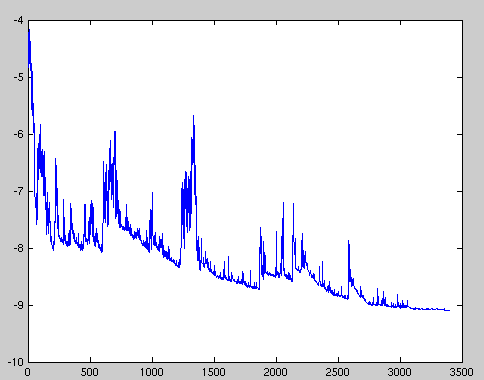
\includegraphics[height=7cm]{\pathroot/math/calculus/images/sgd_fluctuation.png}
    \caption{SGD波动}
    \label{fig:sgd_fluctuation}
\end{figure}

与批梯度下降法的收敛会使得损失函数陷入局部最小相比,
由于SGD的波动性,一方面,波动性使得SGD可以跳到新的和潜在更好的局部最优;
另一方面,这使得最终收敛到特定最小值的过程变得复杂,因为SGD会一直持续波动。
然而,已经证明当我们缓慢减小学习率,SGD与批梯度下降法具有相同的收敛行为,
对于非凸优化和凸优化,可以分别收敛到局部最小值和全局最小值。
与批梯度下降的代码相比,SGD的代码片段仅仅是在对训练样本的遍历和利用每一条样本计算梯度的过程中增加一层循环。
注意在每一次循环中,最好先随机打乱训练样本。


\subsubsection{Mini-batch gradient descent}
小批量梯度下降法最终结合了上述两种方法的优点,在每次更新时使用$n$个小批量训练样本:
\[
    \theta = \theta - \eta \cdot \nabla_{\theta}{J(\theta;x^{(i:i+n)};y^{(i:i+n)})}
\]

假设训练集有$m$个样本,每个mini-batch(训练集的一个子集)有$b$个样本,
那么,整个训练集可以分成$\frac{m}{b}$个mini-batch。

这种方法,
a) 减少参数更新的方差,这样可以得到更加稳定的收敛结果;
b) 可以利用最新的深度学习库中高度优化的矩阵优化方法,高效地求解每个小批量数据的梯度。

通常,小批量数据的大小在50到256之间,也可以根据不同的应用有所变化。
当训练神经网络模型时,小批量梯度下降法是典型的选择算法,当使用小批量梯度下降法时,也将其称为SGD。


\subsection{相关优化}
虽然Vanilla小批量梯度下降法并不能保证较好的收敛性,但是需要强调的是,这也给我们留下了如下的一些挑战:
\begin{itemize}
    \item 选择一个合适的学习率可能是困难的。
          学习率太小会导致收敛的速度很慢,学习率太大会妨碍收敛,导致损失函数在最小值附近波动甚至偏离最小值。

    \item 学习率调整试图在训练的过程中通过例如退火的方法调整学习率,
          即根据预定义的策略或者当相邻两代之间的下降值小于某个阈值时减小学习率。
          然而,策略和阈值需要预先设定好,因此无法适应数据集的特点。

    \item 此外,对所有的参数更新使用同样的学习率。
          如果数据是稀疏的,同时,特征的频率差异很大时,我们也许不想以同样的学习率更新所有的参数,
          对于出现次数较少的特征,我们对其执行更大的学习率。

    \item 高度非凸误差函数普遍出现在神经网络中,在优化这类函数时,
          另一个关键的挑战是使函数避免陷入无数次优的局部最小值。
          Dauphin等人指出出现这种困难实际上并不是来自局部最小值,
          而是来自鞍点,即那些在一个维度上是递增的,而在另一个维度上是递减的。
          这些鞍点通常被具有相同误差的点包围,因为在任意维度上的梯度都近似为0,所以SGD很难从这些鞍点中逃开。
\end{itemize}

\subsubsection{Momentum}

\[
    \Delta x_{t} = \rho \Delta x_{t-1} - \eta g_{t}
\]

SGD很难通过陡谷,即在一个维度上的表面弯曲程度远大于其他维度的区域,这种情况通常出现在局部最优点附近。
在这种情况下,SGD摇摆地通过陡谷的斜坡,同时,沿着底部到局部最优点的路径上只是缓慢地前进,
这个过程如图 \ref{fig:without_momentum} 所示。

\begin{figure}[H]
    \subfigure[普通SGD]{
        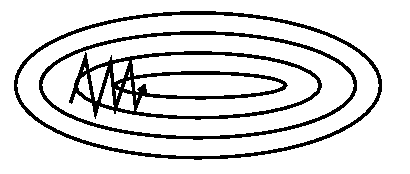
\includegraphics[scale=0.5]{\pathroot/math/calculus/images/without_momentum.png}
        \label{fig:without_momentum}
    }
    \subfigure[带有冲量的SGD]{
        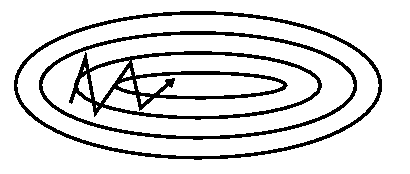
\includegraphics[scale=0.5]{\pathroot/math/calculus/images/with_momentum.png}
        \label{fig:with_momentum}
    }
    \caption{效果对比图}
\end{figure}

如图 \ref{fig:with_momentum} 所示,动量法是一种帮助SGD在相关方向上加速并抑制摇摆的一种方法。
动量法将历史步长的更新向量的一个分量 $\gamma$ 增加到当前的更新向量中
\begin{align*}
    & v_t = \gamma v_{t-1} + \eta \nabla_{\theta}{J(\theta)} \\
    & \theta = \theta - v_{t}
\end{align*}
动量项 $\gamma$ 通常设置为0.9或者类似的值。

从本质上说,动量法,就像我们从山上推下一个球,球在滚下来的过程中累积动量,变得越来越快
(直到达到终极速度,如果有空气阻力的存在,则 $\gamma < 1$)。
同样的事情也发生在参数的更新过程中:对于在梯度点处具有相同的方向的维度,其动量项增大,
对于在梯度点处改变方向的维度,其动量项减小。
因此,我们可以得到更快的收敛速度,同时可以减少摇摆。


相关实验:\url{https://github.com/hsmyy/zhihuzhuanlan/blob/master/momentum.ipynb}


\subsubsection{Nesterov accelerated gradient}

\url{https://github.com/WarBean/zhihuzhuanlan/blob/master/Momentum_Nesterov.ipynb}

\begin{align*}
    & v_t = \gamma v_{t-1} + \eta \nabla_{\theta}{J(\theta - \gamma v_{t-1})} \\
    & \theta = \theta - v_{t}
\end{align*}




\subsubsection{Adagrad}

\[
    \Delta x_{t} = -\frac{\eta}{\sqrt{\sum_{\tau = 1}^{t}{g_{\tau}^2}}} g_{t}
\]



\subsubsection{RMSprop}

\begin{align*}
    E[g^2]_{t} = 0.9 E[g^2]_{t-1} + 0.1 g_{t}^2 \\
    \theta_{t+1} = \theta_{t} - \frac{\eta}{\sqrt{E[g^2]_{t} + \epsilon}} g_{t}
\end{align*}



\subsubsection{Adadelta}
在梯度下降法中,学习率是一个需要人为设定的超参数,通常通过人工不断的调整,从而选择效果最好的学习率。
超过这个数值,模型训练的时候无法收敛;小于这个数值,又会导致模型收敛的很慢。
在很多问题中,选择合适的学习率需要靠直觉去选择,没有科学的选择方法。

Adadelta\cite{Zeiler:2012aa} 通过在每个维度上分别引入一个动态的学习率来避免人工选择学习率时遇到的问题。

\[
    E[g^2]_t = \rho E[g^2]_{t-1} + (1 - \rho)g_{t}^2
\]

据说,Adadelta 在深层 RNN 的架构中表现的很好(需要验证)。



\subsubsection{Adam}
\subsubsection{AdaMax}
\subsubsection{Nadam}
\subsubsection{Visualization of algorithms}
\subsubsection{Which optimizer to choose?}

\subsection{Parallelizing and distributing SGD}
\subsubsection{Hogwild!}
\subsubsection{Downpour SGD}
\subsubsection{Delay-tolerant Algorithms for SGD}
\subsubsection{TensorFlow}

\subsubsection{Elastic Averaging SGD}
\subsection{Additional strategies for optimizing SGD}
\subsubsection{Shuffling and Curriculum Learning}
\subsubsection{Batch normalization}

\subsubsection{Early Stopping}
\subsubsection{Gradient noise}


\subsubsection{Online}
随着互联网行业的蓬勃发展,数据变得越来越``廉价''。很多应用有实时的,不间断的训练数据产生。在线学习(Online Learning)算法就是充分利用实时数据的一个训练算法。

Online GD与mini-batch GD/SGD的区别在于,所有训练数据只用一次,然后丢弃。这样做的好处是可以获得模型的变化趋势。比如搜索广告的点击率(CTR)预估模型,网民的点击行为会随着时间改变。用batch算法(每天更新一次)一方面耗时较长(需要对所有历史数据重新训练);另一方面,无法及时反馈用户的点击行为迁移。而Online Leaning的算法可以实时的最终网民的点击行为迁移。

\subsection{深入阅读材料}
\begin{enumerate}
    \item \href{https://arxiv.org/abs/1606.04474}{Learning to learn by gradient descent by gradient descent}



\end{enumerate}






\section{牛顿迭代法}
\subsection{基本原理}
假设 $f(x) = 0$ 为待求解方程,利用传统方法求解,牛顿法求解方程的公式:
\[
f(x_0 + \Delta x) = f(x_0) + f'(x_0)\Delta x
\]
即
\[
    f(x) = f(x_0) + f'(x_0)(x - x_0)
\]

令 $f(x) = 0$,我们能够得到迭代公式:
\[
    x = x_0 - \frac{f(x_0)}{f'(x_0)} \Rightarrow x_{n+1} = x_n - \frac{f(x_n)}{f'(x_n)}
\]
通过逐次迭代,牛顿法将逐步逼近最优值,也就是方程的解。

解决 $f(x) = 0$ 的问题,我们用了一阶泰勒展开:
\[
    f(x) = f(x_0) + f'(x_0)*(x-x_0) + o((x-x_0))
\]
去掉末位高阶展开项,代入 $x = x_0 + \Delta x$,得到:
\[
    f(x) = f(x_0 + \Delta x) = f(x_0) + f'(x_0)\Delta x
\]


那么,要解决 $f'(x) = 0$ 的问题,我们就需要二阶泰勒展开:
\[
    f(x) = f(x_0) + f'(x_0)*(x-x_0) + \frac{f''(x_0)}{2}*(x-x_0)^2 + o((x-x_0)^2)
\]
去掉末位高阶展开项,代入 $x = x_0+\Delta x$,得到:
\[
    f(x) = f(x_0+\Delta x) = f(x_0) + f'(x_0) \Delta x + \frac{f''(x_0) (\Delta x)^2}{2}
\]
求导计算: $f'(x) = f'(x_0+\Delta x) = 0$,得到:
\[
    [f(x_0) + f'(x_0)(x−x_0) + \frac{f''(x_0)(x−x_0)^2}{2}]′ = 0
\]
整理:
\begin{align*}
    & f'(x_0) + f''(x_0)(x−x_0) = 0 \\
    & x = x_0 − \frac{f'(x_0)}{f''(x_0)} \Rightarrow  x_{n+1} = x_n - \frac{f'(x_n)}{f''(x_n)}
\end{align*}

\subsection{拟牛顿条件}

\section{拟牛顿法(Quasi-Newton)}
\subsection{DFP 算法}
\subsection{BFGS算法}
\subsection{L-BFGS 算法}


\section{共轭梯度法(Conjugate Gradient)}
学习资料
\begin{enumerate}
\item《最优化理论与方法》 袁亚湘 孙文瑜
\item http://blog.csdn.net/nocml/article/details/8287466
\item Updating Quasi-Newton Matrices with Limited Storage , Jorge Nocedal
\item Nonlinear Programming, second edition, Dimitri P. Bertsekas
\item《广告数据上的大规模机器学习》  夏粉
\end{enumerate}

\ifx\mlbook\undefined
    \bibliography{\pathroot/reference/reference.bib}
\end{document}

\fi


\chapter{线性代数}

\chapter{概率论与数理统计}

\chapter{信息论}

\ifx\notes\undefined
    \bibliography{\notesroot/reference/reference.bib}
\end{document}

\fi


\part{机器学习}
\def\mlnotes{}
\ifx\notes\undefined
    \providecommand{\notesroot}{..}
    \providecommand{\mlroot}{.}

    \title{机器学习}
    \author{Donald Cheung\\jianzhang9102@gmail.com}
    \date{\today\footnote{文档编写开始于2017年06月16日}}

    \documentclass[a4paper,10pt]{ctexbook}
\usepackage{xeCJK}
\usepackage{fontspec}
\usepackage{minted}
\usepackage[CJKbookmarks,colorlinks,linkcolor=red]{hyperref}
\usepackage{geometry}
\usepackage{amsmath}
\usepackage[format=hang,font=small,textfont=it]{caption}
\usepackage{float}
\usepackage{subfigure}
\usepackage[nottoc]{tocbibind}
\usepackage{bm}
\usepackage[table, x11names, dvipsnames]{xcolor}
\usepackage{color}
\usepackage{array, booktabs, boldline}
\usepackage{cellspace}
\usepackage{longtable}

\setmainfont{Times New Roman}
\setsansfont{Helvetica}
\setmonofont{Courier New}
\setCJKmainfont[BoldFont={SimHei},ItalicFont={SimHei}]{SimSun}
\setCJKsansfont{SimSun}
\setCJKmonofont{SimSun}

\setcounter{secnumdepth}{4}
\setcounter{tocdepth}{4}

\geometry{left=3.0cm,right=3.0cm,top=2.5cm,bottom=2.5cm}
\bibliographystyle{plain}

%%%%%%%%%%%%%%%%%%%%%%%%%%%%%%%%% minted setting %%%%%%%%%%%%%%%%%%%%%%%%%%%%%%%%%%%
\usemintedstyle{monokai}
\definecolor{bg}{HTML}{282828} % from https://github.com/kevinsawicki/monokai
%\defaultfontfeatures{}
\newfontfamily\noligsmonofamily[NFSSFamily=noligsmonofamily]{Courier}
\setminted{fontfamily=noligsmonofamily}

\renewcommand{\theFancyVerbLine}{%
    \sffamily \textcolor{Dandelion}{\scriptsize \oldstylenums{\arabic{FancyVerbLine}}}}

\newenvironment{jcode}[3]
{%
    \VerbatimEnvironment
    \begin{listing}[h]%
    \caption{#2}%
    \label{#3}%
    \begin{minted}[xleftmargin=18pt,
                   mathescape,
                   linenos,
                   numbersep=5pt,
                   bgcolor=bg,
                   frame=lines,
                   framesep=2mm,
                   fontsize=\footnotesize]{#1}%
}
{%
    \end{minted}
    \vspace{-25pt}%
    \end{listing}%
}
\renewcommand{\listingscaption}{代码}%from minted
\renewcommand{\listoflistingscaption}{代码列表}% from minted


\newenvironment{myquote}{\begin{quote}\kaishu\zihao{-5}}{\end{quote}}
\newcommand\degree{^\circ}
\newtheorem{thm}{定理}


\begin{document}
\maketitle
\tableofcontents
\listoflistings

\else
    \providecommand{\mlroot}{\notesroot/machine_learning}
\fi

\ifx\mlnotes\undefined
    \providecommand{\notesroot}{../..}
    \providecommand{\funcroot}{.}

    \title{机器学习常用函数}
    \author{Donald Cheung\\jianzhang9102@gmail.com}
    \date{\today\footnote{文档编写开始于2018年4月29日}}

    \documentclass[a4paper,10pt]{ctexbook}
\usepackage{xeCJK}
\usepackage{fontspec}
\usepackage{minted}
\usepackage[CJKbookmarks,colorlinks,linkcolor=red]{hyperref}
\usepackage{geometry}
\usepackage{amsmath}
\usepackage[format=hang,font=small,textfont=it]{caption}
\usepackage{float}
\usepackage{subfigure}
\usepackage[nottoc]{tocbibind}
\usepackage{bm}
\usepackage[table, x11names, dvipsnames]{xcolor}
\usepackage{color}
\usepackage{array, booktabs, boldline}
\usepackage{cellspace}
\usepackage{longtable}

\setmainfont{Times New Roman}
\setsansfont{Helvetica}
\setmonofont{Courier New}
\setCJKmainfont[BoldFont={SimHei},ItalicFont={SimHei}]{SimSun}
\setCJKsansfont{SimSun}
\setCJKmonofont{SimSun}

\setcounter{secnumdepth}{4}
\setcounter{tocdepth}{4}

\geometry{left=3.0cm,right=3.0cm,top=2.5cm,bottom=2.5cm}
\bibliographystyle{plain}

%%%%%%%%%%%%%%%%%%%%%%%%%%%%%%%%% minted setting %%%%%%%%%%%%%%%%%%%%%%%%%%%%%%%%%%%
\usemintedstyle{monokai}
\definecolor{bg}{HTML}{282828} % from https://github.com/kevinsawicki/monokai
%\defaultfontfeatures{}
\newfontfamily\noligsmonofamily[NFSSFamily=noligsmonofamily]{Courier}
\setminted{fontfamily=noligsmonofamily}

\renewcommand{\theFancyVerbLine}{%
    \sffamily \textcolor{Dandelion}{\scriptsize \oldstylenums{\arabic{FancyVerbLine}}}}

\newenvironment{jcode}[3]
{%
    \VerbatimEnvironment
    \begin{listing}[h]%
    \caption{#2}%
    \label{#3}%
    \begin{minted}[xleftmargin=18pt,
                   mathescape,
                   linenos,
                   numbersep=5pt,
                   bgcolor=bg,
                   frame=lines,
                   framesep=2mm,
                   fontsize=\footnotesize]{#1}%
}
{%
    \end{minted}
    \vspace{-25pt}%
    \end{listing}%
}
\renewcommand{\listingscaption}{代码}%from minted
\renewcommand{\listoflistingscaption}{代码列表}% from minted


\newenvironment{myquote}{\begin{quote}\kaishu\zihao{-5}}{\end{quote}}
\newcommand\degree{^\circ}
\newtheorem{thm}{定理}


\begin{document}
\maketitle
\tableofcontents
\listoflistings

\else
    \providecommand{\funcroot}{\mlroot/function}
\fi

\chapter{机器学习常用函数}

\section{模型评估}

\subsection{Accuracy}
Accuracy is the count of predictions where your predicted value equals the actual value.
Accuracy is not always a good indicator because of its yes or no nature.

\subsection{log loss}

\begin{jcode}{python}{log loss计算}{code:logloss}
import numpy as np
def log_loss(true_y, pred_h):
    return -np.mean(true_y * np.log(pred_h) + (1 - true_y) * np.log(1 - pred_h))
\end{jcode}

\subsection{ROC与AUC}

\ifx\mlnotes\undefined
    \bibliography{\notesroot/reference/reference.bib}
\end{document}

\fi


\ifx\mlnotes\undefined
    \providecommand{\notesroot}{../..}

    \title{Recurrent Neural Network}
    \author{Donald Cheung\\jianzhang9102@gmail.com}
    \date{\today\footnote{文档编写开始于2018年4月29日}}

    \documentclass[a4paper,10pt]{ctexbook}
\usepackage{xeCJK}
\usepackage{fontspec}
\usepackage{minted}
\usepackage[CJKbookmarks,colorlinks,linkcolor=red]{hyperref}
\usepackage{geometry}
\usepackage{amsmath}
\usepackage[format=hang,font=small,textfont=it]{caption}
\usepackage{float}
\usepackage{subfigure}
\usepackage[nottoc]{tocbibind}
\usepackage{bm}
\usepackage[table, x11names, dvipsnames]{xcolor}
\usepackage{color}
\usepackage{array, booktabs, boldline}
\usepackage{cellspace}
\usepackage{longtable}

\setmainfont{Times New Roman}
\setsansfont{Helvetica}
\setmonofont{Courier New}
\setCJKmainfont[BoldFont={SimHei},ItalicFont={SimHei}]{SimSun}
\setCJKsansfont{SimSun}
\setCJKmonofont{SimSun}

\setcounter{secnumdepth}{4}
\setcounter{tocdepth}{4}

\geometry{left=3.0cm,right=3.0cm,top=2.5cm,bottom=2.5cm}
\bibliographystyle{plain}

%%%%%%%%%%%%%%%%%%%%%%%%%%%%%%%%% minted setting %%%%%%%%%%%%%%%%%%%%%%%%%%%%%%%%%%%
\usemintedstyle{monokai}
\definecolor{bg}{HTML}{282828} % from https://github.com/kevinsawicki/monokai
%\defaultfontfeatures{}
\newfontfamily\noligsmonofamily[NFSSFamily=noligsmonofamily]{Courier}
\setminted{fontfamily=noligsmonofamily}

\renewcommand{\theFancyVerbLine}{%
    \sffamily \textcolor{Dandelion}{\scriptsize \oldstylenums{\arabic{FancyVerbLine}}}}

\newenvironment{jcode}[3]
{%
    \VerbatimEnvironment
    \begin{listing}[h]%
    \caption{#2}%
    \label{#3}%
    \begin{minted}[xleftmargin=18pt,
                   mathescape,
                   linenos,
                   numbersep=5pt,
                   bgcolor=bg,
                   frame=lines,
                   framesep=2mm,
                   fontsize=\footnotesize]{#1}%
}
{%
    \end{minted}
    \vspace{-25pt}%
    \end{listing}%
}
\renewcommand{\listingscaption}{代码}%from minted
\renewcommand{\listoflistingscaption}{代码列表}% from minted


\newenvironment{myquote}{\begin{quote}\kaishu\zihao{-5}}{\end{quote}}
\newcommand\degree{^\circ}
\newtheorem{thm}{定理}


\begin{document}
\maketitle
\tableofcontents
\listoflistings

\fi

\chapter{Recurrent Neural Network}

\section{BPTT}
\[
    \frac{\partial E_3}{\partial W}=\sum_{k=0}^{3}{
        \frac{\partial E_3}{\partial \hat{y}_3}
        \frac{\partial \hat{y}_3}{\partial s_3}
        \frac{\partial s_3}{\partial s_k}
        \frac{\partial s_k}{\partial W}
    }
\]

\[
    \frac{\partial E_t}{\partial W}=\sum_{k=0}^{t}{
        \frac{\partial E_t}{\partial \hat{y}_t}
        \frac{\partial \hat{y}_t}{\partial s_t}
        \frac{\partial s_t}{\partial s_k}
        \frac{\partial s_k}{\partial W}
    }
\]

\[
    \frac{\partial s_t}{\partial s_k}=\prod_{j=k+1}^{t} \frac{\partial s_j}{\partial s_{j-1}}
\]

\section{LSTM}



\section{相关应用}

\subsection{RNN文本生成}
\begin{itemize}
    \item \href{https://karpathy.github.io/2015/05/21/rnn-effectiveness/}{The Unreasonable Effectiveness of Recurrent Neural Networks}
        \subitem \url{https://github.com/karpathy/char-rnn}
        \subitem \url{https://github.com/karpathy/neuraltalk}
    \item \href{https://arxiv.org/abs/1412.7755}{MULTIPLE OBJECT RECOGNITION WITH VISUAL ATTENTION}
    \item \href{https://arxiv.org/abs/1502.04623}{DRAW: A Recurrent Neural Network For Image Generation}
    \item \href{http://www.cs.utoronto.ca/~ilya/pubs/2011/LANG-RNN.pdf}{Generating Text with Recurrent Neural Networks}
\item \href{https://arxiv.org/abs/1308.0850}{Generating Sequences With Recurrent Neural Networks}
\end{itemize}


\section{待整理}

\href{https://arxiv.org/pdf/1406.1078v3.pdf}{Learning Phrase Representations using RNN Encoder-Decoder for Statistical Machine Translation}

\href{http://www.cs.utoronto.ca/~ilya/pubs/ilya_sutskever_phd_thesis.pdf}{Ilya Sutskever, Training Recurrent Neural Networks, Thesis, 2013}

\href{https://arxiv.org/abs/1503.04069}{LSTM: A Search Space Odyssey}

\href{https://arxiv.org/abs/1506.00019}{A Critical Review of Recurrent Neural Networks for Sequence Learning}

\href{https://jramapuram.github.io/ramblings/rnn-backrpop/}{BLOG: RNN Backprop Through Time Equations}

vanilla RNNs trained with BPTT \href{http://www.jmlr.org/proceedings/papers/v28/pascanu13.pdf}{have difficulties} learning long-term dependencies (e.g. dependencies between steps that are far apart) due to what is called the vanishing/exploding gradient problem. There exists some machinery to deal with these problems, and certain types of RNNs (like LSTMs) were specifically designed to get around them.

\[
\begin{aligned}
C_{i,j} & = -\tilde{P_{ij}} * o_{i,j} + log(1 + e^{o_{i,j}})\\o_{i,j} & = o_i - o_j\\\tilde{P_{i,j}} & = \{0, 0.5, 1\} \ or \ \{0, 1\}
\end{aligned}
\]

Cosine Similarity Layer. The cosine similarity equation is here.
\[similarity = cos(\theta) = {\mathbf{a} \cdot \mathbf{b} \over \|\mathbf{a}\| \|\mathbf{b}\|}\]
The size of a is M, size of b is M*N, Similarity will be calculated N times by step M. The output size is N. The scale will be multiplied to similarity.

Note that the above computation is for one sample. Multiple samples are processed in one batch.

\begin{table}[H]
\centering
\begin{tabular}{|l|l|l|}
\hline
Neural Layer & Description & Index variable\\
\hline
$x(t)$ & input layer & $i$ \\
$s(t-1)$ & previous hidden (state) layer & $h$ \\
$s(t)$ & hidden (state) layer & $j$ \\
$y(t)$ & output layer & $k$ \\
\hline
\end{tabular}%
\caption{Notations in the recurrent neural network.}
\label{tab:rnn-notations}
\end{table}

%\inputminted{python}{\pathroot/reference/code/bptt.py}

\begin{itemize}
\item Hochreiter S, Schmidhuber J. \href{http://web.eecs.utk.edu/~itamar/courses/ECE-692/Bobby_paper1.pdf}{Long short-term memory[J]}. Neural computation, 1997, 9(8): 1735-1780.
\item Bengio Y, Simard P, Frasconi P. \href{http://www-dsi.ing.unifi.it/~paolo/ps/tnn-94-gradient.pdf}{Learning long-term dependencies with gradient descent is difficult[J]}. IEEE transactions on neural networks, 1994, 5(2): 157-166.
\item \href{https://arxiv.org/pdf/1610.09038.pdf}{Professor Forcing: A New Algorithm for Training Recurrent Networks}
\item \href{http://ir.hit.edu.cn/~jguo/docs/notes/bptt.pdf}{BackPropagation Through Time}
\item \href{http://nn.cs.utexas.edu/downloads/papers/james.sardnet.pdf}{SARDNET: A Self-Organizing Feature Map for Sequences*}
\item \href{http://colah.github.io/posts/2015-08-Understanding-LSTMs/}{Understanding LSTMs}
\end{itemize}

\begin{itemize}
\item $x_t$是时刻$t$的输入。例如,$x_1$可以是一个one-hot的稀疏向量,表示一个句子中的第二个单词。
\item $s_t$是时刻$t$的隐层状态,是网络的记忆单元。$s_t$的计算依赖于当前时刻的输入以及之前的隐层状态值:$s_t=f(Ux_t+Ws_{t-1})$。函数$f$通常是非线性函数,例如$tanh$或者是$ReLU$。
\item $o_t$是时刻$t$的输出。例如,当我们需要预测一个句子中的下一个词时,$o_t$为词典中每个词的概率,也即$o_t=softmax(Vs_t)$
\item 需要注意的是,RNN中的$U,V,W$参数是共享的。
\end{itemize}

\subsection{A Critical Review of Recurrent Neural Networks for Sequence Learning}

\subsection{Neural Turing Machines}
\href{Neural Turing Machines}{https://arxiv.org/abs/1410.5401}

\subsection{Attention}
\href{https://distill.pub/2016/augmented-rnns/}{Attention and Augmented Recurrent Neural Networks}

\href{https://arxiv.org/abs/1706.03762}{Attention Is All You Need}

\subsubsection{Soft Attention}
The concept of attention is the most interesting recent architectural innovation in neural networks.

\subsubsection{Hard Attention}
\href{Inferring Algorithmic Patterns with Stack-Augmented Recurrent Nets}{https://arxiv.org/abs/1503.01007}
\href{Reinforcement Learning Neural Turing Machines - Revised}{https://arxiv.org/abs/1505.00521}
\href{Show, Attend and Tell: Neural Image Caption Generation with Visual Attention}{https://arxiv.org/abs/1502.03044}


\textbf{RNN实现}

\href{http://www.wildml.com/2015/09/recurrent-neural-networks-tutorial-part-1-introduction-to-rnns/}{Recurrent Neural Networks Tutorial, Part 1 – Introduction to RNNs}

\subsubsection{Initialization}
We start by declaring a RNN class an initializing our parameters. I'm calling this class RNNNumpy because we will implement a Theano version later. Initializing the parameters $U$,$V$ and $W$ is a bit tricky. We can't just initialize them to 0's because that would result in symmetric calculations in all our layers. We must initialize them randomly. Because proper initialization seems to have an impact on training results there has been lot of research in this area. It turns out that the best initialization depends on the activation function ($\tanh$ in our case) and one recommended approach is to initialize the weights randomly in the interval from $\left[-\frac{1}{\sqrt{n}}, \frac{1}{\sqrt{n}}\right]$ where n is the number of incoming connections from the previous layer. This may sound overly complicated, but don't worry too much it. As long as you initialize your parameters to small random values it typically works out fine.

\begin{minted}[breaklines,tabsize=2,linenos]{python}
class RNNNumpy(object):
    def __init__(self, word_dim, hidden_dim=100, bptt_truncate=4):
        # Assign instance variables
        self.word_dim = word_dim
        self.hidden_dim = hidden_dim
        self.bptt_truncate = bptt_truncate
        # Randomly initialize the network parameters
        self.U = np.random.uniform(-np.sqrt(1./word_dim), np.sqrt(1./word_dim),
                                    (hidden_dim, word_dim))
        self.V = np.random.uniform(-np.sqrt(1./hidden_dim),np.sqrt(1./hidden_dim),
                                    (word_dim, hidden_dim))
        self.W = np.random.uniform(-np.sqrt(1./hidden_dim), np.sqrt(1./hidden_dim),
                                    (hidden_dim, hidden_dim))
\end{minted}
Above, word\_dim is the size of our vocabulary, and hidden\_dim is the size of our hidden layer (we can pick it). Don't worry about the bptt\_truncate parameter for now, we'll explain what that is later.

\subsubsection{Forward Propagation}
Next, let's implement the forward propagation (predicting word probabilities) defined by our equations above:

\begin{minted}[breaklines,tabsize=2,linenos]{python}
def forward_propagation(self, x):
    # The total number of time steps
    T = len(x)
    # During forward propagation we save all hidden states in s because need them later.
    # We add one additional element for the initial hidden, which we set to 0
    s = np.zeros((T + 1, self.hidden_dim))
    s[-1] = np.zeros(self.hidden_dim)
    # The outputs at each time step. Again, we save them for later.
    o = np.zeros((T, self.word_dim))
    # For each time step...
    for t in np.arange(T):
        # Note that we are indxing U by x[t].
        #This is the same as multiplying U with a one-hot vector.
        s[t] = np.tanh(self.U[:,x[t]] + self.W.dot(s[t-1]))
        o[t] = softmax(self.V.dot(s[t]))
    return [o, s]
 
RNNNumpy.forward_propagation = forward_propagation
\end{minted}

We not only return the calculated outputs, but also the hidden states. We will use them later to calculate the gradients, and by returning them here we avoid duplicate computation. Each o\_t is a vector of probabilities representing the words in our vocabulary, but sometimes, for example when evaluating our model, all we want is the next word with the highest probability. We call this function predict:

\begin{minted}[breaklines,tabsize=2,linenos]{python}
def predict(self, x):
    # Perform forward propagation and return index of the highest score
    o, s = self.forward_propagation(x)
    return np.argmax(o, axis=1)

    RNNNumpy.predict = predict
\end{minted}


\subsubsection{Calculating the Loss}
To train our network we need a way to measure the errors it makes. We call this the loss function $L$, and our goal is find the parameters $U$,$V$ and $W$ that minimize the loss function for our training data. A common choice for the loss function is the cross-entropy loss. If we have $N$ training examples (words in our text) and C classes (the size of our vocabulary) then the loss with respect to our predictions o and the true labels y is given by:

\[
\begin{aligned}
    L(y,o) = - \frac{1}{N} \sum_{n \in N} y_{n} \log o_{n}
\end{aligned}  
\]

The formula looks a bit complicated, but all it really does is sum over our training examples and add to the loss based on how off our prediction are. The further away $y$ (the correct words) and $o$ (our predictions), the greater the loss will be. We implement the function calculate\_loss:

\begin{minted}[breaklines,tabsize=2,linenos]{python}
def calculate_total_loss(self, x, y):
    L = 0
    # For each sentence...
    for i in np.arange(len(y)):
        o, s = self.forward_propagation(x[i])
        # We only care about our prediction of the "correct" words
        correct_word_predictions = o[np.arange(len(y[i])), y[i]]
        # Add to the loss based on how off we were
        L += -1 * np.sum(np.log(correct_word_predictions))
    return L
 
def calculate_loss(self, x, y):
    # Divide the total loss by the number of training examples
    N = np.sum((len(y_i) for y_i in y))
    return self.calculate_total_loss(x,y)/N
 
RNNNumpy.calculate_total_loss = calculate_total_loss
RNNNumpy.calculate_loss = calculate_loss
\end{minted}

Let's take a step back and think about what the loss should be for random predictions. That will give us a baseline and make sure our implementation is correct. We have $C$ words in our vocabulary, so each word should be (on average) predicted with probability $\frac{1}{C}$, which would yield a loss of $L = -\frac{1}{N} N \log\frac{1}{C} = \log C$:

\begin{minted}[breaklines,tabsize=2,linenos]{python}
# Limit to 1000 examples to save time
print "Expected Loss for random predictions: %f" % np.log(vocabulary_size)
print "Actual loss: %f" % model.calculate_loss(X_train[:1000], y_train[:1000])

Expected Loss for random predictions: 8.987197
Actual loss: 8.987440
\end{minted}

Pretty close! Keep in mind that evaluating the loss on the full dataset is an expensive operation and can take hours if you have a lot of data!

\subsubsection{Training the RNN with SGD and Backpropagation Through Time (BPTT)}
Remember that we want to find the parameters $U$,$V$ and $W$ that minimize the total loss on the training data. The most common way to do this is SGD, Stochastic Gradient Descent. The idea behind SGD is pretty simple. We iterate over all our training examples and during each iteration we nudge the parameters into a direction that reduces the error. These directions are given by the gradients on the loss: $\frac{\partial L}{\partial U}$, $\frac{\partial L}{\partial V}$, $\frac{\partial L}{\partial W}$. SGD also needs a learning rate, which defines how big of a step we want to make in each iteration. SGD is the most popular optimization method not only for Neural Networks, but also for many other Machine Learning algorithms. As such there has been a lot of research on how to optimize SGD using batching, parallelism and adaptive learning rates. Even though the basic idea is simple, implementing SGD in a really efficient way can become very complex. If you want to learn more about SGD \href{http://cs231n.github.io/optimization-1/}{this} is a good place to start. Due to its popularity there are a wealth of tutorials floating around the web, and I don't want to duplicate them here. I'll implement a simple version of SGD that should be understandable even without a background in optimization.

But how do we calculate those gradients we mentioned above? In a \href{http://www.wildml.com/2015/09/implementing-a-neural-network-from-scratch/}{traditional Neural Network} we do this through the backpropagation algorithm. In RNNs we use a slightly modified version of the this algorithm called \emph{Backpropagation Through Time (BPTT)}. Because the parameters are shared by all time steps in the network, the gradient at each output depends not only on the calculations of the current time step, but also the previous time steps. If you know calculus, it really is just applying the chain rule. The next part of the tutorial will be all about BPTT, so I won't go into detailed derivation here. For a general introduction to backpropagation check out \href{http://colah.github.io/posts/2015-08-Backprop/}{this} and this \href{http://cs231n.github.io/optimization-2/}{post}. For now you can treat \textbf{BPTT} as a black box. It takes as input a training example $(x,y)$ and returns the gradients $\frac{\partial L}{\partial U}$, $\frac{\partial L}{\partial V}$, $\frac{\partial L}{\partial W}$.

\begin{minted}[breaklines,tabsize=2,linenos]{python}
def bptt(self, x, y):
    T = len(y)
    # Perform forward propagation
    o, s = self.forward_propagation(x)
    # We accumulate the gradients in these variables
    dLdU = np.zeros(self.U.shape)
    dLdV = np.zeros(self.V.shape)
    dLdW = np.zeros(self.W.shape)
    delta_o = o
    delta_o[np.arange(len(y)), y] -= 1.
    # For each output backwards...
    for t in np.arange(T)[::-1]:
        dLdV += np.outer(delta_o[t], s[t].T)
        # Initial delta calculation
        delta_t = self.V.T.dot(delta_o[t]) * (1 - (s[t] ** 2))
        # Backpropagation through time (for at most self.bptt_truncate steps)
        for bptt_step in np.arange(max(0, t-self.bptt_truncate), t+1)[::-1]:
            # print "Backpropagation step t=%d bptt step=%d " % (t, bptt_step)
            dLdW += np.outer(delta_t, s[bptt_step-1])              
            dLdU[:,x[bptt_step]] += delta_t
            # Update delta for next step
            delta_t = self.W.T.dot(delta_t) * (1 - s[bptt_step-1] ** 2)
    return [dLdU, dLdV, dLdW]
 
RNNNumpy.bptt = bptt
\end{minted}

\subsubsection{Gradient Checking}
Whenever you implement backpropagation it is good idea to also implement gradient checking, which is a way of verifying that your implementation is correct. The idea behind gradient checking is that derivative of a parameter is equal to the slope at the point, which we can approximate by slightly changing the parameter and then dividing by the change:

\[
\begin{aligned}
\frac{\partial L}{\partial \theta} \approx \lim_{h \to 0}\frac{J(\theta + h) - J(\theta - h)}{2h}
\end{aligned}
\]

We then compare the gradient we calculated using backpropagation to the gradient we estimated with the method above. If there's no large difference we are good. The approximation needs to calculate the total loss for every parameter, so that gradient checking is very expensive (remember, we had more than a million parameters in the example above). So it's a good idea to perform it on a model with a smaller vocabulary.

\begin{minted}[breaklines,tabsize=2,linenos]{python}
def gradient_check(self, x, y, h=0.001, error_threshold=0.01):
    # Calculate the gradients using backpropagation. We want to checker if these are correct.
    bptt_gradients = self.bptt(x, y)
    # List of all parameters we want to check.
    model_parameters = ['U', 'V', 'W']
    # Gradient check for each parameter
    for pidx, pname in enumerate(model_parameters):
        # Get the actual parameter value from the mode, e.g. model.W
        parameter = operator.attrgetter(pname)(self)
        print "Performing gradient check for parameter %s with size %d." % (pname, np.prod(parameter.shape))
        # Iterate over each element of the parameter matrix, e.g. (0,0), (0,1), ...
        it = np.nditer(parameter, flags=['multi_index'], op_flags=['readwrite'])
        while not it.finished:
            ix = it.multi_index
            # Save the original value so we can reset it later
            original_value = parameter[ix]
            # Estimate the gradient using (f(x+h) - f(x-h))/(2*h)
            parameter[ix] = original_value + h
            gradplus = self.calculate_total_loss([x],[y])
            parameter[ix] = original_value - h
            gradminus = self.calculate_total_loss([x],[y])
            estimated_gradient = (gradplus - gradminus)/(2*h)
            # Reset parameter to original value
            parameter[ix] = original_value
            # The gradient for this parameter calculated using backpropagation
            backprop_gradient = bptt_gradients[pidx][ix]
            # calculate The relative error: (|x - y|/(|x| + |y|))
            relative_error = np.abs(backprop_gradient - estimated_gradient)/(np.abs(backprop_gradient) + np.abs(estimated_gradient))
            # If the error is to large fail the gradient check
            if relative_error &gt; error_threshold:
                print "Gradient Check ERROR: parameter=%s ix=%s" % (pname, ix)
                print "+h Loss: %f" % gradplus
                print "-h Loss: %f" % gradminus
                print "Estimated_gradient: %f" % estimated_gradient
                print "Backpropagation gradient: %f" % backprop_gradient
                print "Relative Error: %f" % relative_error
                return
            it.iternext()
        print "Gradient check for parameter %s passed." % (pname)
 
RNNNumpy.gradient_check = gradient_check
 
# To avoid performing millions of expensive calculations we use a smaller vocabulary size for checking.
grad_check_vocab_size = 100
np.random.seed(10)
model = RNNNumpy(grad_check_vocab_size, 10, bptt_truncate=1000)
model.gradient_check([0,1,2,3], [1,2,3,4])
\end{minted}


\subsubsection{SGD Implementation}
Now that we are able to calculate the gradients for our parameters we can implement SGD. I like to do this in two steps: 1. A function sdg\_step that calculates the gradients and performs the updates for one batch. 2. An outer loop that iterates through the training set and adjusts the learning rate.

\begin{minted}[breaklines,tabsize=2,linenos]{python}
# Performs one step of SGD.
def numpy_sdg_step(self, x, y, learning_rate):
    # Calculate the gradients
    dLdU, dLdV, dLdW = self.bptt(x, y)
    # Change parameters according to gradients and learning rate
    self.U -= learning_rate * dLdU
    self.V -= learning_rate * dLdV
    self.W -= learning_rate * dLdW
 
RNNNumpy.sgd_step = numpy_sdg_step
\end{minted}

\begin{minted}[breaklines,tabsize=2,linenos]{python}
# Outer SGD Loop
# - model: The RNN model instance
# - X_train: The training data set
# - y_train: The training data labels
# - learning_rate: Initial learning rate for SGD
# - nepoch: Number of times to iterate through the complete dataset
# - evaluate_loss_after: Evaluate the loss after this many epochs
def train_with_sgd(model, X_train, y_train, learning_rate=0.005, nepoch=100, evaluate_loss_after=5):
    # We keep track of the losses so we can plot them later
    losses = []
    num_examples_seen = 0
    for epoch in range(nepoch):
        # Optionally evaluate the loss
        if (epoch % evaluate_loss_after == 0):
            loss = model.calculate_loss(X_train, y_train)
            losses.append((num_examples_seen, loss))
            time = datetime.now().strftime('%Y-%m-%d %H:%M:%S')
            print "%s: Loss after num_examples_seen=%d epoch=%d: %f" % (time, num_examples_seen, epoch, loss)
            # Adjust the learning rate if loss increases
            if (len(losses) > 1 and losses[-1][1] > losses[-2][1]):
                learning_rate = learning_rate * 0.5 
                print "Setting learning rate to %f" % learning_rate
            sys.stdout.flush()
        # For each training example...
        for i in range(len(y_train)):
            # One SGD step
            model.sgd_step(X_train[i], y_train[i], learning_rate)
            num_examples_seen += 1
\end{minted}

Done! Let's try to get a sense of how long it would take to train our network:

\begin{minted}[breaklines,tabsize=2,linenos]{python}
np.random.seed(10)
model = RNNNumpy(vocabulary_size)
%timeit model.sgd_step(X_train[10], y_train[10], 0.005)
\end{minted}


Uh-oh, bad news. One step of SGD takes approximately 350 milliseconds on my laptop. We have about 80,000 examples in our training data, so one epoch (iteration over the whole data set) would take several hours. Multiple epochs would take days, or even weeks! And we’re still working with a small dataset compared to what’s being used by many of the companies and researchers out there. What now?

Fortunately there are many ways to speed up our code. We could stick with the same model and make our code run faster, or we could modify our model to be less computationally expensive, or both. Researchers have identified many ways to make models less computationally expensive, for example by using a hierarchical softmax or adding projection layers to avoid the large matrix multiplications (see also \href{http://arxiv.org/pdf/1301.3781.pdf}{here} or \href{http://www.fit.vutbr.cz/research/groups/speech/publi/2011/mikolov\_icassp2011\_5528.pdf}{here}). But I want to keep our model simple and go the first route: Make our implementation run faster using a GPU. Before doing that though, let’s just try to run SGD with a small dataset and check if the loss actually decreases:


\begin{minted}[breaklines,tabsize=2,linenos]{python}
np.random.seed(10)
# Train on a small subset of the data to see what happens
model = RNNNumpy(vocabulary_size)
losses = train_with_sgd(model, X_train[:100], y_train[:100], nepoch=10, evaluate_loss_after=1)

2015-09-30 10:08:19: Loss after num_examples_seen=0 epoch=0: 8.987425
2015-09-30 10:08:35: Loss after num_examples_seen=100 epoch=1: 8.976270
2015-09-30 10:08:50: Loss after num_examples_seen=200 epoch=2: 8.960212
2015-09-30 10:09:06: Loss after num_examples_seen=300 epoch=3: 8.930430
2015-09-30 10:09:22: Loss after num_examples_seen=400 epoch=4: 8.862264
2015-09-30 10:09:38: Loss after num_examples_seen=500 epoch=5: 6.913570
2015-09-30 10:09:53: Loss after num_examples_seen=600 epoch=6: 6.302493
2015-09-30 10:10:07: Loss after num_examples_seen=700 epoch=7: 6.014995
2015-09-30 10:10:24: Loss after num_examples_seen=800 epoch=8: 5.833877
2015-09-30 10:10:39: Loss after num_examples_seen=900 epoch=9: 5.710718
\end{minted}

Good, it seems like our implementation is at least doing something useful and decreasing the loss, just like we wanted.


\subsubsection{Generating Text}
Now that we have our model we can ask it to generate new text for us! Let’s implement a helper function to generate new sentences:

\begin{minted}[breaklines,tabsize=2,linenos]{python}
def generate_sentence(model):
    # We start the sentence with the start token
    new_sentence = [word_to_index[sentence_start_token]]
    # Repeat until we get an end token
    while not new_sentence[-1] == word_to_index[sentence_end_token]:
        next_word_probs = model.forward_propagation(new_sentence)
        sampled_word = word_to_index[unknown_token]
        # We don't want to sample unknown words
        while sampled_word == word_to_index[unknown_token]:
            samples = np.random.multinomial(1, next_word_probs[-1])
            sampled_word = np.argmax(samples)
        new_sentence.append(sampled_word)
    sentence_str = [index_to_word[x] for x in new_sentence[1:-1]]
    return sentence_str
 
num_sentences = 10
senten_min_length = 7
 
for i in range(num_sentences):
    sent = []
    # We want long sentences, not sentences with one or two words
    while len(sent) < senten_min_length:
        sent = generate_sentence(model)
    print " ".join(sent)
\end{minted}
Looking at the generated sentences there are a few interesting things to note. The model successfully learn syntax. It properly places commas (usually before and's and or's) and ends sentence with punctuation. Sometimes it mimics internet speech such as multiple exclamation marks or smileys.

However, the vast majority of generated sentences don't make sense or have grammatical errors (I really picked the best ones above). One reason could be that we did not train our network long enough (or didn't use enough training data). That may be true, but it's most likely not the main reason. Our vanilla RNN can't generate meaningful text because it's unable to learn dependencies between words that are several steps apart. That's also why RNNs failed to gain popularity when they were first invented. They were beautiful in theory but didn't work well in practice, and we didn't immediately understand why.

Fortunately, the difficulties in training RNNs are much \href{http://arxiv.org/abs/1211.5063}{better understood} now. In the next part of this tutorial we will explore the Backpropagation Through Time (BPTT) algorithm in more detail and demonstrate what's called the vanishing gradient problem. This will motivate our move to more sophisticated RNN models, such as LSTMs, which are the current state of the art for many tasks in NLP (and can generate much better reddit comments!). \textbf{Everything you learned in this tutorial also applies to LSTMs and other RNN models, so don't feel discouraged if the results for a vanilla RNN are worse then you expected}.


\subsection{Machine Translation}
Machine Translation is similar to language modeling in that our input is a sequence of words in our source language (e.g. German). We want to output a sequence of words in our target language (e.g. English). A key difference is that our output only starts after we have seen the complete input, because the first word of our translated sentences may require information captured from the complete input sequence.

%\begin{figure}[ht]
%    \centering
%    \includegraphics[scale=0.3]{\pathroot/reference/pictures/rnn_machine_translation.png}
%    \caption{RNN for machine Translation}
%    \label{fig:rnn_machine_translation}
%\end{figure}
%\ref{fig:rnn_machine_translation} RNN for Machine Translation. Image Source: \url{http://cs224d.stanford.edu/lectures/CS224d-Lecture8.pdf}


Research papers about Machine Translation:
\begin{itemize}
\item \href{http://www.aclweb.org/anthology/P14-1140.pdf}{A Recursive Recurrent Neural Network for Statistical Machine Translation}
\item \href{http://papers.nips.cc/paper/5346-sequence-to-sequence-learning-with-neural-networks.pdf}{Sequence to Sequence Learning with Neural Networks}
\item \href{http://research.microsoft.com/en-us/um/people/gzweig/Pubs/EMNLP2013RNNMT.pdf}{Joint Language and Translation Modeling with Recurrent Neural Networks}
\end{itemize}

\subsection{Speech Recognition}
Given an input sequence of acoustic signals from a sound wave, we can predict a sequence of phonetic segments together with their probabilities.

Research papers about Speech Recognition:
\begin{itemize}
\item \href{http://www.jmlr.org/proceedings/papers/v32/graves14.pdf}{Towards End-to-End Speech Recognition with Recurrent Neural Networks}
\end{itemize}


\subsection{Generating Image Descriptions}
Together with convolutional Neural Networks, RNNs have been used as part of a model to \href{http://cs.stanford.edu/people/karpathy/deepimagesent/}{generate descriptions} for unlabeled images. It's quite amazing how well this seems to work. The combined model even aligns the generated words with features found in the images.

%\begin{figure}[ht]
%    \centering
%    \includegraphics[scale=0.3]{\pathroot/reference/pictures/rnn_image_notation.png}
%    \caption{RNN for Generating Image Descriptions}
%    \label{fig:rnn_image_notation}
%\end{figure}
%\ref{fig:rnn_image_notation}
Deep Visual-Semantic Alignments for Generating Image Descriptions.
Source: \url{http://cs.stanford.edu/people/karpathy/deepimagesent/}


\subsubsection{百度内部--土星五号(新触发引擎)}
\textbf{这是百度内部2016年最高奖的三个项目之一}

``土星五号"这个名字取自人类历史上使用过的自重最大的运载火箭,高达110.6米,起飞重量3038吨,总推力达3400吨左右,曾将阿波罗成功送上月球。``土星五号"的负责人陈志杰告诉小编,这个名字寄托了他们9个人的心愿:希望``新触发引擎"能够像伟大的``土星五号"一样为百度变现提供强大的推力。

广告候选少,召回要求高,质量控制难。这是摆在``土星五号"这个小型团队的三个重大困难。整个凤巢检索端系统呈漏斗状分布,触发子系统位于漏斗最上部。从触发子系统到最终展现环节经过层层过滤,剩下广告结果不到初始环节的5\%,为了保证最终展现环节有足够广告结果,触发子系统的召回能力至关重要。但另一方面,客户提交到广告数仅有6亿左右,可谓``巧妇难为无米之炊",当广告索引充足时,简单的触发策略就能匹配到足量合适的广告,而广告索引少时则需要更强悍的触发算法。

传统触发系统都由检索和校验两部分组成,匹配算法是基于字面相似度的,召回不高。新触发引擎从判别式到生成式,引入AI机器学习技术全面重构触发系统,构建了高度智能化的触发引擎。在判别式触发中,通过采用DNN、knowledge distilling等技术做强相关性校验,从而能够支持多粒度灵活检索,召回量提升58.5\%。仅仅做到这一步,``土星五号"团队当然是不满足的。他们又创造性的提出了生成式触发模型,通过neural seq2seq generation方式做广告触发,这也是业界首次使用``生成式"方式做广告触发。 

针对业务需求与线上性能要求,``土星五号"做了一系列技术创新:定向解码、自归一化、路径优选、动态剪枝、弹性计算、分级计算、模型结构优化、硬件加速等等,最终将一个单次预测需要计算32亿浮点乘法、耗时2秒的大家伙,性能优化166倍,实现高并发实时计算,日处理33亿次搜索请求,长尾低频流量召回量与传统触发系统相比提升101.3\%,这在业界也是首次。而就在近期,新触发引擎在计算性能上又有了新进展--现在能做到4ms/query!


\subsection{transcribe speech to text}
\href{http://proceedings.mlr.press/v32/graves14.pdf}{Towards End-to-End Speech Recognition with Recurrent Neural Networks}

\subsection{RNN手写识别}
\href{http://www6.in.tum.de/Main/Publications/Liwicki2007a.pdf}{《Liwicki M, Graves A, Bunke H, et al. A novel approach to on-line handwriting recognition based on bidirectional long short-term memory》}

点评:RNN是时间上的建模,手写字体识别是随着时间的推移字体状态发生了改变,每一个字都有一类状态转移过程,所以特别适合在线手写字体的识别。当然,离线的字体识别已经失去了时间信息,由于CNN是空间上的建模,实现点、线、区域、整个物体、整幅图像的特征提取,此时使用CNN更合适。CNN和RNN是搞OCR,OCR有是在线教育领域必须的技术点,无论是以题搜题,还是在写手写识别。

\href{https://arxiv.org/abs/1308.0850}{Generating Sequences With Recurrent Neural Networks}
\url{http://www.cs.toronto.edu/~graves/handwriting.cgi?text=My+name+is+Jian+Zhang.\&style=\&bias=0.15\&samples=3}
\url{https://github.com/szcom/rnnlib}

\subsection{computer vision}
\href{https://arxiv.org/abs/1406.6247}{Recurrent Models of Visual Attention}


\subsection{video classification}
\href{https://arxiv.org/abs/1411.4389}{Long-term Recurrent Convolutional Networks for Visual Recognition and Description}

\subsection{image captioning}
\href{https://arxiv.org/pdf/1411.4555.pdf}{Show and Tell: A Neural Image Caption Generator}

\subsection{video captioning}
\href{https://arxiv.org/abs/1505.00487}{Sequence to Sequence -- Video to Text}


\subsection{visual question answering}
\href{https://arxiv.org/abs/1505.02074}{Exploring Models and Data for Image Question Answering}


\subsection{RNN动作识别}
\href{http://t.cn/RU8EKNZ}{《Action Recognition using Visual Attention》Shikhar Sharma, Ryan Kiros, Ruslan Salakhutdinov (2015)}

GitHub: \url{https://github.com/kracwarlock/action-recognition-visual-attention}

点评:RNN是时间上的建模,动作识别依赖于图像序列,所以特别适合做动作识别。 CNN和RNN将更好提高学习效率!

\section{Neural Machine Translation}

对于Encoder-Decoder框架来说,
\begin{itemize}
\item encoder读取一个vector序列$X=(x_1,...,x_{T_x})$,并转换成一个向量$c$。最常用的是使用RNN,使得 $h_t=f(x_t,h_{t-1})$和$c=q({h_1,...,h_{T_x}})$
\subitem 其中$f$可以是$LSTM$,$q({h_1,...,h_T})=h_T$
\item decoder通常用于根据上下文向量$c$和所有之前已经预测的$\{y_1,...,y_{t'-1}\}$来预测下一个词$y_{t'}$。也即decoder为以下条件概率
\begin{equation}
p({\rm y})=\prod_{t=1}^{T}p(y_t|{y_1, \cdots, y_{t-1}},c),
\end{equation}
对于RNN来说,每个条件概率可以为: $p(y_t|{y_1, \cdots, y_{t-1}},c)=g(y_{t-1},s_t,c)$

\item 在基于神经网络的机器翻译模型架构中,条件概率定义为: 
\begin{equation}p(y_i|y_1, \cdots, y_{i-1},x)=g(y_{i-1},s_i,c_i)\end{equation}
其中$s_i$为RNN在时刻$i$时的隐层状态,\begin{equation}s_i=f(s_{i-1},y_{i-1},c_{i})\end{equation}
上下文$c_i$为加权和\begin{equation}c_i=\sum\limits_{j=1}^{T_x}\alpha_{ij}h_{j}\end{equation}
其中,权重系数$\alpha_{ij}$计算方式如下
\begin{equation} \alpha_{ij}=\frac{exp(e_{ij})}{\sum_{k=1}^{T_x}exp(e_{ik})} \end{equation}
\begin{equation} e_{ij}=a(s_{i-1},h_j) \end{equation}


\end{itemize}

@ARTICLE{Britz:2017,
  author          = {{Britz}, Denny and {Goldie}, Anna and {Luong}, Thang and {Le}, Quoc},
  title           = "{Massive Exploration of Neural Machine Translation Architectures}",
  journal         = {ArXiv e-prints},
  archivePrefix   = "arXiv",
  eprinttype      = {arxiv},
  eprint          = {1703.03906},
  primaryClass    = "cs.CL",
  keywords        = {Computer Science - Computation and Language},
  year            = 2017,
  month           = mar,
}




%\\$x=\begin{matrix} 0 & 1 \end{matrix}$
%\includegraphics[height=高度][angle=旋转角度]{图片文件名}
下面是一张图片
%\includegraphics[width=0.8\linewidth]{picture/cnn_for_text_classification.png}

\begin{figure}[ht]
\centering
%\includegraphics[scale=0.6]{picture/cnn_for_text_classification.png}
\caption{宋赵爽在《周髀算经》注中作的弦图(仿制),该图给出了勾股定理的一个极具对称美的证明。} 
\label{fig:cnn}
\end{figure}:

\begin{table}[H]
\begin{tabular}{|rrr|}
\hline
直角边 $a$ & 直角边 $b$ & 斜边 $c$\\
\hline
3 & 4 & 5 \\
5 & 12 & 13 \\
\hline
\end{tabular}%
\qquad
($a^2 + b^2 = c^2$)
\end{table}

上面是一张图片
%\animategraphics[height=2.8in,autoplay,controls]{12}{picture/tmp/Convolution_schematic-}{0}{8}
%\animategraphics[height=2.8in,autoplay,controls]{12}{picture/Convolution_schematic.gif}{0}{39}

\section{常用损失函数}

\subsection{交叉熵}

$L(y,o)=-\frac{1}{N}\sum\limits_{n \in N}{y_{n}\log{o_{n}}}$

\section{People}
\href{Alex Graves}{http://www.cs.toronto.edu/~graves/}
\href{Ilya Sutskever}{http://www.cs.toronto.edu/~ilya/}
\href{Tomas Mikolov}{http://www.rnnlm.org/}

\subsection{Reinforcement Learning}
\href{David Silver}{http://www0.cs.ucl.ac.uk/staff/d.silver/web/Home.html}
\href{Pieter Abbeel}{https://people.eecs.berkeley.edu/~pabbeel/}


\section{文本分类}
\subsection{相关论文}

\begin{itemize}
\item \href{http://www.aclweb.org/old_anthology/D/D15/D15-1167.pdf}{Document Modeling with Gated Recurrent Neural Network for Sentiment Classification}
\item \href{http://www.aclweb.org/anthology/N16-1174}{Hierarchical Attention Networks for Document Classification}
\item \href{http://www.aclweb.org/anthology/P15-1109}{End-to-end Learning of Semantic Role Labeling Using Recurrent Neural Networks}
\end{itemize}

\subsubsection{\href{https://arxiv.org/abs/1408.5882}{Convolutional Neural Networks for Sentence Classification}}

相关资料:
\begin{itemize}
\item 论文代码:\url{https://github.com/yoonkim/CNN_sentence}
\item 代码: \url{https://github.com/dennybritz/cnn-text-classification-tf}
\item \href{http://www.wildml.com/2015/12/implementing-a-cnn-for-text-classification-in-tensorflow/}{Implementing a CNN for Text Classification in TensorFlow}
\item \href{http://www.wildml.com/2015/11/understanding-convolutional-neural-networks-for-nlp/}{Understanding Convolutional Neural Networks for NLP}
\end{itemize}

\subsubsection{\href{https://arxiv.org/abs/1510.03820}{A Sensitivity Analysis of (and Practitioners’ Guide to) Convolutional Neural Networks for Sentence Classification}}

\subsubsection{Convolutional Neural Networks applied to NLP}

The most natural fit for CNNs seem to be classifications tasks, such as Sentiment Analysis, Spam Detection or Topic Categorization. Convolutions and pooling operations lose information about the local order of words, so that sequence tagging as in PoS Tagging or Entity Extraction is a bit harder to fit into a pure CNN architecture (though not impossible, you can add positional features to the input).

[1] Evaluates a CNN architecture on various classification datasets, mostly comprised of Sentiment Analysis and Topic Categorization tasks. The CNN architecture achieves very good performance across datasets, and new state-of-the-art on a few. Surprisingly, the network used in this paper is quite simple, and that's what makes it powerful. The input layer is a sentence comprised of concatenated word2vec word embeddings. That's followed by a convolutional layer with multiple filters, then a max-pooling layer, and finally a softmax classifier. The paper also experiments with two different channels in the form of static and dynamic word embeddings, where one channel is adjusted during training and the other isn't. A similar, but somewhat more complex, architecture was previously proposed in [2]. [6] Adds an additional layer that performs "semantic clustering" to this network architecture.

[4] Trains a CNN from scratch, without the need for for pre-trained word vectors like word2vec or GloVe. It applies convolutions directly to one-hot vectors. The author also proposes a space-efficient bag-of-words-like representation for the input data, reducing the number of parameters the network needs to learn. In [5] the author extends the model with an additional unsupervised "region embedding" that is learned using a CNN predicting the context of text regions. The approach in these papers seems to work well for long-form texts (like movie reviews), but their performance on short texts (like tweets) isn't clear. Intuitively, it makes sense that using pre-trained word embeddings for short texts would yield larger gains than using them for long texts.

Building a CNN architecture means that there are many hyperparameters to choose from, some of which I presented above: Input represenations (word2vec, GloVe, one-hot), number and sizes of convolution filters, pooling strategies (max, average), and activation functions (ReLU, tanh). [7] performs an empirical evaluation on the effect of varying hyperparameters in CNN architectures, investigating their impact on performance and variance over multiple runs. If you are looking to implement your own CNN for text classification, using the results of this paper as a starting point would be an excellent idea. A few results that stand out are that max-pooling always beat average pooling, that the ideal filter sizes are important but task-dependent, and that regularization doesn't seem to make a big different in the NLP tasks that were considered. A caveat of this research is that all the datasets were quite similar in terms of their document length, so the same guidelines may not apply to data that looks considerably different.

[8] explores CNNs for Relation Extraction and Relation Classification tasks. In addition to the word vectors, the authors use the relative positions of words to the entities of interest as an input to the convolutional layer. This models assumes that the positions of the entities are given, and that each example input contains one relation. [9] and [10] have explored similar models.

Another interesting use case of CNNs in NLP can be found in [11] and [12], coming out of Microsoft Research. These papers describe how to learn semantically meaningful representations of sentences that can be used for Information Retrieval. The example given in the papers includes recommending potentially interesting documents to users based on what they are currently reading. The sentence representations are trained based on search engine log data.

Most CNN architectures learn embeddings (low-dimensional representations) for words and sentences in one way or another as part of their training procedure. Not all papers though focus on this aspect of training or investigate how meaningful the learned embeddings are. [13] presents a CNN architecture to predict hashtags for Facebook posts, while at the same time generating meaningful embeddings for words and sentences. These learned embeddings are then successfully applied to another task – recommending potentially interesting documents to users, trained based on clickstream data.

Character-Level CNNs

So far, all of the models presented were based on words. But there has also been research in applying CNNs directly to characters. [14] learns character-level embeddings, joins them with pre-trained word embeddings, and uses a CNN for Part of Speech tagging. [15][16] explores the use of CNNs to learn directly from characters, without the need for any pre-trained embeddings. Notably, the authors use a relatively deep network with a total of 9 layers, and apply it to Sentiment Analysis and Text Categorization tasks. Results show that learning directly from character-level input works very well on large datasets (millions of examples), but underperforms simpler models on smaller datasets (hundreds of thousands of examples). [17] explores to application of character-level convolutions to Language Modeling, using the output of the character-level CNN as the input to an LSTM at each time step. The same model is applied to various languages.

What's amazing is that essentially all of the papers above were published in the past 1-2 years. Obviously there has been excellent work with CNNs on NLP before, as in Natural Language Processing (almost) from Scratch, but the pace of new results and state of the art systems being published is clearly accelerating.

\begin{itemize}
\item Kim, Y. (2014). \href{http://arxiv.org/pdf/1408.5882}{Convolutional Neural Networks for Sentence Classification}. Proceedings of the 2014 Conference on Empirical Methods in Natural Language Processing (EMNLP 2014), 1746–1751.
\item Kalchbrenner, N., Grefenstette, E., \& Blunsom, P. (2014). \href{http://arxiv.org/pdf/1404.2188.pdf}{A Convolutional Neural Network for Modelling Sentences}. Acl, 655–665.
\item Yann N. Dauphin, et al. \href{https://arxiv.org/pdf/1612.08083v1.pdf}{Language Modeling with Gated Convolutional Networks[J]} arXiv preprint arXiv:1612.08083, 2016.
\end{itemize}

%[3] Santos, C. N. dos, & Gatti, M. (2014). Deep Convolutional Neural Networks for Sentiment Analysis of Short Texts. In COLING-2014 (pp. 69–78).
%[4] Johnson, R., & Zhang, T. (2015). Effective Use of Word Order for Text Categorization with Convolutional Neural Networks. To Appear: NAACL-2015, (2011).
%[5] Johnson, R., & Zhang, T. (2015). Semi-supervised Convolutional Neural Networks for Text Categorization via Region Embedding.
%[6] Wang, P., Xu, J., Xu, B., Liu, C., Zhang, H., Wang, F., & Hao, H. (2015). Semantic Clustering and Convolutional Neural Network for Short Text Categorization. Proceedings ACL 2015, 352–357.
%[7] Zhang, Y., & Wallace, B. (2015). A Sensitivity Analysis of (and Practitioners’ Guide to) Convolutional Neural Networks for Sentence Classification,
%[8] Nguyen, T. H., & Grishman, R. (2015). Relation Extraction: Perspective from Convolutional Neural Networks. Workshop on Vector Modeling for NLP, 39–48.
%[9] Sun, Y., Lin, L., Tang, D., Yang, N., Ji, Z., & Wang, X. (2015). Modeling Mention , Context and Entity with Neural Networks for Entity Disambiguation, (Ijcai), 1333–1339.
%[10] Zeng, D., Liu, K., Lai, S., Zhou, G., & Zhao, J. (2014). Relation Classification via Convolutional Deep Neural Network. Coling, (2011), 2335–2344. 
%[11] Gao, J., Pantel, P., Gamon, M., He, X., & Deng, L. (2014). Modeling Interestingness with Deep Neural Networks.
%[12] Shen, Y., He, X., Gao, J., Deng, L., & Mesnil, G. (2014). A Latent Semantic Model with Convolutional-Pooling Structure for Information Retrieval. Proceedings of the 23rd ACM International Conference on Conference on Information and Knowledge Management – CIKM ’14, 101–110. 
%[13] Weston, J., & Adams, K. (2014). # T AG S PACE : Semantic Embeddings from Hashtags, 1822–1827.
%[14] Santos, C., & Zadrozny, B. (2014). Learning Character-level Representations for Part-of-Speech Tagging. Proceedings of the 31st International Conference on Machine Learning, ICML-14(2011), 1818–1826. 
%[15] Zhang, X., Zhao, J., & LeCun, Y. (2015). Character-level Convolutional Networks for Text Classification, 1–9.
%[16] Zhang, X., & LeCun, Y. (2015). Text Understanding from Scratch. arXiv E-Prints, 3, 011102.
%[17] Kim, Y., Jernite, Y., Sontag, D., & Rush, A. M. (2015). Character-Aware Neural Language Models.

\section{模型评估指标}
\subsection{ROC/AUC}
\subsection{KS值}
风控模型

\section{深度学习框架}
\subsection{Paddle}
百度wiki:\href{http://wiki.baidu.com/pages/viewpage.action?pageId=38550738}{Paddle代码帮助}

\subsection{工程}
\href{http://ruder.io/multi-task/index.html}{An Overview of Multi-Task Learning in Deep Neural Networks}

\subsection{Vowpal Wabbit}
\href{https://github.com/JohnLangford/vowpal_wabbit}{Vowpal Wabbit}
\\Vowpal Wabbit is a machine learning system which pushes the frontier of machine learning with techniques such as online, hashing, allreduce, reductions, learning2search, active, and interactive learning.

\section{CTC(connectionist Temporal Classification,连接时序分类)}

\section{Papers}
\begin{itemize}
\item \href{The 9 Deep Learning Papers You Need To Know About (Understanding CNNs Part 3)}{https://adeshpande3.github.io/adeshpande3.github.io/The-9-Deep-Learning-Papers-You-Need-To-Know-About.html}
\end{itemize}


\section{dropout}
\href{https://www.cs.toronto.edu/~hinton/absps/JMLRdropout.pdf}{Dropout: A Simple Way to Prevent Neural Networks from Overfitting}

\href{https://blog.csdn.net/stdcoutzyx/article/details/49022443}{原始论文阅读笔记}


\section{学习资料}

\subsection{个人主页}
\begin{enumerate}
\item \href{http://www.cs.toronto.edu/~hinton/}{Geoffrey E. Hinton}
\end{enumerate}


\subsection{博客}
\begin{enumerate}
\item WILDML: \url{http://www.wildml.com}
\end{enumerate}

\subsection{课程}

\begin{enumerate}
\item Fei-Fei Li: \href{http://cs231n.stanford.edu}{CS231n: Convolutional Neural Networks for Visual Recognition}

\item Geoffrey Hinton: \href{https://www.coursera.org/learn/neural-networks}{Neural Networks for Machine Learning}

\end{enumerate}




\subsection{资料}
\begin{enumerate}
\item \href{http://blog.deepgram.com/how-to-get-a-job-in-deep-learning/}{How to Get a Job In Deep Learning}\\
这篇文章介绍了很多学习深度学习的资料,都很不错,可以作为一个资料集去查询。

\item \href{http://www.teglor.com/b/deep-learning-libraries-language-cm569/}{Deep Learning Libraries by Language}\\
这篇文章介绍了不同语言实现的深度学习相关的工具,可以作为工具查询。

\end{enumerate}


\section{Memory Network}

\subsection{End2End Memory Network}
文章:\href{https://arxiv.org/abs/1503.08895}{End2End memory network}

文章认为AI存在两大挑战:
\begin{itemize}
\item 回答问题或完成任务时进行多步计算(multiple computational hops)
\item 描述序列数据的长依赖关系(long term dependencies)【RNN通过隐式内部存储,memory network通过显式外部存储】
\end{itemize}
本文提出了一种end2end的memory network,可以被看成是连续版本的memory network,可以更加容易的使用后向传播进行训练,在输出之前会根据外部存储进行多步计算。


输入:上文n个句子$x_1, x_2, \cdots, x_n$,被写入外部存储,1个问题$q$

输出:问题$q$的答案$a$


%\begin{figure}[ht]
%    \centering
%    \includegraphics[scale=0.3]{\pathroot/theory/neural_networks/images/end2end_memory_network.png}
%    \label{fig:single_nn}
%\end{figure}

(a) 是模型的单层结构(one hop):

输入编码表示:通过矩阵$A$(维度$d \times V$)进行编码,将每个$x_i$转换为连续表示$m_i$(维度$d$),问题$q$通过矩阵$B$(维度$d \times V$)进行编码得到连续表示$u$(维度$d$)

计算每个$x_i$与$q$之间的相关性(attention思想)得到$p_i = Softmax(u^T · m_i) = e^{u^T · m_i} / \sum_j{ e^{u^T · m_j} }$
%输出编码表示:通过矩阵C(维度dxV)进行编码,将每个 x_i 转换为连续表示 c_i (维度d),通过相关性进行加权得到输出编码 o = \sum_i{p_i * c_i}
%计算输出:将u与o相加,经过一个权重矩阵W(维度Vxd)和Softmax得到预测结果 \hat{a} = Softmax(W(o + u))
%Loss定义:标注a与预测\hat{a}之间的CrossEntropy


%(b) 是模型的多层结构(multiple hops),通过多个单层结构堆叠而成:
%层与层之间的连接方式:u^{k+1} = u^k + o^k,输出由与单层机构相似,对最后一层(第K层)的输出编码表示进行操作得到 \hat{a} = Softmax(W(u^K + o^K))
%每一层的参数矩阵A,C都互相独立,通过下标区分,为了减少参数方便训练,通常使用权重共享的方式:
%adjacent:相邻矩阵共享参数,A^{k+1} = C^k,W^T = C^k,B = A^1
%layer-wise(RNN-like):所有A共享参数,所有C共享参数,也即A^1 = A^2 =...= A^K,C^1 = C^2 =...= C^K,此外在层与层之间的互联中,加入矩阵H:u^{k+1} = Hu^k + o^k,可以认为是一种只在固定时间步以后才会输出结果的RNN,每个时间步与hop相对应。

\section{待整理}

Ng的深度学习Tutorial:\url{http://deeplearning.stanford.edu/wiki/index.php/UFLDL_Tutorial}

一 RNN
1 Recurrent neural network based language model
  RNN用在语言模型上的开山之作

2 Statistical Language Models Based on Neural Networks
  Mikolov的博士论文,主要将他在RNN用在语言模型上的工作进行串联

3 Extensions of Recurrent Neural Network Language Model
  开山之作的延续,RNN网络的一些改进,如通过类别信息去降低模型的参数

4 A guide to recurrent neural networks and backpropagation
  RNN网络的介绍以及优化算法,是了解RNN网络的好文章

5 Training Recurrent Neural Networks
  Ilya Sutskever的博士论文,RNN网络的训练一直是个难点,介绍RNN网络的训练优化方法

6 Strategies for Training Large Scale Neural Network Language Models
  介绍训练RNN网络训练语言模型的一些Trick

7 Recurrent Neural Networks for Language Understanding
  RNN网络语义理解方面的工作

8 Empirical Evaluation and Combination of Advanced Language Modeling Techniques
  介绍一些语言模型联合技术的一些经验,其中有RNN语言模型与其他模型combinine的工作

9 Speech Recognition with Deep Recurrent Neural Networks
  RNN网络用在语音识别方面的工作

10 A Neural Probabilistic Language Model
  不是RNN,Yoshua Bengio早期将神经网络用于训练语言模型的工作,也算是为后续的RNN用于语言模型铺好了基础。

11 On the diffculty of training Recurrent Neural Networks
  介绍了RNN网络训练的难点,比如消失的梯度,以及提出的一些解决方法

12 Subword Language Modeling with Neural Networks
   词级的语言模型由于OOV问题对新词不适应,而字符级的语言模型虽然能克服这种问题,但是模型训练的复杂度要提升,
   为了将两种特性结合提出了子词级的RNN语言模型训练,文中还利用k-means对模型参数进行了压缩处理。

13 Performance Analysis of Neural Networks in Combination with N-Gram Language Models
   关于N-gram和神经网络语言模型联合模型的性能分析,从实验的角度分析性能会提升

14 Recurrent Neural Network based Language Modeling in Meeting Recognition
   利用RNN与N-gram结合,重估得分提升语音识别系统性能

二 DNN
1 A practical guide to training restricted Boltzmann machines
  介绍RBM以及训练RBM时的N多trick,如果要实现RBM算法,这篇文章必看

2 A fast learning algorithm for deep belief nets
  Hinton的经典之作,Deep Learning的开山之作,算是Deep Learning爆发的起点

3 A Learning Algorithm for Boltzmann Machines
  85年较老的介绍如何Boltzmann训练算法

4 Greedy Layer-Wise Training of Deep Networks
  可以看作Yoshua Bengio对06年Hinton工作的延续和总结,与06年的文章很具有互补性,是入门Deep Learning的必备文章
  文章中也介绍了一些trick,如如何处理第一层节点为实值的情况等等

5 Large Scale Distributed Deep Networks
  google的Jeffrey Dean小组工作,DistBelief框架的提出,主要介绍了google如何采用分布式以及模型切分处理深度网络,加速其训练效果。

6 Context Dependent Pretrained Deep Neural Networks fo Large Vocabulary Speech Recognition
  微软在语音上的成功应用,语音识别系统相对错误率降了20%多,算是Deep Learning在工业界第一个成功案例,其影响轰动一时。

7 Deep Belief Networks for phone recognition
  Hinton小组将DNN用于语音上的早期工作,是微软工作的基础

8 Application Of Pretrained Deep Neural Networks To Large Vocabulary Speech Recognition
  DNN在大词汇量会话语音识别工作,里面有一些Voice Search和Youtube上的实验报道

9 An Empirical Study of Learning Rates in Deep Neural Networks for Speech Recognition
  google的DNN-HMM语音识别系统上学习率的一些调参经验

10 Acoustic Modeling using Deep Belief Networks
  Hinton小组早期在语音上的工作,主要是介绍如何将DNN运用于声学模型训练

11 Deep Neural Networks for Acoustic Modeling in Speech Recognition
  微软、google、IBM等几家工业界巨头对DNN在语音识别上的一些共同观点

12 Deep Belief Networks Using Discriminative Features for Phone Recognition
  Hinton小组和IBM的对于采用一些区分性特征训练DNN网络的工作,采用LDA降维到40维

13 A Comparison of Deep Neural Network Training Methods for Large Vocabulary Speech Recognition
  DNN实验方面的对比,比如采用不同的预训练方式:区分性预训练和DBN生成式预训练方式对比,以及神经元非线性的改变

14 Asynchronous Stochastic Gradient Desent for DNN Training
  中科院的文章,异步式的GPU并行训练,思想基本跟DistBelief差不多,只不过硬件换成了GPU,模型没有做切分

15 Improving Deep Neural Networks For LVCSR using Rectified Linear Units and Dropout
   利用ReLU和Dropout技术提升DNN-HMM系统

16 Improving the speed of neural networks on CPUs
   google加速神经网络前向传播速度的工作,如利用定点计算、SIMD技术等

17 Improved Bottleneck Features Using Pretrained Deep Neural Networks
   微软DNN-HMM系统的相关工作

18 Improved feature processing for Deep Neural Networks
  利用特征处理技术提升DNN-HMM系统,具体的是对13维MFCC特征拼接9帧,进行LDA-MLLT变换,最后
  也可加入SAT模块得到处理过的40维特征,作为DNN-HMM系统

19 Improving neural networks by preventing co-adaptation of feature detectors
  主要讲了Dropout技术和其实验比较结果分析,把Dropout看做模型平均化结果

20 Exploiting Sparseness in Deep Neural Networks fo Large Vocabulary Speech Recognition
   采用soft regularization和convex constraint的手段使DNN模型更加的稀疏化,稀疏化的目的是
   减小模型复杂度,提升计算速度和模型的泛化能力

21 Feature Learning in Deep Neural Networks Studies on Speech Recognition Tasks
   主要从Feature Learning的角度讨论DNN网络,讨论了为何DNN网络deeper更佳,为什么DNN能学出更鲁邦的特征等等。

22 Improving Neural Networks with Dropout
   Hinton学生Nitish Srivastava的硕士论文,主要讨论了Droput技术在神经网络的作用。

23 Learning Features from Music Audio with Deep Belief Networks
   DNN深度网络在音乐分类的应用,特征为MFCC,类别为hiphop、blues等曲风类型

24 Low-Rank Matrix Factorization for Deep Neural Network Training with High-Dimensional Output Targets
   IBM方面的工作,利用低秩矩阵分解的技术解决DNN分类层权重参数过多的问题

25 Multilingual Training of Deep Neural Networks
   DNN多语言方面的应用,调优的时候只调分类层参数即可

26 A Cluster-Based Multiple Deep Neural Networks Method for Large Vocabulay Continuous Speech Recognition
   利用类别信息分数据训练,然后将所有数据训练出的小模型信息整合进了贝叶斯框架,加速了整个训练过程,但精度会损失,解码
   也会变慢

27 Restructuring of Deep Neural Network Acoustic Models with Singular Value
   提出采用SVD技术对权重矩阵进行压缩,减少模型的复杂度

28 Sparse Feature Learning for Deep Belief Networks
   Marc’Aurelio Ranzato提出的一种unsupervised feature learning的方式,这种训练的优势在于低维特性和稀疏特性,
   文中对比了RBM和PCA方法。

29 Training products of experts by minimizing contrastive
   Hinton提出的PoE模型,文中讨论了如何训练PoE模型,RBM模型也是一种特殊的PoE模型,RBM的训练也是从此演化而来,如果
   要理解CD算法原理,这篇文章必读。

30 Understanding How Deep Belief Networks Perform Acoustic Modelling
   文中主要讨论了DBN模型为什么在声学模型训练会取得较好系统性能的几个方面,但是没有理论上的支持.

31 Pipelined Back-Propagation for Context-Dependent Deep Neural Networks
   采用多GPU技术pipelined方式并行训练网络,文中还提到了一些并行措施,如数据并行化、模型并行化

32 Recent Advances in Deep Learning for Speech Research at Microsoft
   文章主要介绍了微软在Deep Learning方面工作的进展,如回归原始特征,多任务特征学习、DNN模型的自适应等等

32 Rectified Linear Units Improve Restricted Boltzmann Machines
   介绍ReLU技术在RBM模型上的运用,即非线性层的替换。

33 Reducing the Dimensionality of Data with Neural Networks
   Hinton发表在science上的文章,主要介绍了如何利用神经网络进行非线性降维,文中对比了PCA线性降维技术

34 Data Normalization in the Learning of Restricted Boltzmann Machines
   RBM训练方面数据处理的小trick,对数据进行零均值化处理使RBM训练更鲁邦。

35 Connectionist Probability Estimators in HMM Speech Recognition
   早期神经网络运用于声学模型训练的方法,其实也是现在DNN-HMM工作的基础

36 Deep Learning for Robust Feature Generation in Audio-Visual Emotion Recognition
   Deep Learning在视听系统情感分析的运用,文中提出了多种视觉信号与听觉信号混合训练模型

37 Improving Training Time of Deep Belief Networks Through Hybrid Pre-Training And Larger Batch Sizes
   采用混合式的预训练方式,即生成式预训练和区分式预训练相结合方式,文中还认为加大minbatch的尺寸可以增加数据并行化粒度

38 Training Restricted Boltzmann Machines using Approximations to the Likelihood Gradient
   提出训练RBM的新算法PCD,与CD算法不同的是全程只有一条马尔科夫链,参数更新时不用重启一条新的马尔科夫链,当然这么做的一个
   假设前提是参数更新时,模型的改变不是很大,文中也提到了采用小的学习率。

39 Classification using Discriminative Restricted Boltzmann Machines
   区分性DRBM的提出,相比于生成式模型RBM优化的是p(x,y)函数,区分性DRBM优化的是p(y|x)函数,而这里的y是标签,文中还提出了混合版本。

40 Learning Multiple Layers of Features from Tiny Images
   Hinton学生Alex Krizhevsky的硕士论文,主要是DNN工作的一些串联

41 Making Deep Belief Networks Effective for Large Vocabulary Continuous Speech Recognition
   讨论如何有效训练DNN,侧重于如何并行训练方面

42 Optimization Techniques to Improve Training Speed of Deep Neural Networks for Large Speech Tasks
   IBM的Tara N. Sainath小组DNN工作上的一些技巧总结,侧重于如何提升并行化力度技巧和减少模型参数,IBM主要利用对分类层做低秩矩阵分解。
   而CNN虽然是DNN的演化版本,参数量相对较小,但是目前语音识别中最好的CNN效果跟参数量相近的DNN效果差不多。

43 Parallel Training of Neural Networks for Speech Recognition
   神经网络并行化训练方面的工作,文中的工作主要分为两部分:多线程多核的并行化和基于SIMD的GPU并行化。

44 Accurate and Compact Large Vocabulary Speech Recognition on Mobile Devices
   google在移动端语音识别实践性的工作,特别是DNN和LM的优化,DNN的优化方面主要包括定点计算、SIMD加速、Batch lazy计算和frame skipping技术
   语言模型方面也做一定的压缩技巧。参考价值较大的实战性文章。

45 Cross-Language Knowledge Transfer Using Multilingual Deep Neural Network with Shared Hidden Layers
   DNN多语言的训练,所有语言共享相同隐层特征,而分类层面向不同语言,这种训练降低了3-5%左右,原因有点类似于transfer learning,
   不同语言之间的知识是可以transfer借鉴的。

46 Improving Wideband Speech Recognition using Mixed-Bandwidth Training Data in CD-DNN-HMM
   利用8-kHz和16-kHz做不同的频带的CD-DNN-HMM混合训练,其中比较重要的是如何设计不同频带的filter-bank对准问题,
   文中还有一些关于filter-bank的训练技巧,如是否采用动态特征和静态特征训练。

47 Robust Visual Recognition Using Multilayer Generative Neural Networks
   Hinton学生Yichuan Tang的硕士论文,DNN视觉识别方面工作的串联

48 Deep Boltzmann Machines
   DBM模型开篇文章。

49 On Rectified Linear Units for Speech Processing
   ReLU在语音识别上的性能分析


三 CNN
1 Deep Convolutional Network Cascade for Facial Point Detection
  CNN用在人脸关键点检测工作

2 Applying Convolutional Neural Networks Concepts to Hybrid NN-HMM Model for Speech Recognition
  CNN运用于语音识别系统

3 ImageNet Classification with Deep Convolutional Neural Networks
  12年Hinton组在ImageNet竞赛上的CNN算法,不过细节不多,里面介绍了网络中使用的trick,特别是relu

4 Gradient-Based Learning Applied to Document Recognition
  Yann LeCun的经典文章,CNN开山之作,要了解CNN必先读这篇

5 A Theoretical Analysis of Feature Pooling in Visual Recognition
  Pooling在视觉识别中的原理分析以及视觉识别中的比如HOG、SIFT一些类似手段总结

6 What is the Best Multi-Stage Architecture for Object Recognition
  文中讨论了在OR问题上怎么样去设计多级结构以获取较好的识别性能,谈的更多地是模型架构上的问题,如通过怎么样的结构
  获取特征的不变性,怎么样去联合层级的信息,做视觉的应该好好看看这篇文章

7 Deep Convolutional Neural Networks for LVCSR
  CNN在LVCSR上实际运用

8 Learning Mid-Level Features For Recognition
  这篇论文视觉的应该看下,对当前视觉识别框架的分析以及框架个部分的关联,比如coding和pooling技术。

9 Convolutional Networks and Applications in Vision
  卷积网络在视觉应用的分析,做视觉的应该看看。文中认为分层的思想是视觉应用当中良好的内部表达。文中将卷积网络拆分成
  Filter Bank层、非线性层、pooling层进行分析。

10 Convolutional Neural Networks Applied to House Numbers Digit Classification
  卷积网络用在房屋数字分类的案例,文中采用了LP pooling技术,通过gaussian kernel产生增大stronger特征权重,抑制weaker特征权重的效应。

11 Visualizing and Understanding Convolutional Networks
   卷积网络特征可视化方面的工作,非常有意义的工作,通过Deconvnet的方式来可视化卷积网络层的特征,借助于这些特征可以帮助我们调整模型。

12 Stochastic Pooling for Regularization of Deep Convolutional Neural Networks
   提出随机pooling技术,不同于max pooling和average pooling,pooling的形式是随机化选择的,
   文章观点认为随机pooling技术类似于dropout一样做了正则化作用,等价于输入图像通过加噪声形成很多不同复制训练样本通过max pooling层,有效地防止过拟合

13 Adaptive Deconvolutional Networks for Mid and High Level Feature Learning
   中层、高层特征无监督的学习方法,通过Deconvolution方式进行重构学习出图像特征。

14 Best Practices for Convolutional Neural Networks Applied to Visual Document Analysis
   实践性的卷积网络方面工作,文中提到如何应对训练数据较少情况的方法可以参考下。

15 Multi-column Deep Neural Networks for Image Classification
   联合多个深度网络模型做平均化处理。

16 Differentiable Pooling for Hierarchical Feature Learning
   一种基于高斯方法的Differentiable Pooling提出,阅读这篇文章先要阅读13文章,相比max pooling、average pooling在运用
   Deconvolution方式进行重构会有一些优势。

17 Notes on Convolutional Neural Networks
   较为详细的卷积神经网络,包括梯度的计算等等。

18 Fast Inference in Sparse Coding Algorithms with Applications to Object Recognition
   非监督学习的算法PSD,在Sparse Coding框架的基础上,加了通过非线性变换后的基接近Sparse Coding的稀疏基的限制。
   优化目标函数的时候会先固定住一些参数,思想有点类似于坐标梯度下降算法。

19 Deep Neural Networks for Object Detection
   google用基于DNN(实际是CNN)regression做Object Detection,先析出mask,然后再精确定位。

20 Multi-GPU Training of ConvNets
   多GPU并行训练卷积网络的一些工程技巧

21 Flexible, High Performance Convolutional Neural Networks for Image Classification
   CNN采用GPU训练的实战性文章,算是早期文章。

22 Multi-digit Number Recognition from Street View Imagery using Deep Convolutional Neural Networks
   google街景数字图片识别,用CNN析出特征后转化为有序数字序列识别问题,传统的OCR数字识别一般是要做分割,
   而这里作为一个整体序列进行识别,文中还报道了提出模型在多种数据集下的识别率。训练的框架也是采用google的DistBelief框架。

四 其他
1 An Introduction to Deep Learning
  Deep Learning综述性的短文,比较简短,文中只是简单地提到了一些常用Deep Learning模型

2 The Difficulty of Training Deep Architectures and the Effect of Unsupervised Pre-Training
  文中主要讨论了深度结构训练的难点,从实验数据的角度分析了预训练的优势,文中有一个有趣的观点,讨论预训练的行为
  类似于正则化权重矩阵。

3 Why Does Unsupervised Pre-training Help Deep Learning
  文章讨论了无监督学习会帮助Deep Learning的几个方面,提出了Pre-training as a Regularizer的观点,从实验数据中分析,
  并没有理论的基础,这也是Deep Learning的现阶段最被人诟病的,没有完整的理论体系支撑。

4 Learning Deep Architectures for AI
  Yoshua Bengio在Deep Learning的综述文章,想要大概了解Deep Learning领域可以先看看这篇,可以扫着看。

5 Representation Learning A Review and New Perspectives
  Yoshua Bengio的在Representation Learning的综述性文章。

6 On Optimization Methods for Deep Learning
  文中讨论了Deep Learning的几种优化方式:SGD、L-BFGS、CG。实验对别了几种优化方式的优缺点。

7 Using Very Deep Autoencoders for Content-Based Image Retrieval
  用Autoencoder的中间节点表征图像全局特征,用于图像搜索。

8 Deep Learning For Signal And Information Processing
  2013年龙星机器学习邓力的讲课资料,主要侧重于deep learning在语音方面,比较详细。

9 On the Importance of Initialization and Momentum in Deep Learning
  介绍初始化和Momentum技术在deep learning方面的重要性,更多的是在实验分析上

10 Dropout Training as Adaptive Regularization
   文章从原理上分析dropout技术,等价于自适应的正则化技术

11 Deep learning via Hessian-free optimization
   目前大部分的Deep learning优化都是基于随机梯度优化算法,本文提出了一种基于Hessian-free的二阶优化算法。

12 Deep Stacking Networks For Information Retrival
  DSN网络用在信息检索方面的工作

13 Deep Convex Net: A Scalable Architecture for Speech Pattern Classification
  微软方面为了克服DNN并行化训练困难所设计出来的模型,在计算的scalability有很大优势

14 Parallel Training of Deep Stacking Networks
  DSN训练并行化

15 Scalable CALABLE Stacking and Learning for Building Deep Architectures
  DSN方面的关联文章,相关的几篇都可以联合起来一起看

\ifx\mlnotes\undefined
    \bibliography{\notesroot/reference/reference.bib}
\end{document}

\fi


\ifx\mlnotes\undefined
    \providecommand{\notesroot}{../..}
    \providecommand{\fmroot}{.}

    \title{Factorization Machines}
    \author{Donald Cheung\\jianzhang9102@gmail.com}
    \date{\today\footnote{文档编写开始于2018年5月10日}}

    \documentclass[a4paper,10pt]{ctexbook}
\usepackage{xeCJK}
\usepackage{fontspec}
\usepackage{minted}
\usepackage[CJKbookmarks,colorlinks,linkcolor=red]{hyperref}
\usepackage{geometry}
\usepackage{amsmath}
\usepackage[format=hang,font=small,textfont=it]{caption}
\usepackage{float}
\usepackage{subfigure}
\usepackage[nottoc]{tocbibind}
\usepackage{bm}
\usepackage[table, x11names, dvipsnames]{xcolor}
\usepackage{color}
\usepackage{array, booktabs, boldline}
\usepackage{cellspace}
\usepackage{longtable}

\setmainfont{Times New Roman}
\setsansfont{Helvetica}
\setmonofont{Courier New}
\setCJKmainfont[BoldFont={SimHei},ItalicFont={SimHei}]{SimSun}
\setCJKsansfont{SimSun}
\setCJKmonofont{SimSun}

\setcounter{secnumdepth}{4}
\setcounter{tocdepth}{4}

\geometry{left=3.0cm,right=3.0cm,top=2.5cm,bottom=2.5cm}
\bibliographystyle{plain}

%%%%%%%%%%%%%%%%%%%%%%%%%%%%%%%%% minted setting %%%%%%%%%%%%%%%%%%%%%%%%%%%%%%%%%%%
\usemintedstyle{monokai}
\definecolor{bg}{HTML}{282828} % from https://github.com/kevinsawicki/monokai
%\defaultfontfeatures{}
\newfontfamily\noligsmonofamily[NFSSFamily=noligsmonofamily]{Courier}
\setminted{fontfamily=noligsmonofamily}

\renewcommand{\theFancyVerbLine}{%
    \sffamily \textcolor{Dandelion}{\scriptsize \oldstylenums{\arabic{FancyVerbLine}}}}

\newenvironment{jcode}[3]
{%
    \VerbatimEnvironment
    \begin{listing}[h]%
    \caption{#2}%
    \label{#3}%
    \begin{minted}[xleftmargin=18pt,
                   mathescape,
                   linenos,
                   numbersep=5pt,
                   bgcolor=bg,
                   frame=lines,
                   framesep=2mm,
                   fontsize=\footnotesize]{#1}%
}
{%
    \end{minted}
    \vspace{-25pt}%
    \end{listing}%
}
\renewcommand{\listingscaption}{代码}%from minted
\renewcommand{\listoflistingscaption}{代码列表}% from minted


\newenvironment{myquote}{\begin{quote}\kaishu\zihao{-5}}{\end{quote}}
\newcommand\degree{^\circ}
\newtheorem{thm}{定理}


\begin{document}
\maketitle
\tableofcontents
\listoflistings

\else
    \providecommand{\fmroot}{\mlroot/fm}
\fi

\chapter{Factorization Machines}


\section{相关资料}

\begin{enumerate}
    \item \href{https://www.csie.ntu.edu.tw/~r01922136/libffm/}{LIBFFM: A Library for Field-aware Factorization Machines}
\end{enumerate}

\ifx\mlnotes\undefined
    \bibliography{\notesroot/reference/reference.bib}
\end{document}

\fi


\ifx\mlnotes\undefined
    \providecommand{\notesroot}{../..}
    \providecommand{\hmmroot}{.}

    \title{隐马尔科夫模型}
    \author{Donald Cheung\\jianzhang9102@gmail.com}
    \date{\today\footnote{文档编写开始于2018年01月31日}}

    \documentclass[a4paper,10pt]{ctexbook}
\usepackage{xeCJK}
\usepackage{fontspec}
\usepackage{minted}
\usepackage[CJKbookmarks,colorlinks,linkcolor=red]{hyperref}
\usepackage{geometry}
\usepackage{amsmath}
\usepackage[format=hang,font=small,textfont=it]{caption}
\usepackage{float}
\usepackage{subfigure}
\usepackage[nottoc]{tocbibind}
\usepackage{bm}
\usepackage[table, x11names, dvipsnames]{xcolor}
\usepackage{color}
\usepackage{array, booktabs, boldline}
\usepackage{cellspace}
\usepackage{longtable}

\setmainfont{Times New Roman}
\setsansfont{Helvetica}
\setmonofont{Courier New}
\setCJKmainfont[BoldFont={SimHei},ItalicFont={SimHei}]{SimSun}
\setCJKsansfont{SimSun}
\setCJKmonofont{SimSun}

\setcounter{secnumdepth}{4}
\setcounter{tocdepth}{4}

\geometry{left=3.0cm,right=3.0cm,top=2.5cm,bottom=2.5cm}
\bibliographystyle{plain}

%%%%%%%%%%%%%%%%%%%%%%%%%%%%%%%%% minted setting %%%%%%%%%%%%%%%%%%%%%%%%%%%%%%%%%%%
\usemintedstyle{monokai}
\definecolor{bg}{HTML}{282828} % from https://github.com/kevinsawicki/monokai
%\defaultfontfeatures{}
\newfontfamily\noligsmonofamily[NFSSFamily=noligsmonofamily]{Courier}
\setminted{fontfamily=noligsmonofamily}

\renewcommand{\theFancyVerbLine}{%
    \sffamily \textcolor{Dandelion}{\scriptsize \oldstylenums{\arabic{FancyVerbLine}}}}

\newenvironment{jcode}[3]
{%
    \VerbatimEnvironment
    \begin{listing}[h]%
    \caption{#2}%
    \label{#3}%
    \begin{minted}[xleftmargin=18pt,
                   mathescape,
                   linenos,
                   numbersep=5pt,
                   bgcolor=bg,
                   frame=lines,
                   framesep=2mm,
                   fontsize=\footnotesize]{#1}%
}
{%
    \end{minted}
    \vspace{-25pt}%
    \end{listing}%
}
\renewcommand{\listingscaption}{代码}%from minted
\renewcommand{\listoflistingscaption}{代码列表}% from minted


\newenvironment{myquote}{\begin{quote}\kaishu\zihao{-5}}{\end{quote}}
\newcommand\degree{^\circ}
\newtheorem{thm}{定理}


\begin{document}
\maketitle
\tableofcontents
\listoflistings

\else
    \providecommand{\fmroot}{\mlroot/hmm}
\fi

\chapter{隐马尔科夫模型}

HMM Tutorial\cite{Rabiner:HMMTutorial}

\section{向前向后算法}

\section{Viterbi算法}

\section{Baum-Welch算法}
In electrical engineering, computer science, statistical computing and bioinformatics, the Baum-Welch algorithm is used to find the unknown parameters of a hidden Markov model (HMM). It makes use of the forward-backward algorithm and is named for Leonard E. Baum and Lloyd R. Welch.

\subsection{历史}
Hidden Markov models and the Baum-Welch algorithm were first described in a series of articles by Leonard E. Baum and his peers at the Institute for Defense Analyses in the late 1960s. One of the first major applications of HMMs was to the field of speech processing. In the 1980s, HMMs were emerging as a useful tool in the analysis of biological systems and information, and in particular genetic information. They have since become an important tool in the probabilistic modeling of genomic sequences.

\subsection{问题背景}
A hidden Markov model describes the joint probability of a collection of ``hidden" and observed discrete random variables.
It relies on the assumption that the $i$-th hidden variable given the $(i-1)$-th hidden variable is independent of previous hidden variables, and the current observation variables depend only on the current hidden state.

The Baum-Welch algorithm uses the well known EM algorithm to find the maximum likelihood estimate of the parameters of a hidden Markov model given a set of observed feature vectors.

Let $X_{t}$ be a discrete hidden random variable with $N$ possible values (i.e. We assume there are $N$ states in total).
We assume the $P(X_{t}|X_{t-1})$ is independent of time $t$, which leads to the definition of
the time-independent stochastic transition matrix
\[
    A=\{a_{ij}\}=P(X_{t}=j|X_{t-1}=i).
\]

The initial state distribution (i.e. when $t=1$) is given by
\[
\pi _{i}=P(X_{1}=i).
\]

The observation variables $Y_{t}$ can take one of $K$ possible values.
We also assume the observation given the ``hidden" state is time independent.
The probability of a certain observation $y_{i}$ at time $t$ for state $X_{t}=j$ is given by
\[
    b_{j}(y_{i})=P(Y_{t}=y_{i}|X_{t}=j).
\]

Taking into account all the possible values of $Y_{t}$ and $X_{t}$, we obtain the $N\times K$ matrix
$B=\{b_j(y_i)\}$ where $b_{j}$ belongs to all the possible states and $y_{i}$ belongs to all the observations.

An observation sequence is given by $Y=(Y_{1}=y_{1},Y_{2}=y_{2},...,Y_{T}=y_{T}).$

Thus we can describe a hidden Markov chain by $\theta =(A,B,\pi).$
The Baum-Welch algorithm finds a local maximum for $\theta^{*}=\operatorname {arg\,max}_{\theta}P(Y|\theta)$ 
(i.e. the HMM parameters $\theta$ that maximise the probability of the observation).

\subsection{算法}
Set $\theta =(A,B,\pi )$ with random initial conditions. They can also be set using prior information about the parameters if it is available; this can speed up the algorithm and also steer it toward the desired local maximum.

\subsubsection{向前算法}
Let $\alpha_{i}(t)=P(Y_{1}=y_{1},...,Y_{t}=y_{t},X_{t}=i|\theta )$, the probability of seeing the
$y_{1},y_{2},...,y_{t}$ and being in state $i$ at time $t$. This is found recursively:
\begin{enumerate}
    \item ${\displaystyle \alpha _{i}(1)=\pi _{i}b_{i}(y_{1}),}$
    \item ${\displaystyle \alpha _{i}(t+1)=b_{i}(y_{t+1})\sum _{j=1}^{N}\alpha _{j}(t)a_{ji}.}$
\end{enumerate}

\subsubsection{反向算法}
Let $\beta _{i}(t)=P(Y_{t+1}=y_{t+1},...,Y_{T}=y_{T}|X_{t}=i,\theta )$ that is the probability of the ending partial sequence
$y_{t+1},...,y_{T}$ given starting state $i$ at time $t$.

We calculate $\beta _{i}(t)$ as,
\begin{enumerate}
    \item $\beta_{i}(T)=1,$
    \item $\beta_{i}(t)=\sum _{j=1}^{N}\beta _{j}(t+1)a_{ij}b_{j}(y_{t+1}).$
\end{enumerate}

\subsubsection{参数更新}
We can now calculate the temporary variables, according to Bayes' theorem:
\[
    \gamma_{i}(t)=P(X_{t}=i|Y,\theta)
                 ={\frac {P(X_{t}=i,Y|\theta)}{P(Y|\theta)}}
                 ={\frac {\alpha_{i}(t)\beta_{i}(t)}{\sum_{j=1}^{N}\alpha_{j}(t)\beta_{j}(t)}},
\]
which is the probability of being in state $i$ at time $t$ given the observed sequence $Y$ and the parameters $\theta$
\[
    \xi _{ij}(t)=P(X_{t}=i,X_{t+1}=j|Y,\theta)
                ={\frac {P(X_{t}=i,X_{t+1}=j,Y|\theta)}{P(Y|\theta)}}
                ={\frac {\alpha_{i}(t)a_{ij}\beta_{j}(t+1)b_{j}(y_{t+1})}{\sum_{i=1}^{N}\sum_{j=1}^{N}\alpha_{i}(t)a_{ij}\beta _{j}(t+1)b_{j}(y_{t+1})}},
\]
which is the probability of being in state $i$ and $j$ at times $t$ and $t+1$ respectively given the observed sequence $Y$
and parameters $\theta$.

The denominators of $\gamma_{i}(t)$ and $\xi_{ij}(t)$ are the same;
they represent the probability of making the observation $Y$ given the parameters $\theta$.

The parameters of the hidden Markov model $\theta$ can now be updated:
\[
    \pi_{i}^{*}=\gamma_{i}(1),
\]
which is the expected frequency spent in state $i$ at time 1.

\[
    a_{ij}^{*}={\frac {\sum_{t=1}^{T-1}\xi_{ij}(t)}{\sum_{t=1}^{T-1}\gamma_{i}(t)}},
\]
which is the expected number of transitions from state $i$ to state $j$ compared to the expected total number of transitions away from state $i$.
To clarify, the number of transitions away from state $i$ does not mean transitions to a different state $j$, but to any state including itself.
This is equivalent to the number of times state $i$ is observed in the sequence from $t=1$ to $t=T−1$.

\[
    b_{i}^{*}(v_{k})={\frac {\sum_{t=1}^{T}1_{y_{t}=v_{k}}\gamma_{i}(t)}{\sum_{t=1}^{T}\gamma_{i}(t)}},
\]
where
\[
    1_{y_{t}=v_{k}}={\begin{cases}
                        1&{\text{if }} y_{t}=v_{k},\\
                        0&{\text{otherwise}}\\
                     \end{cases}}
\]
is an indicator function, and
$b_{i}^{*}(v_{k})$ is the expected number of times the output observations have been equal to
$v_{k}$ while in state $i$ over the expected total number of times in state $i$.

These steps are now repeated iteratively until a desired level of convergence.

Note:
It is possible to over-fit a particular data set. That is, $P(Y|\theta _{\text{final}})>P(Y|\theta _{\text{true}})$.
The algorithm also does not guarantee a global maximum.

\section{相关资料}

\begin{enumerate}
    \item \href{https://codefying.com/2016/09/15/a-tutorial-on-hidden-markov-model-with-a-stock-price-example/}{A Tutorial on Hidden Markov Model with a Stock Price Example – Part 1}
    \item \href{https://codefying.com/2016/09/19/a-tutorial-on-hidden-markov-model-with-a-stock-price-example-part-2/}{A Tutorial on Hidden Markov Model with a Stock Price Example – Part 2}
    \item \href{https://en.wikipedia.org/wiki/Baum–Welch_algorithm}{Wikipedia: Baum–Welch algorithm}
\end{enumerate}

\ifx\mlnotes\undefined
    \bibliography{\notesroot/reference/reference.bib}
\end{document}

\fi


\ifx\mlnotes\undefined
    \providecommand{\notesroot}{../..}
    \providecommand{\memmroot}{.}

    \title{最大熵隐马模型}
    \author{Donald Cheung\\jianzhang9102@gmail.com}
    \date{\today\footnote{文档编写开始于2018年5月21日}}

    \documentclass[a4paper,10pt]{ctexbook}
\usepackage{xeCJK}
\usepackage{fontspec}
\usepackage{minted}
\usepackage[CJKbookmarks,colorlinks,linkcolor=red]{hyperref}
\usepackage{geometry}
\usepackage{amsmath}
\usepackage[format=hang,font=small,textfont=it]{caption}
\usepackage{float}
\usepackage{subfigure}
\usepackage[nottoc]{tocbibind}
\usepackage{bm}
\usepackage[table, x11names, dvipsnames]{xcolor}
\usepackage{color}
\usepackage{array, booktabs, boldline}
\usepackage{cellspace}
\usepackage{longtable}

\setmainfont{Times New Roman}
\setsansfont{Helvetica}
\setmonofont{Courier New}
\setCJKmainfont[BoldFont={SimHei},ItalicFont={SimHei}]{SimSun}
\setCJKsansfont{SimSun}
\setCJKmonofont{SimSun}

\setcounter{secnumdepth}{4}
\setcounter{tocdepth}{4}

\geometry{left=3.0cm,right=3.0cm,top=2.5cm,bottom=2.5cm}
\bibliographystyle{plain}

%%%%%%%%%%%%%%%%%%%%%%%%%%%%%%%%% minted setting %%%%%%%%%%%%%%%%%%%%%%%%%%%%%%%%%%%
\usemintedstyle{monokai}
\definecolor{bg}{HTML}{282828} % from https://github.com/kevinsawicki/monokai
%\defaultfontfeatures{}
\newfontfamily\noligsmonofamily[NFSSFamily=noligsmonofamily]{Courier}
\setminted{fontfamily=noligsmonofamily}

\renewcommand{\theFancyVerbLine}{%
    \sffamily \textcolor{Dandelion}{\scriptsize \oldstylenums{\arabic{FancyVerbLine}}}}

\newenvironment{jcode}[3]
{%
    \VerbatimEnvironment
    \begin{listing}[h]%
    \caption{#2}%
    \label{#3}%
    \begin{minted}[xleftmargin=18pt,
                   mathescape,
                   linenos,
                   numbersep=5pt,
                   bgcolor=bg,
                   frame=lines,
                   framesep=2mm,
                   fontsize=\footnotesize]{#1}%
}
{%
    \end{minted}
    \vspace{-25pt}%
    \end{listing}%
}
\renewcommand{\listingscaption}{代码}%from minted
\renewcommand{\listoflistingscaption}{代码列表}% from minted


\newenvironment{myquote}{\begin{quote}\kaishu\zihao{-5}}{\end{quote}}
\newcommand\degree{^\circ}
\newtheorem{thm}{定理}


\begin{document}
\maketitle
\tableofcontents
\listoflistings

\else
    \providecommand{\memmroot}{\mlroot/memm}
\fi

\chapter{最大熵隐马模型}
MEMM

\ifx\mlnotes\undefined
    \bibliography{\notesroot/reference/reference.bib}
\end{document}

\fi


\ifx\mlnotes\undefined
    \providecommand{\notesroot}{../..}
    \providecommand{\crfroot}{.}

    \title{条件随机场}
    \author{Donald Cheung\\jianzhang9102@gmail.com}
    \date{\today\footnote{文档编写开始于2018年5月21日}}

    \documentclass[a4paper,10pt]{ctexbook}
\usepackage{xeCJK}
\usepackage{fontspec}
\usepackage{minted}
\usepackage[CJKbookmarks,colorlinks,linkcolor=red]{hyperref}
\usepackage{geometry}
\usepackage{amsmath}
\usepackage[format=hang,font=small,textfont=it]{caption}
\usepackage{float}
\usepackage{subfigure}
\usepackage[nottoc]{tocbibind}
\usepackage{bm}
\usepackage[table, x11names, dvipsnames]{xcolor}
\usepackage{color}
\usepackage{array, booktabs, boldline}
\usepackage{cellspace}
\usepackage{longtable}

\setmainfont{Times New Roman}
\setsansfont{Helvetica}
\setmonofont{Courier New}
\setCJKmainfont[BoldFont={SimHei},ItalicFont={SimHei}]{SimSun}
\setCJKsansfont{SimSun}
\setCJKmonofont{SimSun}

\setcounter{secnumdepth}{4}
\setcounter{tocdepth}{4}

\geometry{left=3.0cm,right=3.0cm,top=2.5cm,bottom=2.5cm}
\bibliographystyle{plain}

%%%%%%%%%%%%%%%%%%%%%%%%%%%%%%%%% minted setting %%%%%%%%%%%%%%%%%%%%%%%%%%%%%%%%%%%
\usemintedstyle{monokai}
\definecolor{bg}{HTML}{282828} % from https://github.com/kevinsawicki/monokai
%\defaultfontfeatures{}
\newfontfamily\noligsmonofamily[NFSSFamily=noligsmonofamily]{Courier}
\setminted{fontfamily=noligsmonofamily}

\renewcommand{\theFancyVerbLine}{%
    \sffamily \textcolor{Dandelion}{\scriptsize \oldstylenums{\arabic{FancyVerbLine}}}}

\newenvironment{jcode}[3]
{%
    \VerbatimEnvironment
    \begin{listing}[h]%
    \caption{#2}%
    \label{#3}%
    \begin{minted}[xleftmargin=18pt,
                   mathescape,
                   linenos,
                   numbersep=5pt,
                   bgcolor=bg,
                   frame=lines,
                   framesep=2mm,
                   fontsize=\footnotesize]{#1}%
}
{%
    \end{minted}
    \vspace{-25pt}%
    \end{listing}%
}
\renewcommand{\listingscaption}{代码}%from minted
\renewcommand{\listoflistingscaption}{代码列表}% from minted


\newenvironment{myquote}{\begin{quote}\kaishu\zihao{-5}}{\end{quote}}
\newcommand\degree{^\circ}
\newtheorem{thm}{定理}


\begin{document}
\maketitle
\tableofcontents
\listoflistings

\else
    \providecommand{\crfroot}{\mlroot/crf}
\fi

\chapter{条件随机场}
CRF

目前常见的CRF工具包有pocket crf, flexcrf 车crf++

\href{http://blog.csdn.net/aws3217150/article/details/68935789}{条件随机场(Conditional Random Field)简介}

\href{http://people.cs.umass.edu/~mccallum/papers/crf-tutorial.pdf}{An Introduction to Conditional Random Fields for Relational Learning}

\href{https://homepages.inf.ed.ac.uk/csutton/publications/crftutv2.pdf}{An Introduction to Conditional Random Fields}

\ifx\mlnotes\undefined
    \bibliography{\notesroot/reference/reference.bib}
\end{document}

\fi


\ifx\notes\undefined
    \bibliography{\notesroot/reference/reference.bib}
\end{document}

\fi


\part{自然语言处理}

\part{计算机视觉}

\part{语音识别}

\part{数据挖掘}

\part{工程技术}
\def\engineeringnotes{}
\ifx\notes\undefined
    \providecommand{\notesroot}{..}
    \providecommand{\engineeringroot}{.}

    \title{工程技术}
    \author{Donald Cheung\\jianzhang9102@gmail.com}
    \date{\today\footnote{文档编写开始于2018年05月09日}}

    \documentclass[a4paper,10pt]{ctexbook}
\usepackage{xeCJK}
\usepackage{fontspec}
\usepackage{minted}
\usepackage[CJKbookmarks,colorlinks,linkcolor=red]{hyperref}
\usepackage{geometry}
\usepackage{amsmath}
\usepackage[format=hang,font=small,textfont=it]{caption}
\usepackage{float}
\usepackage{subfigure}
\usepackage[nottoc]{tocbibind}
\usepackage{bm}
\usepackage[table, x11names, dvipsnames]{xcolor}
\usepackage{color}
\usepackage{array, booktabs, boldline}
\usepackage{cellspace}
\usepackage{longtable}

\setmainfont{Times New Roman}
\setsansfont{Helvetica}
\setmonofont{Courier New}
\setCJKmainfont[BoldFont={SimHei},ItalicFont={SimHei}]{SimSun}
\setCJKsansfont{SimSun}
\setCJKmonofont{SimSun}

\setcounter{secnumdepth}{4}
\setcounter{tocdepth}{4}

\geometry{left=3.0cm,right=3.0cm,top=2.5cm,bottom=2.5cm}
\bibliographystyle{plain}

%%%%%%%%%%%%%%%%%%%%%%%%%%%%%%%%% minted setting %%%%%%%%%%%%%%%%%%%%%%%%%%%%%%%%%%%
\usemintedstyle{monokai}
\definecolor{bg}{HTML}{282828} % from https://github.com/kevinsawicki/monokai
%\defaultfontfeatures{}
\newfontfamily\noligsmonofamily[NFSSFamily=noligsmonofamily]{Courier}
\setminted{fontfamily=noligsmonofamily}

\renewcommand{\theFancyVerbLine}{%
    \sffamily \textcolor{Dandelion}{\scriptsize \oldstylenums{\arabic{FancyVerbLine}}}}

\newenvironment{jcode}[3]
{%
    \VerbatimEnvironment
    \begin{listing}[h]%
    \caption{#2}%
    \label{#3}%
    \begin{minted}[xleftmargin=18pt,
                   mathescape,
                   linenos,
                   numbersep=5pt,
                   bgcolor=bg,
                   frame=lines,
                   framesep=2mm,
                   fontsize=\footnotesize]{#1}%
}
{%
    \end{minted}
    \vspace{-25pt}%
    \end{listing}%
}
\renewcommand{\listingscaption}{代码}%from minted
\renewcommand{\listoflistingscaption}{代码列表}% from minted


\newenvironment{myquote}{\begin{quote}\kaishu\zihao{-5}}{\end{quote}}
\newcommand\degree{^\circ}
\newtheorem{thm}{定理}


\begin{document}
\maketitle
\tableofcontents
\listoflistings

\else
    \providecommand{\engineeringroot}{\notesroot/engineering}
\fi

\ifx\engineeringnotes\undefined
    \providecommand{\notesroot}{../..}
    \providecommand{\pythonroot}{.}

    \title{Python}
    \author{Donald Cheung\\jianzhang9102@gmail.com}
    \date{\today\footnote{文档编写开始于2018年05月09日}}

    \documentclass[a4paper,10pt]{ctexbook}
\usepackage{xeCJK}
\usepackage{fontspec}
\usepackage{minted}
\usepackage[CJKbookmarks,colorlinks,linkcolor=red]{hyperref}
\usepackage{geometry}
\usepackage{amsmath}
\usepackage[format=hang,font=small,textfont=it]{caption}
\usepackage{float}
\usepackage{subfigure}
\usepackage[nottoc]{tocbibind}
\usepackage{bm}
\usepackage[table, x11names, dvipsnames]{xcolor}
\usepackage{color}
\usepackage{array, booktabs, boldline}
\usepackage{cellspace}
\usepackage{longtable}

\setmainfont{Times New Roman}
\setsansfont{Helvetica}
\setmonofont{Courier New}
\setCJKmainfont[BoldFont={SimHei},ItalicFont={SimHei}]{SimSun}
\setCJKsansfont{SimSun}
\setCJKmonofont{SimSun}

\setcounter{secnumdepth}{4}
\setcounter{tocdepth}{4}

\geometry{left=3.0cm,right=3.0cm,top=2.5cm,bottom=2.5cm}
\bibliographystyle{plain}

%%%%%%%%%%%%%%%%%%%%%%%%%%%%%%%%% minted setting %%%%%%%%%%%%%%%%%%%%%%%%%%%%%%%%%%%
\usemintedstyle{monokai}
\definecolor{bg}{HTML}{282828} % from https://github.com/kevinsawicki/monokai
%\defaultfontfeatures{}
\newfontfamily\noligsmonofamily[NFSSFamily=noligsmonofamily]{Courier}
\setminted{fontfamily=noligsmonofamily}

\renewcommand{\theFancyVerbLine}{%
    \sffamily \textcolor{Dandelion}{\scriptsize \oldstylenums{\arabic{FancyVerbLine}}}}

\newenvironment{jcode}[3]
{%
    \VerbatimEnvironment
    \begin{listing}[h]%
    \caption{#2}%
    \label{#3}%
    \begin{minted}[xleftmargin=18pt,
                   mathescape,
                   linenos,
                   numbersep=5pt,
                   bgcolor=bg,
                   frame=lines,
                   framesep=2mm,
                   fontsize=\footnotesize]{#1}%
}
{%
    \end{minted}
    \vspace{-25pt}%
    \end{listing}%
}
\renewcommand{\listingscaption}{代码}%from minted
\renewcommand{\listoflistingscaption}{代码列表}% from minted


\newenvironment{myquote}{\begin{quote}\kaishu\zihao{-5}}{\end{quote}}
\newcommand\degree{^\circ}
\newtheorem{thm}{定理}


\begin{document}
\maketitle
\tableofcontents
\listoflistings

\else
    \providecommand{\pythonroot}{\engineeringroot/Python}
\fi

\chapter{Python}

\section{Python安装}
可以通过 python/lib/site-package/myconfig.pth 类似的文件类配置Python的额外库的搜索路径。

\section{字符串编码}
字符串也是一种数据类型,但是,字符串比较特殊的是还有一个编码问题。

因为计算机只能处理数字,如果要处理文本,就必须先把文本转换为数字才能处理。
最早的计算机在设计时采用8个比特(bit)作为一个字节(byte),
所以,一个字节能表示的最大的整数就是255(二进制11111111=十进制255),
如果要表示更大的整数,就必须用更多的字节。
比如两个字节可以表示的最大整数是65535,4个字节可以表示的最大整数是4294967295。

由于计算机是美国人发明的,因此,最早只有127个字母被编码到计算机里,
也就是大小写英文字母、数字和一些符号,这个编码表被称为ASCII编码,
比如大写字母A的编码是65,小写字母z的编码是122。

但是要处理中文显然一个字节是不够的,至少需要两个字节,
而且还不能和ASCII编码冲突,所以,中国制定了GB2312编码,用来把中文编进去。

你可以想得到的是,全世界有上百种语言,日本把日文编到Shift\_JIS里,
韩国把韩文编到Euc-kr里,各国有各国的标准,就会不可避免地出现冲突,
结果就是,在多语言混合的文本中,显示出来会有乱码。

因此,Unicode应运而生。Unicode把所有语言都统一到一套编码里,这样就不会再有乱码问题了。

Unicode标准也在不断发展,但最常用的是用两个字节表示一个字符
(如果要用到非常偏僻的字符,就需要4个字节)。
现代操作系统和大多数编程语言都直接支持Unicode。

现在,捋一捋ASCII编码和Unicode编码的区别:
ASCII编码是1个字节,而Unicode编码通常是2个字节。

字母A用ASCII编码是十进制的65,二进制的01000001;

字符0用ASCII编码是十进制的48,二进制的00110000,
注意字符'0'和整数0是不同的;

汉字中已经超出了ASCII编码的范围,用Unicode编码是十进制的20013,二进制的01001110 00101101。

你可以猜测,如果把ASCII编码的A用Unicode编码,只需要在前面补0就可以,
因此,A的Unicode编码是00000000 01000001。

新的问题又出现了:如果统一成Unicode编码,乱码问题从此消失了。
但是,如果你写的文本基本上全部是英文的话,用Unicode编码比ASCII编码需要多一倍的存储空间,在存储和传输上就十分不划算。

所以,本着节约的精神,又出现了把Unicode编码转化为“可变长编码”的UTF-8编码。
UTF-8编码把一个Unicode字符根据不同的数字大小编码成1-6个字节,
常用的英文字母被编码成1个字节,汉字通常是3个字节,只有很生僻的字符才会被编码成4-6个字节。
如果你要传输的文本包含大量英文字符,用UTF-8编码就能节省空间:

字符	ASCII	Unicode	UTF-8
A	01000001	00000000 01000001	01000001
中	x	01001110 00101101	11100100 10111000 10101101
从上面的表格还可以发现,UTF-8编码有一个额外的好处,
就是ASCII编码实际上可以被看成是UTF-8编码的一部分,
所以,大量只支持ASCII编码的历史遗留软件可以在UTF-8编码下继续工作。

搞清楚了ASCII、Unicode和UTF-8的关系,我们就可以总结一下现在计算机系统通用的字符编码工作方式:

在计算机内存中,统一使用Unicode编码,当需要保存到硬盘或者需要传输的时候,就转换为UTF-8编码。

用记事本编辑的时候,从文件读取的UTF-8字符被转换为Unicode字符到内存里,
编辑完成后,保存的时候再把Unicode转换为UTF-8保存到文件:

rw-file-utf-8

浏览网页的时候,服务器会把动态生成的Unicode内容转换为UTF-8再传输到浏览器:

web-utf-8

所以你看到很多网页的源码上会有类似<meta charset="UTF-8" />的信息,表示该网页正是用的UTF-8编码。

\subsection{Python字符串编码}
%有人此时会问,我用 print 语句打印出来怎么是乱码或者是中文,并不是字节序列。这是因为你调用 print 语句的时候,默认进行了隐式解码,为的是让人类看见友好的字符数据 ,也就是默认的进行了str()包装,想看见背后真正的十六进制数,你需要调用魔术方法 _repr_() 。


\section{常用内置库}
\subsection{logging}


\section{常用第三方库}
%\newpage
\subsection{YAML}
github主页:\href{https://github.com/yaml}{The YAML Project}

假设你有一个YAML配置文件,其内容如\ref{code:yaml-simple-config}所示。

\begin{jcode}{yaml}{YAML代码示例}{code:yaml-simple-config}
# tree format
treeroot:
    branch1:
        name: Node 1
        branch1-1:
            name: Node 1-1
    branch2:
        name: Node 2
        branch2-1:
            name: Node 2-1
\end{jcode}

可以通过\ref{code:yaml-simple-usage}的代码获取配置文件的内容。

\begin{jcode}{python}{YAML代码示例}{code:yaml-simple-usage}
import yaml
with open('config.yaml') as f:
    # use safe_load instead load
    conf = yaml.safe_load(f)
\end{jcode}

如果想要将现有的项保存成 YAML 文件,则可以采用类似于 \ref{code:yaml-simple-saving} 的代码。
\begin{jcode}{python}{保存配置到YAML文件中}{code:yaml-simple-saving}
with open('config.yaml', "w") as f:
    yaml.dump(conf, f)
\end{jcode}


\subsection{requests}

\chapter{Python}

\begin{itemize}
\item \href{http://www.dengfeilong.com/post/60.html}{python编程中的if \_\_name\_\_ == 'main': 的作用和原理}
\end{itemize}

Python是一种计算机程序设计语言。你可能已经听说过很多种流行的编程语言,比如非常难学的C语言,非常流行的Java语言,适合初学者的Basic语言,适合网页编程的JavaScript语言等等。

那Python是一种什么语言?

首先,我们普及一下编程语言的基础知识。用任何编程语言来开发程序,都是为了让计算机干活,比如下载一个MP3,编写一个文档等等,而计算机干活的CPU只认识机器指令,所以,尽管不同的编程语言差异极大,最后都得``翻译"成CPU可以执行的机器指令。而不同的编程语言,干同一个活,编写的代码量,差距也很大。

比如,完成同一个任务,C语言要写1000行代码,Java只需要写100行,而Python可能只要20行。

所以Python是一种相当高级的语言。

你也许会问,代码少还不好?代码少的代价是运行速度慢,C程序运行1秒钟,Java程序可能需要2秒,而Python程序可能就需要10秒。

那是不是越低级的程序越难学,越高级的程序越简单?表面上来说,是的,但是,在非常高的抽象计算中,高级的Python程序设计也是非常难学的,所以,高级程序语言不等于简单。

但是,对于初学者和完成普通任务,Python语言是非常简单易用的。连Google都在大规模使用Python,你就不用担心学了会没用。

用Python可以做什么?可以做日常任务,比如自动备份你的MP3;可以做网站,很多著名的网站包括YouTube就是Python写的;可以做网络游戏的后台,很多在线游戏的后台都是Python开发的。总之就是能干很多很多事啦。

Python当然也有不能干的事情,比如写操作系统,这个只能用C语言写;写手机应用,只能用Objective-C(针对iPhone)和Java(针对Android);写3D游戏,最好用C或C++。

\section{Python简介}
\subsection{Python是什么}
Python是著名的``龟叔" Guido van Rossum在1989年圣诞节期间,为了打发无聊的圣诞节而编写的一个编程语言。

现在,全世界差不多有600多种编程语言,但流行的编程语言也就那么20来种。有很多衡量编程语言流行度的方法,比较出名的有TIOBE编程语言排行榜(\ref{fig:TIOBE_INDEX_2017}、\ref{fig:TIOBE_Index_for_January_2017}、\ref{fig:TIOBE_Top10_LANGUAGE_EVOLUTION})、PYPL编程语言人气指数(\ref{fig:PYPL_INDEX_2017}、\ref{fig:PYPL_PopularitY_of_Programming_Language})、RedMonk编程语言排行榜(\ref{fig:REDMONK_RANKING_2017})\footnote{参考链接:\href{https://www.codingame.com/blog/top-programming-languages-to-learn-in-2017/}{TOP PROGRAMMING LANGUAGES TO LEARN IN 2017}}。

\begin{figure}[ht]
  \centering
  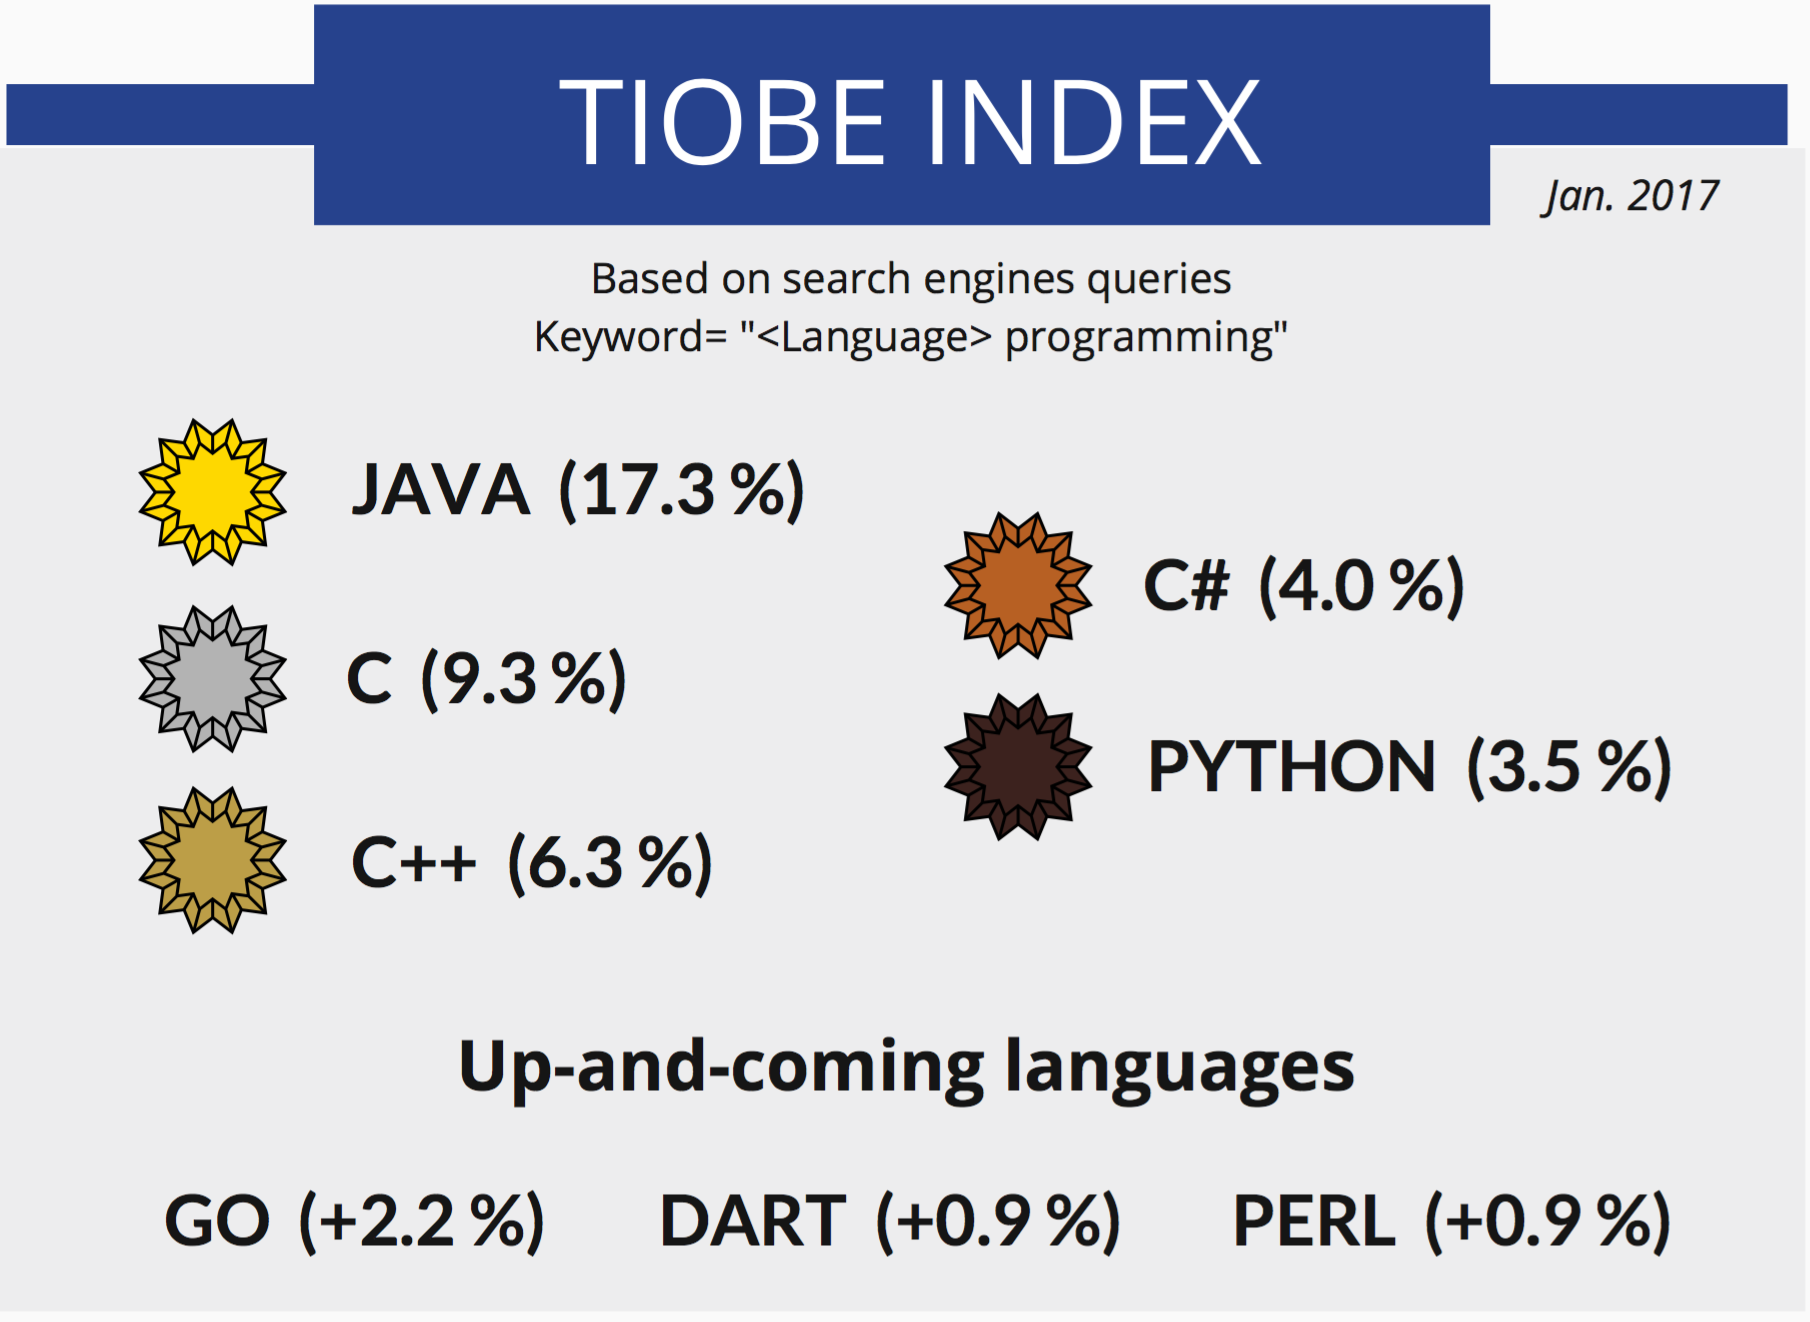
\includegraphics[scale=0.3]{\pythonroot/images/TIOBE_INDEX_2017.png}
  \caption{2017年TIOBE编程语言排行榜}
  \label{fig:TIOBE_INDEX_2017}
\end{figure}

\begin{figure}[ht]
  \centering
  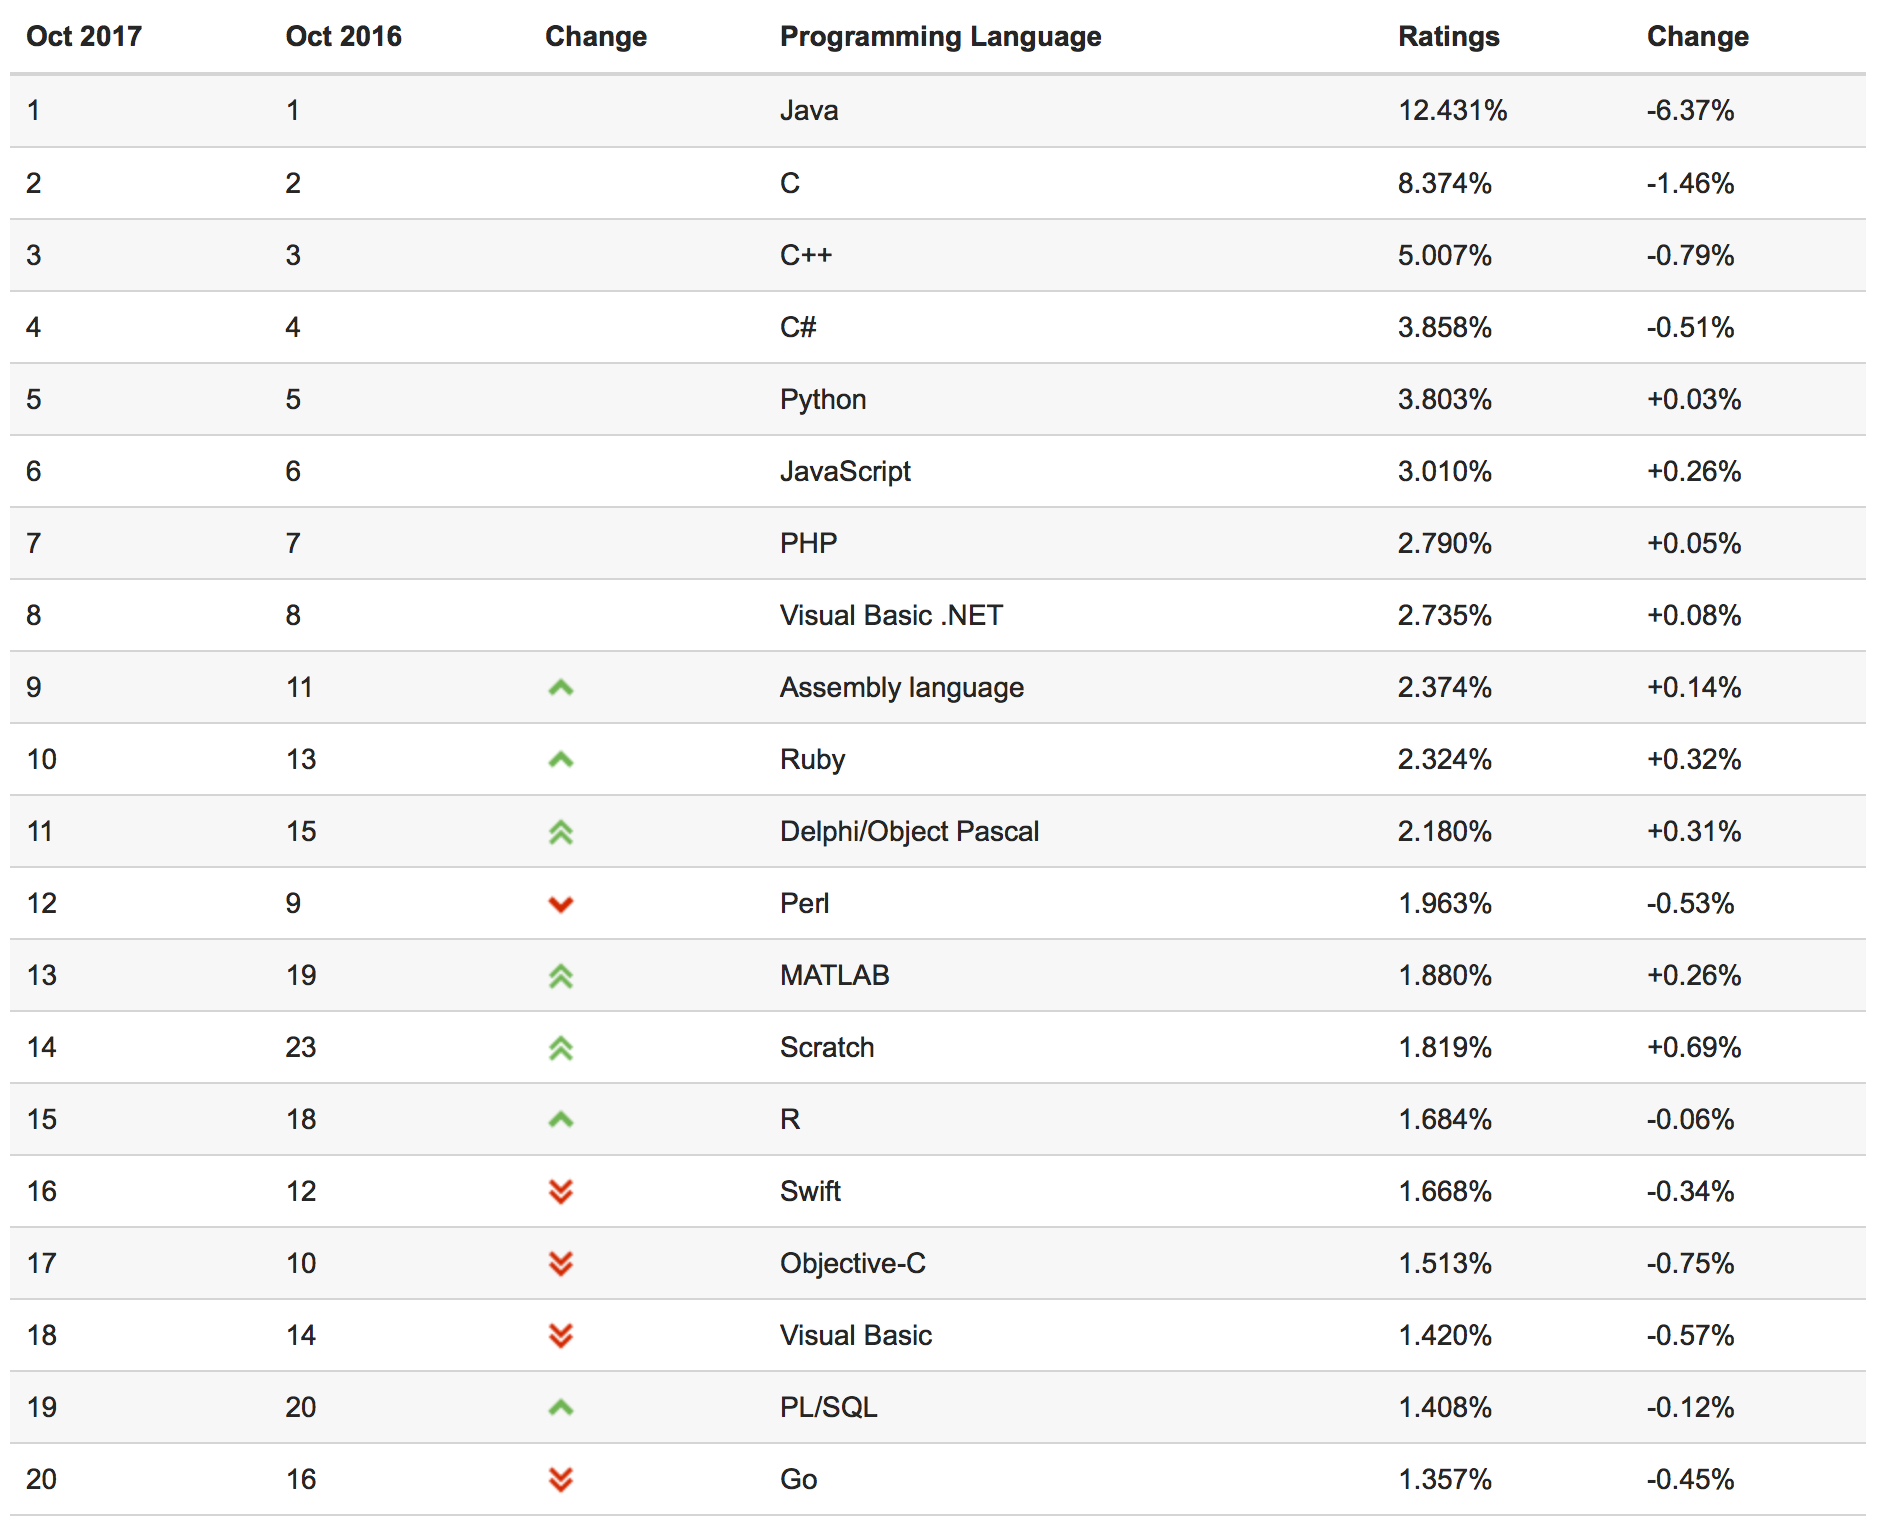
\includegraphics[scale=0.4]{\pythonroot/images/TIOBE_Index_for_January_2017.png}
  \caption{2017年1月TIOBE编程语言排行榜,来源:\href{http://www.tiobe.com/tiobe-index//}{TIOBE Index for January 2017}}
  \label{fig:TIOBE_Index_for_January_2017}
\end{figure}

\begin{figure}[ht]
  \centering
  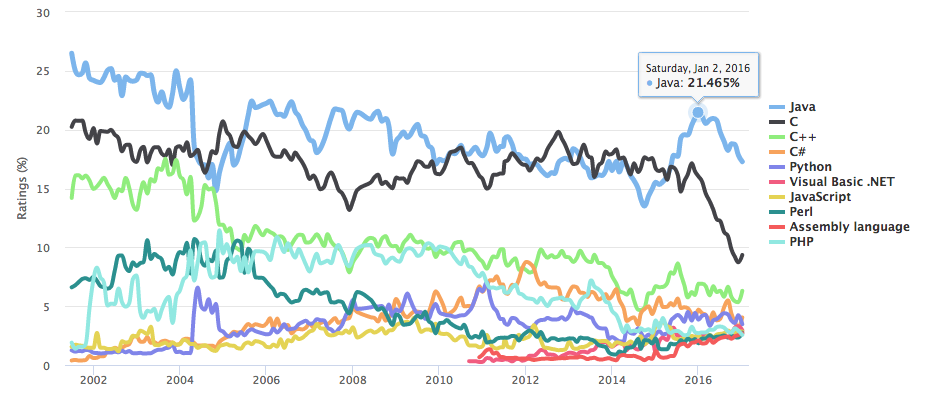
\includegraphics[scale=0.5]{\pythonroot/images/Evolution_of_the_top_10_languages_according_to_Tiobe.png}
  \caption{2017年TIOBE十大编程语言的演变,来源:\href{http://www.tiobe.com/tiobe-index//}{TIOBE Index for January 2017}}
  \label{fig:TIOBE_Top10_LANGUAGE_EVOLUTION}
\end{figure}

\begin{figure}[ht]
  \centering
  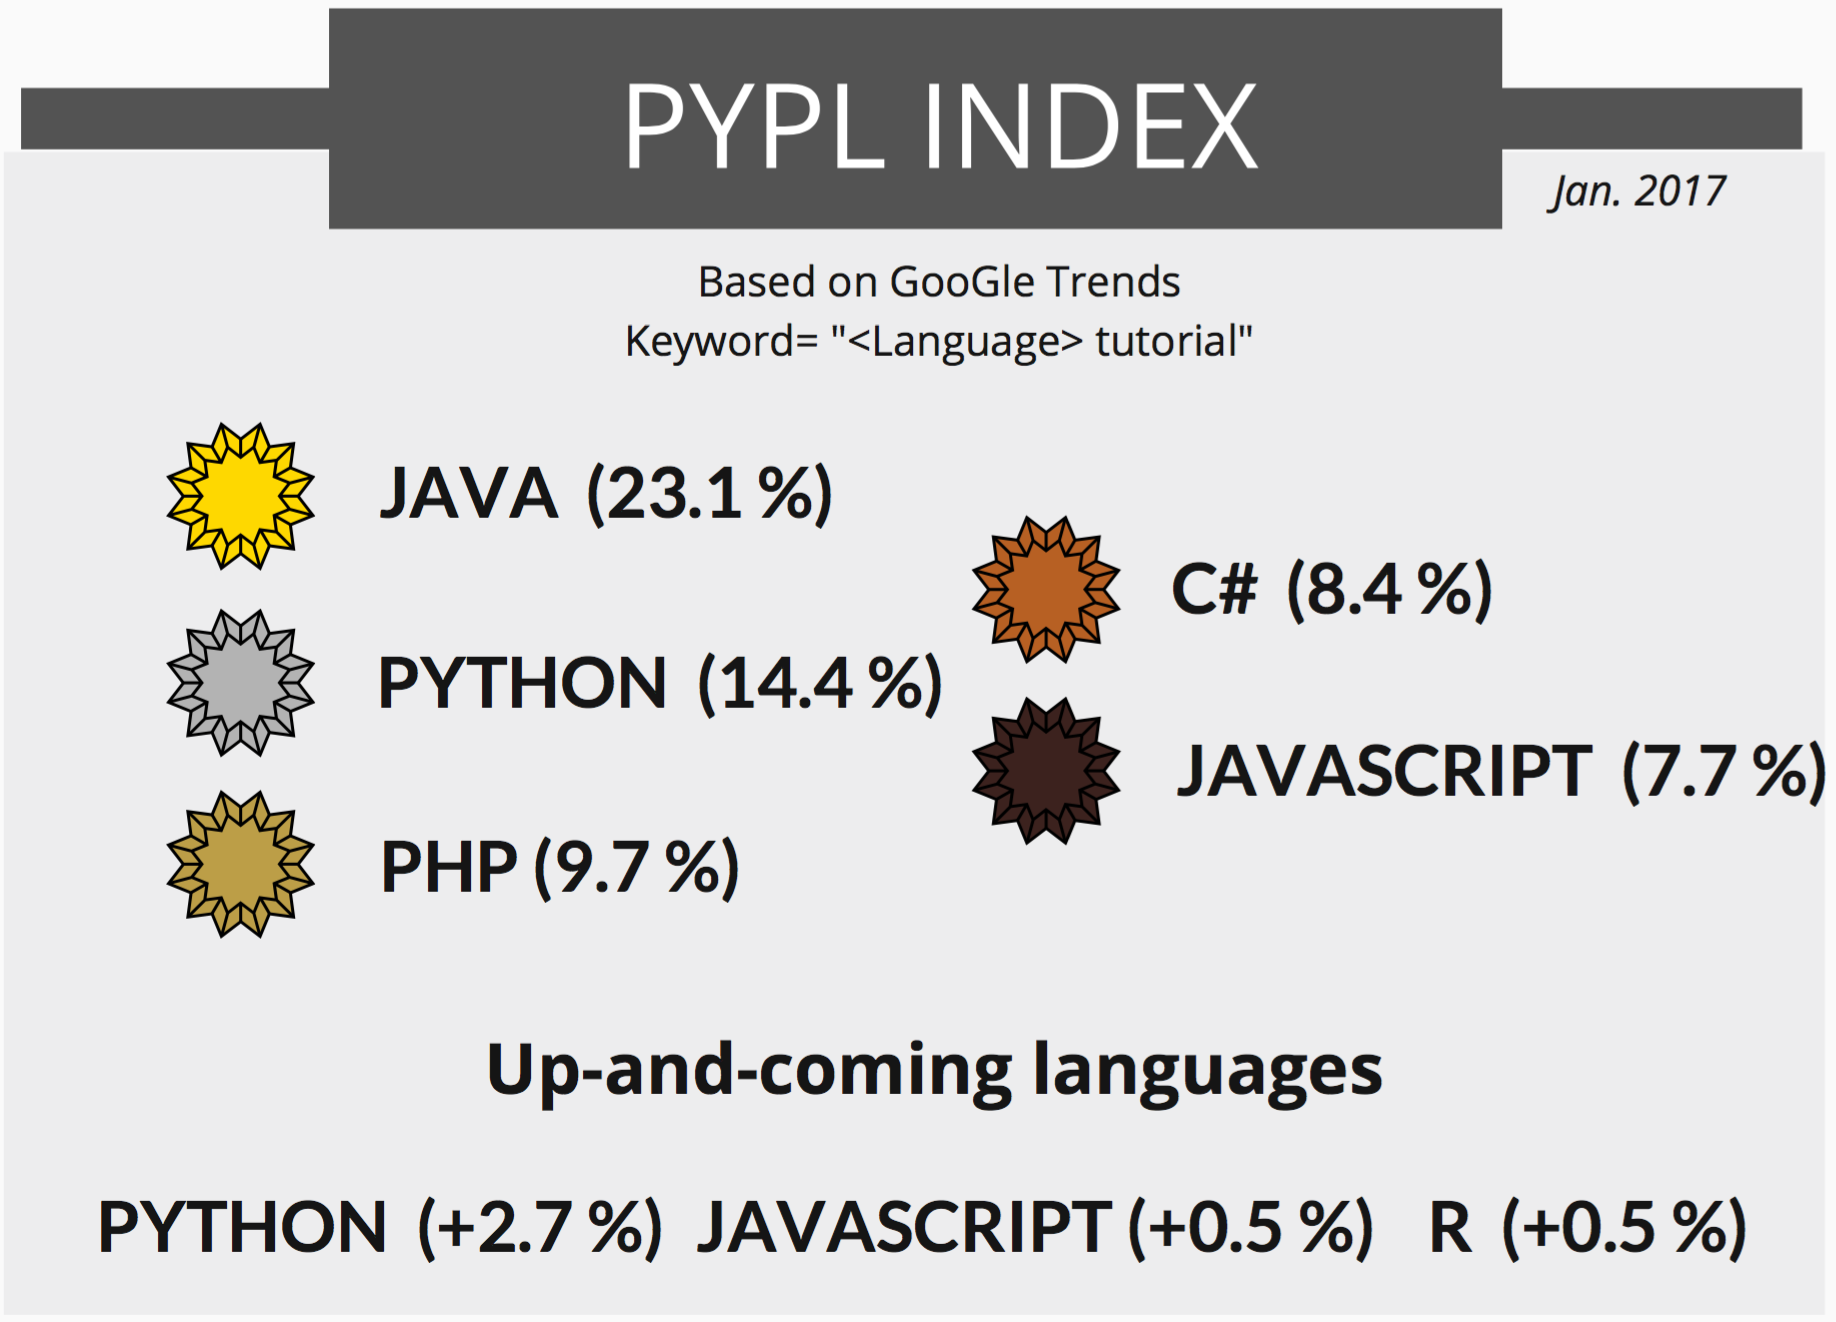
\includegraphics[scale=0.3]{\pythonroot/images/PYPL_INDEX_2017.png}
  \caption{2017年PYPL编程语言人气指数}
  \label{fig:PYPL_INDEX_2017}
\end{figure}

\begin{figure}[ht]
  \centering
  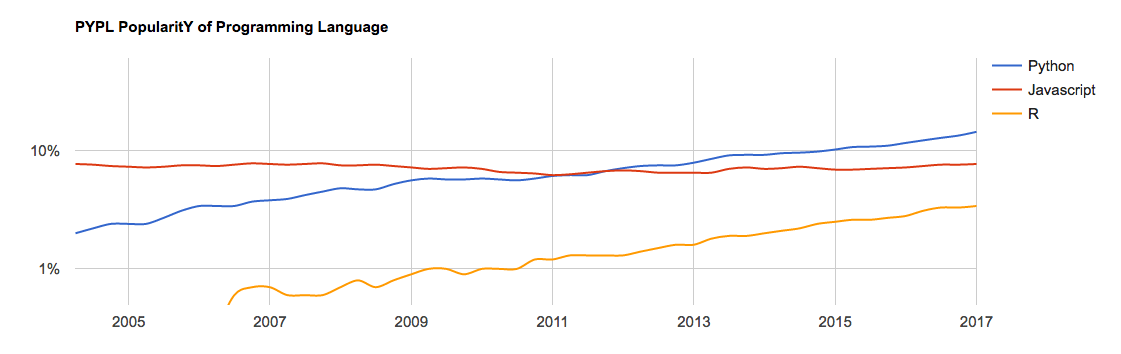
\includegraphics[scale=0.4]{\pythonroot/images/PYPL_PopularitY_of_Programming_Language.png}
  \caption{2017年PYPL编程语言人气指数,来源:\href{http://pypl.github.io/PYPL.html}{PYPL PopularitY of Programming Language Index, January 2017}}
  \label{fig:PYPL_PopularitY_of_Programming_Language}
\end{figure}


\begin{figure}[ht]
  \centering
  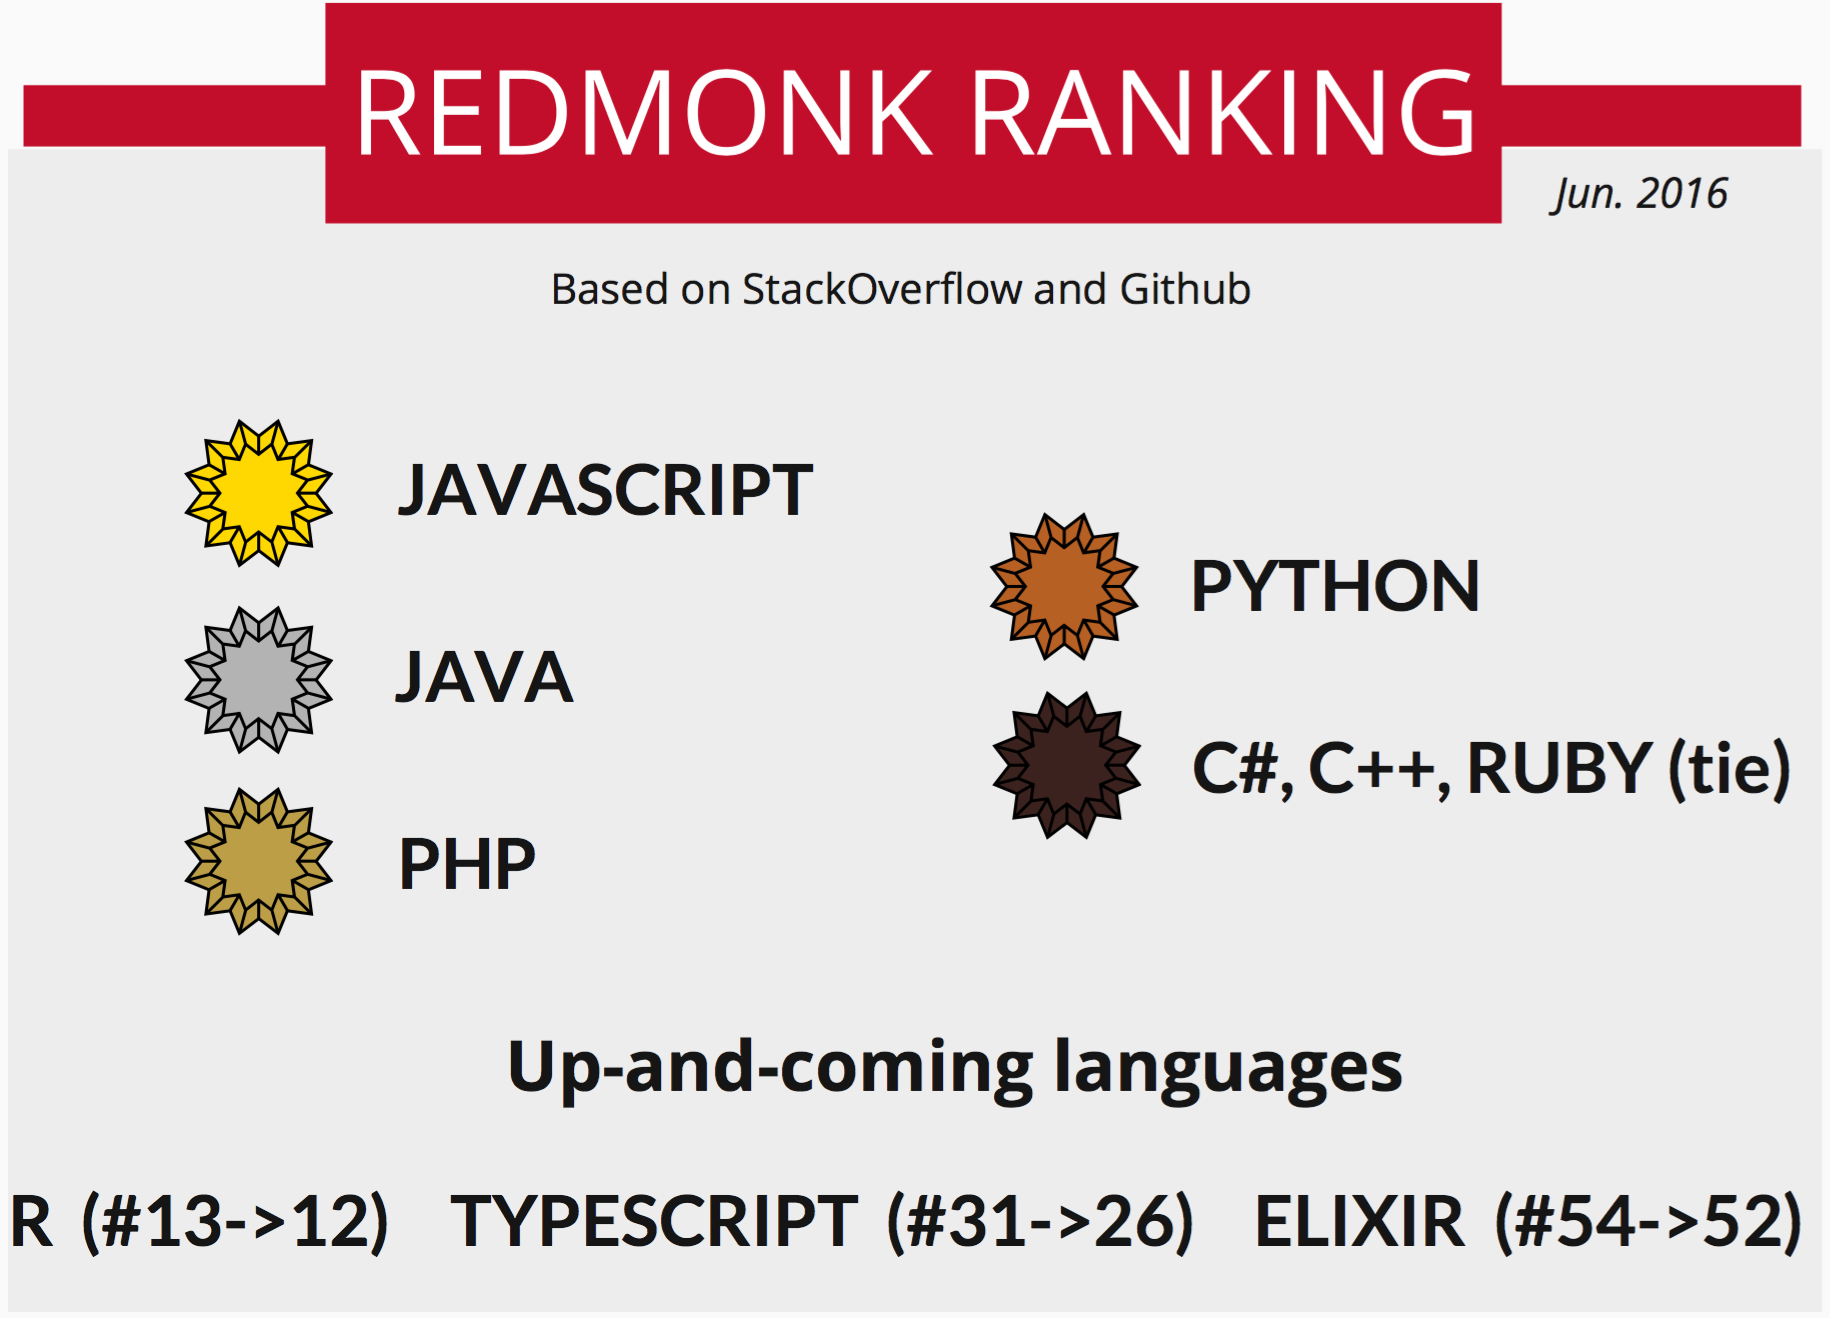
\includegraphics[scale=0.3]{\pythonroot/images/REDMONK_RANKING_2017.png}
  \caption{RedMonk编程语言排行榜}
  \label{fig:REDMONK_RANKING_2017}
\end{figure}

总的来说,这几种编程语言各有千秋。C语言是可以用来编写操作系统的贴近硬件的语言,所以,C语言适合开发那些追求运行速度、充分发挥硬件性能的程序。而Python是用来编写应用程序的高级编程语言。

当你用一种语言开始作真正的软件开发时,你除了编写代码外,还需要很多基本的已经写好的现成的东西,来帮助你加快开发进度。比如说,要编写一个电子邮件客户端,如果先从最底层开始编写网络协议相关的代码,那估计一年半载也开发不出来。高级编程语言通常都会提供一个比较完善的基础代码库,让你能直接调用,比如,针对电子邮件协议的SMTP库,针对桌面环境的GUI库,在这些已有的代码库的基础上开发,一个电子邮件客户端几天就能开发出来。

Python就为我们提供了非常完善的基础代码库,覆盖了网络、文件、GUI、数据库、文本等大量内容,被形象地称作``内置电池(batteries included)"。用Python开发,许多功能不必从零编写,直接使用现成的即可。

除了内置的库外,Python还有大量的第三方库,也就是别人开发的,供你直接使用的东西。当然,如果你开发的代码通过很好的封装,也可以作为第三方库给别人使用。

许多大型网站就是用Python开发的,例如YouTube、Instagram,还有国内的豆瓣。很多大公司,包括Google、Yahoo等,甚至NASA(美国航空航天局)都大量地使用Python。

龟叔给Python的定位是``优雅"、``明确"、``简单",所以Python程序看上去总是简单易懂,初学者学Python,不但入门容易,而且将来深入下去,可以编写那些非常非常复杂的程序。

总的来说,Python的哲学就是简单优雅,尽量写容易看明白的代码,尽量写少的代码。如果一个资深程序员向你炫耀他写的晦涩难懂、动不动就几万行的代码,你可以尽情地嘲笑他。

那Python适合开发哪些类型的应用呢?

首选是网络应用,包括网站、后台服务等等;

其次是许多日常需要的小工具,包括系统管理员需要的脚本任务等等;

另外就是把其他语言开发的程序再包装起来,方便使用。

最后说说Python的缺点。

任何编程语言都有缺点,Python也不例外。优点说过了,那Python有哪些缺点呢?

第一个缺点就是运行速度慢,和C程序相比非常慢,因为Python是解释型语言,你的代码在执行时会一行一行地翻译成CPU能理解的机器码,这个翻译过程非常耗时,所以很慢。而C程序是运行前直接编译成CPU能执行的机器码,所以非常快。

但是大量的应用程序不需要这么快的运行速度,因为用户根本感觉不出来。例如开发一个下载MP3的网络应用程序,C程序的运行时间需要0.001秒,而Python程序的运行时间需要0.1秒,慢了100倍,但由于网络更慢,需要等待1秒,你想,用户能感觉到1.001秒和1.1秒的区别吗?这就好比F1赛车和普通的出租车在北京三环路上行驶的道理一样,虽然F1赛车理论时速高达400公里,但由于三环路堵车的时速只有20公里,因此,作为乘客,你感觉的时速永远是20公里。

不要在意程序运行速度

第二个缺点就是代码不能加密。如果要发布你的Python程序,实际上就是发布源代码,这一点跟C语言不同,C语言不用发布源代码,只需要把编译后的机器码(也就是你在Windows上常见的xxx.exe文件)发布出去。要从机器码反推出C代码是不可能的,所以,凡是编译型的语言,都没有这个问题,而解释型的语言,则必须把源码发布出去。

这个缺点仅限于你要编写的软件需要卖给别人挣钱的时候。好消息是目前的互联网时代,靠卖软件授权的商业模式越来越少了,靠网站和移动应用卖服务的模式越来越多了,后一种模式不需要把源码给别人。

再说了,现在如火如荼的开源运动和互联网自由开放的精神是一致的,互联网上有无数非常优秀的像Linux一样的开源代码,我们千万不要高估自己写的代码真的有非常大的``商业价值"。那些大公司的代码不愿意开放的更重要的原因是代码写得太烂了,一旦开源,就没人敢用他们的产品了。

当然,Python还有其他若干小缺点,请自行忽略,就不一一列举了。

\subsection{安装Python}
因为Python是跨平台的,它可以运行在Windows、Mac和各种Linux/Unix系统上。在Windows上写Python程序,放到Linux上也是能够运行的。

要开始学习Python编程,首先就得把Python安装到你的电脑里。安装后,你会得到Python解释器(就是负责运行Python程序的),一个命令行交互环境,还有一个简单的集成开发环境。

目前,Python有两个版本,一个是2.x版,一个是3.x版,这两个版本是不兼容的,因为现在Python正在朝着3.x版本进化,在进化过程中,大量的针对2.x版本的代码要修改后才能运行,所以,目前有许多第三方库还暂时无法在3.x上使用。

\section{Python基础}
\subsection{第一个Python程序}
在交互式环境的提示符>>>下,直接输入代码,按回车,就可以立刻得到代码执行结果。
\begin{minted}[mathescape,
               numbersep=5pt,
               frame=lines,
               framesep=2mm]{python}
Python 2.7.12 (default, Dec  1 2016, 20:44:50) 
[GCC 4.2.1 Compatible Apple LLVM 8.0.0 (clang-800.0.42.1)] on darwin
Type "help", "copyright", "credits" or "license" for more information.
>>> print 'Hello World'
Hello World
>>> print('Hello World')
Hello World
\end{minted}

也可以将代码保存在脚本文件中,然后调用python解析器来执行程序。
\begin{minted}[mathescape,
               numbersep=5pt,
               frame=lines,
               framesep=2mm]{python}
$ cat script.py
print 'Hello World'
print('Hello World')

$ python script.py
Hello World
Hello World
\end{minted}

\subsection{Python缩进}
缩进的语句视为代码块,缩进有利有弊。好处是强迫你写出格式化的代码,但没有规定缩进是几个空格还是Tab。按照约定俗成的管理,应该始终坚持使用4个空格的缩进。

缩进的另一个好处是强迫你写出缩进较少的代码,你会倾向于把一段很长的代码拆分成若干函数,从而得到缩进较少的代码。

缩进的坏处就是“复制-粘贴”功能失效了,这是最坑爹的地方。当你重构代码时,粘贴过去的代码必须重新检查缩进是否正确。此外,IDE很难像格式化Java代码那样格式化Python代码。


\subsection{Python标识符}
在Python里,标识符由字母、数字、下划线组成,区分大小写并且不能以数字开头。以下划线开头的标识符是有特殊意义的。以单下划线开头\_foo的代表不能直接访问的类属性,需通过类提供的接口进行访问,不能用from xxx import * 而导入;以双下划线开头的 \_\_foo 代表类的私有成员;以双下划线开头和结尾的 \_\_foo\_\_ 代表 Python 里特殊方法专用的标识,如 \_\_init\_\_() 代表类的构造函数。

Python可以同一行显示多条语句,方法是用分号 ; 分开,如:
\begin{minted}[mathescape,
               numbersep=5pt,
               frame=lines,
               framesep=2mm]{python}
>>> print('hello');print('runoob');
hello
runoob
\end{minted}

\subsection{Python注释}
Python的单行注释使用\#,多行注释采用'''或者""",例如:
\begin{minted}[mathescape,
               linenos,
               numbersep=5pt,
               frame=lines,
               framesep=2mm]{python}
# coding: utf8
# 文件名:test.py

# 第一个注释
print("Hello World")  # 第二个注释
\end{minted}

\begin{minted}[mathescape,
               numbersep=5pt,
               framesep=2mm]{python}
$ python test.py
Hello World
$ 
\end{minted}


\begin{minted}[mathescape,
               %linenos,
               numbersep=5pt,
               frame=lines,
               framesep=2mm]{python}
# coding: utf8
# 文件名:test.py

'''
这是多行注释,使用单引号。
这是多行注释,使用单引号。
这是多行注释,使用单引号。
'''

"""
这是多行注释,使用双引号。
这是多行注释,使用双引号。
这是多行注释,使用双引号。
"""
\end{minted}

\subsection{Python数据类型}
\subsubsection{字符串}
\begin{minted}[mathescape,
               %linenos,
               numbersep=5pt,
               frame=lines,
               framesep=2mm]{python}

>>> s = 'Hello World'
>>> print(s)           # 输出完整字符串
Hello World
>>> print(s[0])        # 输出字符串中的第一个字符
H
>>> print(s[2:5])      # 输出字符串中第三个至第五个之间的字符串
llo
>>> print(s[2:])       # 输出从第三个字符开始的字符串
llo World
>>> print(s * 2)       # 输出字符串两次
Hello WorldHello World
>>> print(s + "TEST")  # 输出连接的字符串
Hello WorldTEST
\end{minted}

\begin{minted}[mathescape,
               %linenos,
               numbersep=5pt,
               frame=lines,
               framesep=2mm]{python}
from __future__ import division
from __future__ import print_function
...
\end{minted}



\subsubsection{列表}
\begin{minted}[mathescape,
               %linenos,
               numbersep=5pt,
               frame=lines,
               framesep=2mm]{python}

>>> lt = ['runoob', 786, 2.23, 'john', 70.2]
>>> tinylist = [123, 'john']
>>> print(lt)               # 输出完整列表
['runoob', 786, 2.23, 'john', 70.2]
>>> print(lt[0])            # 输出列表的第一个元素
runoob
>>> print(lt[1:3])          # 输出第二个至第三个的元素 
[786, 2.23]
>>> print(lt[2:])           # 输出从第三个开始至列表末尾的所有元素
[2.23, 'john', 70.2]
>>> print(tinylist * 2)     # 输出列表两次
[123, 'john', 123, 'john']
>>> print(lt + tinylist)    # 打印组合的列表
['runoob', 786, 2.23, 'john', 70.2, 123, 'john']
\end{minted}

\subsubsection{字典}
\begin{minted}[mathescape, numbersep=5pt, frame=lines, framesep=2mm]{python}
>>> d = {}
>>> d['one'] = "This is one"
>>> d[2] = "This is two"
>> tinydict = {'name': 'john','code':6734, 'dept': 'sales'}
>>> print(d['one'])          # 输出键为'one' 的值
This is one
>>> print(d[2])              # 输出键为 2 的值
This is two
>>> print(tinydict)          # 输出完整的字典
{'dept': 'sales', 'code': 6734, 'name': 'john'}
>>> print(tinydict.keys())   # 输出所有键
['dept', 'code', 'name']
>>> print(tinydict.values()) # 输出所有值
['sales', 6734, 'john']
\end{minted}

\subsubsection{循环控制语句}

\begin{minted}[mathescape, numbersep=5pt, frame=lines, framesep=2mm]{python}
if 判断条件一:
    执行语句一 ...
elif 判断条件二:
    执行语句二 ...
else:
    执行语句三 ...
\end{minted}

\begin{minted}[mathescape, numbersep=5pt, frame=lines, framesep=2mm]{python}
while 判断条件:
    执行语句……
\end{minted}

\begin{minted}[mathescape, numbersep=5pt, frame=lines, framesep=2mm]{python}
for iterating_var in sequence:
    statements(s)
\end{minted}

\subsubsection{函数定义}
你可以定义一个由自己想要功能的函数,以下是简单的规则:
\begin{itemize}
\item 函数代码块以 def 关键词开头,后接函数标识符名称和圆括号()。
\item 任何传入参数和自变量必须放在圆括号中间。圆括号之间可以用于定义参数。
\item 函数的第一行语句可以选择性地使用文档字符串—用于存放函数说明。
\item 函数内容以冒号起始,并且缩进。
\item return [表达式] 结束函数,选择性地返回一个值给调用方。不带表达式的return相当于返回 None。
\end{itemize}

\begin{minted}[mathescape, numbersep=5pt, frame=lines, framesep=2mm]{python}
def functionname(parameters):
    "函数_文档字符串"
    function_suite
    return [expression]
\end{minted}

\subsubsection{特殊函数}
Python内置了一些特殊函数,这些函数很具python特性。可以让代码更加简洁。

\begin{enumerate}
\item filter(function, sequence):
\begin{minted}[mathescape, numbersep=5pt, frame=lines, framesep=2mm]{python}
# Python 2
s = ['a', 'b', 'c', 'd']
def fun1(s):
    return True if s != 'a' else False
ret = filter(fun1, s)
print(ret)
## ['b', 'c', 'd']
\end{minted}

\begin{minted}[mathescape, numbersep=5pt, frame=lines, framesep=2mm]{python}
# Python 3
s = ['a', 'b', 'c', 'd']
def fun1(s):
    return True if s != 'a' else False
ret = filter(fun1, s)
print(ret)
# <filter object at 0x106490940>
print(list(ret))
## ['b', 'c', 'd']
\end{minted}

对sequence中的item依次执行function(item),将执行结果为True的item组成一个List/String/Tuple(取决于sequence的类型)返回。
可以看作是过滤函数。

\item map(function, sequence) 
\begin{minted}[mathescape, numbersep=5pt, frame=lines, framesep=2mm]{python}
# Python 2
s = ['a', 'b', 'c', 'd'] 
def fun2(s):
    return s + ".txt"
ret = map(fun2, s)
print(ret)
# ['a.txt', 'b.txt', 'c.txt', 'd.txt']
\end{minted}


\newpage
\begin{minted}[mathescape, numbersep=5pt, frame=lines, framesep=2mm]{python}
# Python 3
s = ['a', 'b', 'c', 'd'] 
def fun2(s):
    return s + ".txt"
ret = map(fun2, s)
print(ret)
# <map object at 0x10449ea58>
print(list(ret))
# ['a.txt', 'b.txt', 'c.txt', 'd.txt']
\end{minted}

对sequence中的item依次执行function(item),见执行结果组成一个List返回:

map也支持多个sequence,这就要求function也支持相应数量的参数输入:
\begin{minted}[mathescape, numbersep=5pt, frame=lines, framesep=2mm]{python}
def add(x, y):
    return x + y 

print map(add, range(10), range(10)) 
##[0, 2, 4, 6, 8, 10, 12, 14, 16, 18]
\end{minted}

\item reduce(function, sequence, starting\_value)
\begin{minted}[mathescape, numbersep=5pt, frame=lines, framesep=2mm]{python}
from functools import reduce # for python 3
def add1(x,y):
    return x + y
print(reduce(add1, range(1, 100)))
print(reduce(add1, range(1, 100), 20))
# 4950 (注:1+2+...+99)
# 4970 (注:1+2+...+99+20)
\end{minted}

对sequence中的item顺序迭代调用function,如果有starting\_value,还可以作为初始值调用。


\item lambda:
    \newpage
\begin{minted}[mathescape, numbersep=5pt, frame=lines, framesep=2mm]{python}
g = lambda s: s + ".fsh"
print(g("haha"))
print((lambda x: x * 2)(3))

## haha.fsh
## 6
\end{minted}

这是Python支持一种有趣的语法,它允许你快速定义单行的最小函数,类似与C语言中的宏,这些叫做lambda的函数.
\end{enumerate}


\subsection{字符串和编码}

Python的字符串

搞清楚了令人头疼的字符编码问题后,我们再来研究Python对Unicode的支持。

因为Python的诞生比Unicode标准发布的时间还要早,所以最早的Python只支持ASCII编码,普通的字符串'ABC'在Python内部都是ASCII编码的。Python提供了ord()和chr()函数,可以把字母和对应的数字相互转换:

>>> ord('A')
65
>>> chr(65)
'A'
Python在后来添加了对Unicode的支持,以Unicode表示的字符串用u'...'表示,比如:

>>> print u'中文'
中文
>>> u'中'
%u'\u4e2d'
%写u'中'和u'\u4e2d'是一样的,\u后面是十六进制的Unicode码。因此,u'A'和u'\u0041'也是一样的。

两种字符串如何相互转换?字符串'xxx'虽然是ASCII编码,但也可以看成是UTF-8编码,而u'xxx'则只能是Unicode编码。

把u'xxx'转换为UTF-8编码的'xxx'用encode('utf-8')方法:

>>> u'ABC'.encode('utf-8')
'ABC'
>>> u'中文'.encode('utf-8')
%'\xe4\xb8\xad\xe6\x96\x87'
%英文字符转换后表示的UTF-8的值和Unicode值相等(但占用的存储空间不同),而中文字符转换后1个Unicode字符将变为3个UTF-8字符,你看到的\xe4就是其中一个字节,因为它的值是228,没有对应的字母可以显示,所以以十六进制显示字节的数值。len()函数可以返回字符串的长度:

>>> len(u'ABC')
3
>>> len('ABC')
3
>>> len(u'中文')
2
%>>> len('\xe4\xb8\xad\xe6\x96\x87')
6
反过来,把UTF-8编码表示的字符串'xxx'转换为Unicode字符串u'xxx'用decode('utf-8')方法:

>>> 'abc'.decode('utf-8')
u'abc'
%>>> '\xe4\xb8\xad\xe6\x96\x87'.decode('utf-8')
%u'\u4e2d\u6587'
%>>> print '\xe4\xb8\xad\xe6\x96\x87'.decode('utf-8')
中文
由于Python源代码也是一个文本文件,所以,当你的源代码中包含中文的时候,在保存源代码时,就需要务必指定保存为UTF-8编码。当Python解释器读取源代码时,为了让它按UTF-8编码读取,我们通常在文件开头写上这两行:

%#!/usr/bin/env python
%# -*- coding: utf-8 -*-
第一行注释是为了告诉Linux/OS X系统,这是一个Python可执行程序,Windows系统会忽略这个注释;

第二行注释是为了告诉Python解释器,按照UTF-8编码读取源代码,否则,你在源代码中写的中文输出可能会有乱码。

%如果你使用Notepad++进行编辑,除了要加上# -*- coding: utf-8 -*-外,中文字符串必须是Unicode字符串:

申明了UTF-8编码并不意味着你的.py文件就是UTF-8编码的,必须并且要确保Notepad++正在使用UTF-8 without BOM编码:

set-encoding-in-notepad++

%如果.py文件本身使用UTF-8编码,并且也申明了# -*- coding: utf-8 -*-,打开命令提示符测试就可以正常显示中文:

py-chinese-test-in-cmd

格式化

最后一个常见的问题是如何输出格式化的字符串。我们经常会输出类似'亲爱的xxx你好!你xx月的话费是xx,余额是xx'之类的字符串,而xxx的内容都是根据变量变化的,所以,需要一种简便的格式化字符串的方式。

py-str-format

在Python中,采用的格式化方式和C语言是一致的,用%实现,举例如下:

%>>> 'Hello, %s' % 'world'
%'Hello, world'
%>>> 'Hi, %s, you have $%d.' % ('Michael', 1000000)
%'Hi, Michael, you have $1000000.'
你可能猜到了,%运算符就是用来格式化字符串的。在字符串内部,%s表示用字符串替换,%d表示用整数替换,有几个%?占位符,后面就跟几个变量或者值,顺序要对应好。如果只有一个%?,括号可以省略。

常见的占位符有:

%d	整数
%f	浮点数
%s	字符串
%x	十六进制整数
其中,格式化整数和浮点数还可以指定是否补0和整数与小数的位数:

>>> '%2d-%02d' % (3, 1)
' 3-01'
>>> '%.2f' % 3.1415926
'3.14'
如果你不太确定应该用什么,%s永远起作用,它会把任何数据类型转换为字符串:

>>> 'Age: %s. Gender: %s' % (25, True)
'Age: 25. Gender: True'
对于Unicode字符串,用法完全一样,但最好确保替换的字符串也是Unicode字符串:

>>> u'Hi, %s' % u'Michael'
u'Hi, Michael'
有些时候,字符串里面的%是一个普通字符怎么办?这个时候就需要转义,用%%来表示一个%:

>>> 'growth rate: %d %%' % 7
'growth rate: 7 %'
小结

由于历史遗留问题,Python 2.x版本虽然支持Unicode,但在语法上需要'xxx'和u'xxx'两种字符串表示方式。

Python当然也支持其他编码方式,比如把Unicode编码成GB2312:

>>> u'中文'.encode('gb2312')
%'\xd6\xd0\xce\xc4'
但这种方式纯属自找麻烦,如果没有特殊业务要求,请牢记仅使用Unicode和UTF-8这两种编码方式。

在Python 3.x版本中,把'xxx'和u'xxx'统一成Unicode编码,即写不写前缀u都是一样的,而以字节形式表示的字符串则必须加上b前缀:b'xxx'。

格式化字符串的时候,可以用Python的交互式命令行测试,方便快捷。


\subsection{使用list和tuple}

使用list和tuple

Reads: 450657
list

Python内置的一种数据类型是列表:list。list是一种有序的集合,可以随时添加和删除其中的元素。

比如,列出班里所有同学的名字,就可以用一个list表示:

%>>> classmates = ['Michael', 'Bob', 'Tracy']
>>> classmates
%['Michael', 'Bob', 'Tracy']
变量classmates就是一个list。用len()函数可以获得list元素的个数:

>>> len(classmates)
3
用索引来访问list中每一个位置的元素,记得索引是从0开始的:

%>>> classmates[0]
'Michael'
%>>> classmates[1]
'Bob'
%>>> classmates[2]
'Tracy'
%>>> classmates[3]
Traceback (most recent call last):
  File "<stdin>", line 1, in <module>
IndexError: list index out of range
当索引超出了范围时,Python会报一个IndexError错误,所以,要确保索引不要越界,记得最后一个元素的索引是len(classmates) - 1。

如果要取最后一个元素,除了计算索引位置外,还可以用-1做索引,直接获取最后一个元素:

>>> classmates[-1]
'Tracy'
以此类推,可以获取倒数第2个、倒数第3个:

>>> classmates[-2]
'Bob'
>>> classmates[-3]
'Michael'
>>> classmates[-4]
Traceback (most recent call last):
  File "<stdin>", line 1, in <module>
IndexError: list index out of range
当然,倒数第4个就越界了。

list是一个可变的有序表,所以,可以往list中追加元素到末尾:

>>> classmates.append('Adam')
>>> classmates
['Michael', 'Bob', 'Tracy', 'Adam']
也可以把元素插入到指定的位置,比如索引号为1的位置:

>>> classmates.insert(1, 'Jack')
>>> classmates
['Michael', 'Jack', 'Bob', 'Tracy', 'Adam']
要删除list末尾的元素,用pop()方法:

>>> classmates.pop()
'Adam'
>>> classmates
['Michael', 'Jack', 'Bob', 'Tracy']
要删除指定位置的元素,用pop(i)方法,其中i是索引位置:

>>> classmates.pop(1)
'Jack'
>>> classmates
['Michael', 'Bob', 'Tracy']
要把某个元素替换成别的元素,可以直接赋值给对应的索引位置:

>>> classmates[1] = 'Sarah'
>>> classmates
['Michael', 'Sarah', 'Tracy']
list里面的元素的数据类型也可以不同,比如:

>>> L = ['Apple', 123, True]
list元素也可以是另一个list,比如:

>>> s = ['python', 'java', ['asp', 'php'], 'scheme']
>>> len(s)
4
要注意s只有4个元素,其中s[2]又是一个list,如果拆开写就更容易理解了:

>>> p = ['asp', 'php']
>>> s = ['python', 'java', p, 'scheme']
要拿到'php'可以写p[1]或者s[2][1],因此s可以看成是一个二维数组,类似的还有三维、四维……数组,不过很少用到。

如果一个list中一个元素也没有,就是一个空的list,它的长度为0:

>>> L = []
>>> len(L)
0
tuple

另一种有序列表叫元组:tuple。tuple和list非常类似,但是tuple一旦初始化就不能修改,比如同样是列出同学的名字:

>>> classmates = ('Michael', 'Bob', 'Tracy')
现在,classmates这个tuple不能变了,它也没有append(),insert()这样的方法。其他获取元素的方法和list是一样的,你可以正常地使用classmates[0],classmates[-1],但不能赋值成另外的元素。

不可变的tuple有什么意义?因为tuple不可变,所以代码更安全。如果可能,能用tuple代替list就尽量用tuple。

tuple的陷阱:当你定义一个tuple时,在定义的时候,tuple的元素就必须被确定下来,比如:

>>> t = (1, 2)
>>> t
(1, 2)
如果要定义一个空的tuple,可以写成():

>>> t = ()
>>> t
()
但是,要定义一个只有1个元素的tuple,如果你这么定义:

>>> t = (1)
>>> t
1
定义的不是tuple,是1这个数!这是因为括号()既可以表示tuple,又可以表示数学公式中的小括号,这就产生了歧义,因此,Python规定,这种情况下,按小括号进行计算,计算结果自然是1。

所以,只有1个元素的tuple定义时必须加一个逗号,,来消除歧义:

>>> t = (1,)
>>> t
(1,)
Python在显示只有1个元素的tuple时,也会加一个逗号,,以免你误解成数学计算意义上的括号。

最后来看一个“可变的”tuple:

>>> t = ('a', 'b', ['A', 'B'])
>>> t[2][0] = 'X'
>>> t[2][1] = 'Y'
>>> t
('a', 'b', ['X', 'Y'])
这个tuple定义的时候有3个元素,分别是'a','b'和一个list。不是说tuple一旦定义后就不可变了吗?怎么后来又变了?

别急,我们先看看定义的时候tuple包含的3个元素:

tuple-0

当我们把list的元素'A'和'B'修改为'X'和'Y'后,tuple变为:

tuple-1

表面上看,tuple的元素确实变了,但其实变的不是tuple的元素,而是list的元素。tuple一开始指向的list并没有改成别的list,所以,tuple所谓的“不变”是说,tuple的每个元素,指向永远不变。即指向'a',就不能改成指向'b',指向一个list,就不能改成指向其他对象,但指向的这个list本身是可变的!

理解了“指向不变”后,要创建一个内容也不变的tuple怎么做?那就必须保证tuple的每一个元素本身也不能变。

小结

list和tuple是Python内置的有序集合,一个可变,一个不可变。根据需要来选择使用它们。




\subsection{条件判断和循环}
条件判断

计算机之所以能做很多自动化的任务,因为它可以自己做条件判断。

比如,输入用户年龄,根据年龄打印不同的内容,在Python程序中,用if语句实现:

age = 20
if age >= 18:
    print 'your age is', age
    print 'adult'
根据Python的缩进规则,如果if语句判断是True,就把缩进的两行print语句执行了,否则,什么也不做。

也可以给if添加一个else语句,意思是,如果if判断是False,不要执行if的内容,去把else执行了:

age = 3
if age >= 18:
    print 'your age is', age
    print 'adult'
else:
    print 'your age is', age
    print 'teenager'
注意不要少写了冒号:。

当然上面的判断是很粗略的,完全可以用elif做更细致的判断:

age = 3
if age >= 18:
    print 'adult'
elif age >= 6:
    print 'teenager'
else:
    print 'kid'
elif是else if的缩写,完全可以有多个elif,所以if语句的完整形式就是:

if <条件判断1>:
    <执行1>
elif <条件判断2>:
    <执行2>
elif <条件判断3>:
    <执行3>
else:
    <执行4>
if语句执行有个特点,它是从上往下判断,如果在某个判断上是True,把该判断对应的语句执行后,就忽略掉剩下的elif和else,所以,请测试并解释为什么下面的程序打印的是teenager:

age = 20
if age >= 6:
    print 'teenager'
elif age >= 18:
    print 'adult'
else:
    print 'kid'
if判断条件还可以简写,比如写:

if x:
    print 'True'
只要x是非零数值、非空字符串、非空list等,就判断为True,否则为False。

循环

Python的循环有两种,一种是for...in循环,依次把list或tuple中的每个元素迭代出来,看例子:

names = ['Michael', 'Bob', 'Tracy']
for name in names:
    print name
执行这段代码,会依次打印names的每一个元素:

Michael
Bob
Tracy
所以for x in ...循环就是把每个元素代入变量x,然后执行缩进块的语句。

再比如我们想计算1-10的整数之和,可以用一个sum变量做累加:

sum = 0
for x in [1, 2, 3, 4, 5, 6, 7, 8, 9, 10]:
    sum = sum + x
print sum
如果要计算1-100的整数之和,从1写到100有点困难,幸好Python提供一个range()函数,可以生成一个整数序列,比如range(5)生成的序列是从0开始小于5的整数:

>>> range(5)
[0, 1, 2, 3, 4]
range(101)就可以生成0-100的整数序列,计算如下:

sum = 0
for x in range(101):
    sum = sum + x
print sum
请自行运行上述代码,看看结果是不是当年高斯同学心算出的5050。

第二种循环是while循环,只要条件满足,就不断循环,条件不满足时退出循环。比如我们要计算100以内所有奇数之和,可以用while循环实现:

sum = 0
n = 99
while n > 0:
    sum = sum + n
    n = n - 2
print sum
在循环内部变量n不断自减,直到变为-1时,不再满足while条件,循环退出。

%再议raw_input

%最后看一个有问题的条件判断。很多同学会用raw_input()读取用户的输入,这样可以自己输入,程序运行得更有意思:

%birth = raw_input('birth: ')
if birth < 2000:
    print '00前'
else:
    print '00后'
输入1982,结果却显示00后,这么简单的判断Python也能搞错?

当然不是Python的问题,在Python的交互式命令行下打印birth看看:

>>> birth
'1982'
>>> '1982' < 2000
False
>>> 1982 < 2000
True
%原因找到了!原来从raw_input()读取的内容永远以字符串的形式返回,把字符串和整数比较就不会得到期待的结果,必须先用int()把字符串转换为我们想要的整型:

%birth = int(raw_input('birth: '))
再次运行,就可以得到正确地结果。但是,如果输入abc呢?又会得到一个错误信息:

Traceback (most recent call last):
  ...
ValueError: invalid literal for int() with base 10: 'abc'
原来int()发现一个字符串并不是合法的数字时就会报错,程序就退出了。

如何检查并捕获程序运行期的错误呢?后面的错误和调试会讲到。

小结

条件判断可以让计算机自己做选择,Python的if...elif...else很灵活。

python-if

循环是让计算机做重复任务的有效的方法,有些时候,如果代码写得有问题,会让程序陷入“死循环”,也就是永远循环下去。这时可以用Ctrl+C退出程序,或者强制结束Python进程。


请试写一个死循环程序。






\subsection{使用dict和set}

Reads: 373074
dict

Python内置了字典:dict的支持,dict全称dictionary,在其他语言中也称为map,使用键-值(key-value)存储,具有极快的查找速度。

举个例子,假设要根据同学的名字查找对应的成绩,如果用list实现,需要两个list:

%names = ['Michael', 'Bob', 'Tracy']
%scores = [95, 75, 85]
给定一个名字,要查找对应的成绩,就先要在names中找到对应的位置,再从scores取出对应的成绩,list越长,耗时越长。

如果用dict实现,只需要一个“名字”-“成绩”的对照表,直接根据名字查找成绩,无论这个表有多大,查找速度都不会变慢。用Python写一个dict如下:

%>>> d = {'Michael': 95, 'Bob': 75, 'Tracy': 85}
%>>> d['Michael']
95
为什么dict查找速度这么快?因为dict的实现原理和查字典是一样的。假设字典包含了1万个汉字,我们要查某一个字,一个办法是把字典从第一页往后翻,直到找到我们想要的字为止,这种方法就是在list中查找元素的方法,list越大,查找越慢。

第二种方法是先在字典的索引表里(比如部首表)查这个字对应的页码,然后直接翻到该页,找到这个字,无论找哪个字,这种查找速度都非常快,不会随着字典大小的增加而变慢。

dict就是第二种实现方式,给定一个名字,比如'Michael',dict在内部就可以直接计算出Michael对应的存放成绩的“页码”,也就是95这个数字存放的内存地址,直接取出来,所以速度非常快。

你可以猜到,这种key-value存储方式,在放进去的时候,必须根据key算出value的存放位置,这样,取的时候才能根据key直接拿到value。

把数据放入dict的方法,除了初始化时指定外,还可以通过key放入:

>>> d['Adam'] = 67
>>> d['Adam']
67
由于一个key只能对应一个value,所以,多次对一个key放入value,后面的值会把前面的值冲掉:

>>> d['Jack'] = 90
>>> d['Jack']
90
>>> d['Jack'] = 88
>>> d['Jack']
88
如果key不存在,dict就会报错:

>>> d['Thomas']
Traceback (most recent call last):
  File "<stdin>", line 1, in <module>
KeyError: 'Thomas'
要避免key不存在的错误,有两种办法,一是通过in判断key是否存在:

>>> 'Thomas' in d
False
二是通过dict提供的get方法,如果key不存在,可以返回None,或者自己指定的value:

>>> d.get('Thomas')
>>> d.get('Thomas', -1)
-1
注意:返回None的时候Python的交互式命令行不显示结果。

要删除一个key,用pop(key)方法,对应的value也会从dict中删除:

>>> d.pop('Bob')
75
>>> d
{'Michael': 95, 'Tracy': 85}
请务必注意,dict内部存放的顺序和key放入的顺序是没有关系的。

和list比较,dict有以下几个特点:

查找和插入的速度极快,不会随着key的增加而增加;
需要占用大量的内存,内存浪费多。
而list相反:

查找和插入的时间随着元素的增加而增加;
占用空间小,浪费内存很少。
所以,dict是用空间来换取时间的一种方法。

dict可以用在需要高速查找的很多地方,在Python代码中几乎无处不在,正确使用dict非常重要,需要牢记的第一条就是dict的key必须是不可变对象。

这是因为dict根据key来计算value的存储位置,如果每次计算相同的key得出的结果不同,那dict内部就完全混乱了。这个通过key计算位置的算法称为哈希算法(Hash)。

要保证hash的正确性,作为key的对象就不能变。在Python中,字符串、整数等都是不可变的,因此,可以放心地作为key。而list是可变的,就不能作为key:

>>> key = [1, 2, 3]
>>> d[key] = 'a list'
Traceback (most recent call last):
  File "<stdin>", line 1, in <module>
TypeError: unhashable type: 'list'
set

set和dict类似,也是一组key的集合,但不存储value。由于key不能重复,所以,在set中,没有重复的key。

要创建一个set,需要提供一个list作为输入集合:

>>> s = set([1, 2, 3])
>>> s
set([1, 2, 3])
注意,传入的参数[1, 2, 3]是一个list,而显示的set([1, 2, 3])只是告诉你这个set内部有1,2,3这3个元素,显示的[]不表示这是一个list。

重复元素在set中自动被过滤:

>>> s = set([1, 1, 2, 2, 3, 3])
>>> s
set([1, 2, 3])
通过add(key)方法可以添加元素到set中,可以重复添加,但不会有效果:

>>> s.add(4)
>>> s
set([1, 2, 3, 4])
>>> s.add(4)
>>> s
set([1, 2, 3, 4])
通过remove(key)方法可以删除元素:

>>> s.remove(4)
>>> s
set([1, 2, 3])
set可以看成数学意义上的无序和无重复元素的集合,因此,两个set可以做数学意义上的交集、并集等操作:

>>> s1 = set([1, 2, 3])
>>> s2 = set([2, 3, 4])
%>>> s1 & s2
set([2, 3])
>>> s1 | s2
set([1, 2, 3, 4])
set和dict的唯一区别仅在于没有存储对应的value,但是,set的原理和dict一样,所以,同样不可以放入可变对象,因为无法判断两个可变对象是否相等,也就无法保证set内部“不会有重复元素”。试试把list放入set,看看是否会报错。

再议不可变对象

上面我们讲了,str是不变对象,而list是可变对象。

对于可变对象,比如list,对list进行操作,list内部的内容是会变化的,比如:

>>> a = ['c', 'b', 'a']
>>> a.sort()
>>> a
['a', 'b', 'c']
而对于不可变对象,比如str,对str进行操作呢:

>>> a = 'abc'
>>> a.replace('a', 'A')
'Abc'
>>> a
'abc'
虽然字符串有个replace()方法,也确实变出了'Abc',但变量a最后仍是'abc',应该怎么理解呢?

我们先把代码改成下面这样:

>>> a = 'abc'
>>> b = a.replace('a', 'A')
>>> b
'Abc'
>>> a
'abc'
要始终牢记的是,a是变量,而'abc'才是字符串对象!有些时候,我们经常说,对象a的内容是'abc',但其实是指,a本身是一个变量,它指向的对象的内容才是'abc':

a-to-str

当我们调用a.replace('a', 'A')时,实际上调用方法replace是作用在字符串对象'abc'上的,而这个方法虽然名字叫replace,但却没有改变字符串'abc'的内容。相反,replace方法创建了一个新字符串'Abc'并返回,如果我们用变量b指向该新字符串,就容易理解了,变量a仍指向原有的字符串'abc',但变量b却指向新字符串'Abc'了:

a-b-to-2-strs

所以,对于不变对象来说,调用对象自身的任意方法,也不会改变该对象自身的内容。相反,这些方法会创建新的对象并返回,这样,就保证了不可变对象本身永远是不可变的。

小结

使用key-value存储结构的dict在Python中非常有用,选择不可变对象作为key很重要,最常用的key是字符串。

tuple虽然是不变对象,但试试把(1, 2, 3)和(1, [2, 3])放入dict或set中,并解释结果。


\section{Python装饰器}
If you want to take a really deep dive, you should read these \href{https://github.com/GrahamDumpleton/wrapt/tree/develop/blog}{exhaustive articles} by Graham Dumpleton. However, if you intend to get started and getting better at reading/writing python decorators, this article should suffice.

Everything is an object in python, even functions. A function can be assigned to a variable, passed to another function and can be returned from another function. Take a look at the example below:

\begin{minted}[mathescape,
               numbersep=5pt,
               frame=lines,
               framesep=2mm]{python}
def outer_function():
    print "1. This is outer function!"
    def inner_function():
        print "2. This is inner function, inside outer function!"
    print "3. This is outside inner function, inside outer function!"
    return inner_function()
func_assign = outer_function()

# output:
# 1. This is outer function!
# 3. This is outside inner function, inside outer function!
# 2. This is inner function, inside outer function!
\end{minted}

Mark in the above execution, how the statement inside the inner function is printed at the last, consequential to inner\_function being returned, at the end of outer\_function, and the execution could be seen during the assignment.

Python decorator are the function that receive a function as an argument and return another function as return value. The assumption for a decorator is that we will pass a function as argument and the signature of the inner function in the decorator must match the function to decorate.

装饰器本质上是一个Python函数,它可以让其他函数在不需要做任何代码变动的前提下增加额外功能,装饰器的返回值也是一个函数对象。它经常用于有切面需求的场景,比如:插入日志、性能测试、事务处理、缓存、权限校验等场景。装饰器是解决这类问题的绝佳设计,有了装饰器,我们就可以抽离出大量与函数功能本身无关的雷同代码并继续重用。概括的讲,装饰器的作用就是为已经存在的对象添加额外的功能。

\subsection{函数装饰器}
Let us now, write a simple function decorator for ourselves. We will write a decorator that would measure the execution time of the function passed to it.
\begin{minted}[mathescape,
               numbersep=5pt,
               frame=lines,
               framesep=2mm]{python}
import time
def timetest(input_func):
    def timed(*args, **kwargs):
        start_time = time.time()
        result = input_func(*args, **kwargs)
        end_time = time.time()
        print "Method Name - {0}, Args - {1},\nKwargs - {2}, Time - {3}".format(
                        input_func.__name__, args, kwargs, end_time - start_time)
        return result
    return timed

@timetest
def foobar(*args, **kwargs):
    time.sleep(0.3)
    print "inside foobar"
    print args, kwargs

foobar(["hello"], a=2, b=5)
# output:
# inside foobar
# (['hello'],) {'a': 2, 'b': 5}
# Method Name - foobar, Args - (['hello'],),
# Kwargs - {'a': 2, 'b': 5}, Time - 0.30296087265
\end{minted}

We passed the function foobar to decorator named timetest. Inside decorator, function foobar is referenced as variable input\_func. The result, post execution of input\_func is referred as result.

Prepending @ to the name of the decorator, and writing the same above a function calls the decorator, and passes the function to the decorator(decorates).

\subsection{方法装饰器}
Method decorators allow overriding class properties by decorating, without having to find the calling function.

Method decorators allow overriding class properties by decorating, without having to find the calling function.
\begin{minted}[mathescape,
               numbersep=5pt,
               frame=lines,
               framesep=2mm]{python}
def method_decorator(method):
    def inner(city_instance):
        if city_instance.name == "SFO":
            print "Its a cool place to live in."
        else:
            method(city_instance)
    return inner

class City(object):
    def __init__(self, name):
        self.name = name
    @method_decorator
    def print_test(self):
        print self.name

p1 = City("SFO")
p1.print_test()

# output:
# Its a cool place to live in.
\end{minted}

In the snippet shown above, we decorate the class method print\_test. The method\_decorator prints the name of the city, if the name of city instance is not SFO.

\subsection{类装饰器}
If you want to create a callable returning another callable, the function decorator approach is easier. If you want the return to be a function, function decorators should be preferred, however if you want the decorator to return a custom object that does something different to what a function does, in that case a class decorator should be used.

With a class, you can add methods and properties to the decorated callable object, or implement operations on them. You can create descriptors that act in a special way when placed in classes (e.g. classmethod, property)

\begin{minted}[mathescape,
               numbersep=5pt,
               frame=lines,
               framesep=2mm]{python}
class decoclass(object):
    def __init__(self, f):
        self.f = f

    def __call__(self, *args, **kwargs):
        # before f actions
        print 'decorator initialised'
        self.f(*args, **kwargs)
        print 'decorator terminated'
        # after f actions

@decoclass
def klass():
    print 'class'

klass()
# output:
# decorator initialised
# class
# decorator terminated
\end{minted}

\subsection{Chaining Decorators}
The chaining of decorator is similar to how multiple inheritance can be used to construct classes. We can write as many decorator as we want and include them one by one in decoration line with decoration syntax before the definition of function to be decorated.

\begin{minted}[mathescape,
               numbersep=5pt,
               frame=lines,
               framesep=2mm]{python}
def makebold(f):
    return lambda: "<b>" + f() + "</b>"
def makeitalic(f):
    return lambda: "<i>" + f() + "</i>"
@makebold
@makeitalic
def say():
    return "Hello"
print say()

# output:
# <b><i>Hello</i></b>
\end{minted}
One thing should be kept in mind that the order of decorators we set matters. When you chain decorators, the order in which they are stacked is bottom to top.

\subsection{Functools and Wraps}
When we use a decorator, we are replacing one functions with another.

\begin{minted}[mathescape,
               numbersep=5pt,
               frame=lines,
               framesep=2mm]{python}
def decorator(func):
    """decorator docstring"""
    def inner_function(*args, **kwargs):
        """inner function docstring """
        print func.__name__ + "was called"
        return func(*args, **kwargs)
    return inner_function

@decorator
def foobar(x):
    """foobar docstring"""
    return x**2

print foobar.__name__
print foobar.__doc__
# output:
# inner_function
# inner function docstring
\end{minted}

The above observation leads us to conclude that the function foobar is being replaced by inner\_function. This means that we are losing information about the function which is being passed. functools.wraps comes to our rescue. It takes the function used in the decorator and adds the functionality of copying over the function name, docstring, arguemnets etc. Lets decorate without losing information:

\begin{minted}[mathescape,
               numbersep=5pt,
               frame=lines,
               framesep=2mm]{python}
from functools import wraps
def wrapped_decorator(func):
    """wrapped decorator docstring"""
    @wraps(func)
    def inner_function(*args, **kwargs):
        """inner function docstring """
        print func.__name__ + "was called"
        return func(*args, **kwargs)
    return inner_function

@wrapped_decorator
def foobar(x):
    """foobar docstring"""
    return x**2

print foobar.__name__
print foobar.__doc__
# output:
# foobar
# foobar docstring
\end{minted}
The above implementation preserves the information about the funciton being passed to the decorator.

How would you go about caching information inside a class based decorator?

One of the ways of doing it, is listed here.
\begin{minted}[mathescape,
               numbersep=5pt,
               frame=lines,
               framesep=2mm]{python}
from functools import wraps
def decorator(arg1, arg2):
    def inner_function(function):
        @wraps(function)
        def wrapper(*args, **kwargs):
            print "Arguements passed to decorator %s and %s" % (arg1, arg2)
            function(*args, **kwargs)
        return wrapper
    return inner_function
@decorator("arg1", "arg2")
def print_args(*args):
    for arg in args:
        print arg

print print_args(1, 2, 3)
# output:
# Arguements passed to decorator arg1 and arg2
# 1
# 2
# 3
\end{minted}

\begin{minted}[mathescape,
               numbersep=5pt,
               frame=lines,
               framesep=2mm]{python}
class ClassDecorator(object):
    def __init__(self, arg1, arg2):
        print "Arguements passed to decorator %s and %s" % (arg1, arg2)
        self.arg1 = arg1
        self.arg2 = arg2

    def __call__(self, foo, *args, **kwargs):
        def inner_func(*args, **kwargs):
            print "Args passed inside decorated function .%s and %s" % (self.arg1, self.arg2)
            return foo(*args, **kwargs)
        return inner_func

@ClassDecorator("arg1", "arg2")
def print_args(*args):
    for arg in args:
        print arg

print_args(1, 2, 3)
# output:
# Arguements passed to decorator arg1 and arg2
# Args passed inside decorated function .arg1 and arg2
# 1
# 2
# 3
\end{minted}

\section{numpy}
NumPy系统是Python的一种开源的数值计算扩展。这种工具可用来存储和处理大型矩阵,比Python自身的嵌套列表结构要高效的多。

\begin{minted}[mathescape,
               numbersep=5pt,
               frame=lines,
               framesep=2mm]{python}
>>> import numpy as np
>>> np.array(3).shape
()
>>> np.array([1]).shape
(1,)
>>> np.array([1, 2, 3]).shape
(3,)
>>> np.array([[1, 2, 3], [4, 5, 6]]).shape
(2, 3)
>>> np.array([[[1, 2, 3], [4, 5, 6]], [[7, 8, 9], [10, 11, 12]]]).shape
(2, 2, 3)
\end{minted}

\begin{minted}[mathescape,
               numbersep=5pt,
               frame=lines,
               framesep=2mm]{python}
>>> import numpy as np
>>> a = np.zeros((3, 3))
>>> a
array([[ 0.,  0.,  0.],
       [ 0.,  0.,  0.],
       [ 0.,  0.,  0.]])
>>> import numpy as np
>>> a = np.ones((3, 3))
>>> a
array([[ 1.,  1.,  1.],
       [ 1.,  1.,  1.],
       [ 1.,  1.,  1.]])
>>> import numpy as np
>>> a = np.full((3, 3), 5)
>>> a
array([[5, 5, 5],
       [5, 5, 5],
       [5, 5, 5]])
\end{minted}


\begin{minted}[mathescape, numbersep=5pt, frame=lines, framesep=2mm]{python}
>>> import numpy as np
>>> a = np.array([1, 2, 3, 4, 5, 6, 7, 8, 9])
>>> a[:3]
array([1, 2, 3])
>>> a[5:]
array([6, 7, 8, 9])
>>> a[5:8]
array([6, 7, 8])
>>> a[5]
6
>>> a[-1]
9
>>> a[-2]
8
\end{minted}


\begin{minted}[mathescape, numbersep=5pt, frame=lines, framesep=2mm]{python}
>>> import numpy as np
>>> a = np.array([[1, 2, 3], [4, 5, 6], [7, 8, 9]])
>>> a[0:2, 0:2]
array([[1, 2],
       [4, 5]])
>>> a[1, 1]
5
\end{minted}


\begin{minted}[mathescape, numbersep=5pt, frame=lines, framesep=2mm]{python}
>>> import numpy as np
>>> a = np.array([[1, 2], [3, 4], [5, 6]])
>>> index = (a > 2)
>>> print(index)
[[False False]
 [ True  True]
 [ True  True]]
>>> print(a[index])
[3 4 5 6]
>>> print(a[a > 2])
[3 4 5 6]
\end{minted}


\begin{minted}[mathescape, numbersep=5pt, frame=lines, framesep=2mm]{python}
>>> import numpy as np
>>> a = np.array([1, 2, 3, 4])
>>> b = np.array([2, 3, 4, 5])
>>> c = a * b
>>> c
array([ 2,  6, 12, 20])
\end{minted}

\begin{minted}[mathescape, numbersep=5pt, frame=lines, framesep=2mm]{python}
>>> import numpy as np
>>> a = np.array([1, 2, 3, 4])
>>> b = np.array([2, 3, 4, 5])
>>> c = np.multiply(a, b)
>>> c
array([ 2,  6, 12, 20])
\end{minted}

\begin{minted}[mathescape, numbersep=5pt, frame=lines, framesep=2mm]{python}
>>> import numpy as np
>>> a = np.array([[1, 2, 3], [4, 5, 6]])
>>> b = np.array([[6, 5], [4, 3], [2, 1]])
>>> c = a.dot(b)
>>> c
array([[20, 14],
       [56, 41]])
\end{minted}

\begin{minted}[mathescape, numbersep=5pt, frame=lines, framesep=2mm]{python}
>>> import numpy as np
>>> a = np.array([[1, 2], [3, 4]])
>>> np.sum(a)
10
>>> np.sum(a, axis=1)
array([3, 7])
>>> np.sum(a, axis=0)
array([4, 6])
\end{minted}

\begin{minted}[mathescape, numbersep=5pt, frame=lines, framesep=2mm]{python}
>>> import numpy as np
>>> a = np.array([[1, 2], [3, 4]])
>>> np.max(a)
4
>>> np.max(a, axis=0)
array([3, 4])
>>> np.max(a, axis=1)
array([2, 4])
\end{minted}

\begin{minted}[mathescape, numbersep=5pt, frame=lines, framesep=2mm]{python}
>>> import numpy as np
>>> a = np.array([[1, 2], [3, 4]])
>>> np.min(a)
1
>>> np.min(a, axis=0)
array([1, 2])
>>> np.min(a, axis=1)
array([1, 3])
\end{minted}

\begin{minted}[mathescape, numbersep=5pt, frame=lines, framesep=2mm]{python}
>>> import numpy as np
>>> a = np.array([1, 2, 3, 4, 5, 6])
>>> a.reshape((2, 3))
array([[1, 2, 3],
       [4, 5, 6]])
>>> a.reshape((3, 2))
array([[1, 2],
       [3, 4],
       [5, 6]])
\end{minted}

\begin{minted}[mathescape, numbersep=5pt, frame=lines, framesep=2mm]{python}
>>> import numpy as np
>>> a = np.array([1, 2, 3, 4, 5, 6])
>>> b = a.reshape((3, 2))
>>> b
array([[1, 2],
       [3, 4],
       [5, 6]])
>>> b.flatten()
array([1, 2, 3, 4, 5, 6])
\end{minted}

\begin{minted}[mathescape, numbersep=5pt, frame=lines, framesep=2mm]{python}
>>> import numpy as np
>>> a = np.array([[1, 2], [3, 2]])
>>> a
array([[1, 2],
       [3, 2]])
>>> a.T
array([[1, 3],
       [2, 2]])
\end{minted}


\begin{minted}[mathescape, numbersep=5pt, frame=lines, framesep=2mm]{python}
from sklearn.linear_model import LogisticRegression
lr_model = LogisticRegression()

>>> from sklearn import datasets
>>> iris = datasets.load_iris()
>>> digits = datasets.load_digits()


from sklearn.metrics import SCORERS
for i in SCORERS.keys():
    print(i)

from __future__ import print_function
from sklearn import datasets
from sklearn.cross_validation import train_test_split
from sklearn.neighbors import KNeighborsClassifier




>>> from __future__ import print_function
>>> from sklearn import datasets
>>> from sklearn.cross_validation import train_test_split
>>> from sklearn.neighbors import KNeighborsClassifier
>>> 
>>> 
>>> iris = datasets.load_iris()
>>> iris_X = iris.data
>>> iris_y = iris.target
>>> 
>>> X_train, X_test, y_train, y_test = train_test_split(iris_X, iris_y, test_size=0.3)
>>> 
>>> knn = KNeighborsClassifier()
>>> knn.fit(X_train, y_train)
KNeighborsClassifier(algorithm='auto', leaf_size=30, metric='minkowski',
           metric_params=None, n_jobs=1, n_neighbors=5, p=2,
           weights='uniform')
>>> print(knn.predict(X_test))
[0 0 0 1 2 0 2 1 2 1 1 2 0 2 1 2 1 0 1 0 2 1 0 0 2 1 2 2 1 1 0 1 1 1 0 1 2
 2 1 2 0 1 0 1 0]
>>> print(y_test)
[0 0 0 1 1 0 2 1 2 2 1 2 0 2 1 2 1 0 1 0 2 1 0 0 2 1 2 2 1 1 0 1 1 1 0 1 2
 2 1 2 0 1 0 1 0]
\end{minted}

\ifx\engineeringnotes\undefined
    \bibliography{\notesroot/reference/reference.bib}
\end{document}

\fi


\ifx\engineeringnotes\undefined
    \providecommand{\notesroot}{../..}
    \providecommand{\linuxroot}{.}

    \title{Linux}
    \author{Donald Cheung\\jianzhang9102@gmail.com}
    \date{\today\footnote{文档编写开始于2018年05月09日}}

    \documentclass[a4paper,10pt]{ctexbook}
\usepackage{xeCJK}
\usepackage{fontspec}
\usepackage{minted}
\usepackage[CJKbookmarks,colorlinks,linkcolor=red]{hyperref}
\usepackage{geometry}
\usepackage{amsmath}
\usepackage[format=hang,font=small,textfont=it]{caption}
\usepackage{float}
\usepackage{subfigure}
\usepackage[nottoc]{tocbibind}
\usepackage{bm}
\usepackage[table, x11names, dvipsnames]{xcolor}
\usepackage{color}
\usepackage{array, booktabs, boldline}
\usepackage{cellspace}
\usepackage{longtable}

\setmainfont{Times New Roman}
\setsansfont{Helvetica}
\setmonofont{Courier New}
\setCJKmainfont[BoldFont={SimHei},ItalicFont={SimHei}]{SimSun}
\setCJKsansfont{SimSun}
\setCJKmonofont{SimSun}

\setcounter{secnumdepth}{4}
\setcounter{tocdepth}{4}

\geometry{left=3.0cm,right=3.0cm,top=2.5cm,bottom=2.5cm}
\bibliographystyle{plain}

%%%%%%%%%%%%%%%%%%%%%%%%%%%%%%%%% minted setting %%%%%%%%%%%%%%%%%%%%%%%%%%%%%%%%%%%
\usemintedstyle{monokai}
\definecolor{bg}{HTML}{282828} % from https://github.com/kevinsawicki/monokai
%\defaultfontfeatures{}
\newfontfamily\noligsmonofamily[NFSSFamily=noligsmonofamily]{Courier}
\setminted{fontfamily=noligsmonofamily}

\renewcommand{\theFancyVerbLine}{%
    \sffamily \textcolor{Dandelion}{\scriptsize \oldstylenums{\arabic{FancyVerbLine}}}}

\newenvironment{jcode}[3]
{%
    \VerbatimEnvironment
    \begin{listing}[h]%
    \caption{#2}%
    \label{#3}%
    \begin{minted}[xleftmargin=18pt,
                   mathescape,
                   linenos,
                   numbersep=5pt,
                   bgcolor=bg,
                   frame=lines,
                   framesep=2mm,
                   fontsize=\footnotesize]{#1}%
}
{%
    \end{minted}
    \vspace{-25pt}%
    \end{listing}%
}
\renewcommand{\listingscaption}{代码}%from minted
\renewcommand{\listoflistingscaption}{代码列表}% from minted


\newenvironment{myquote}{\begin{quote}\kaishu\zihao{-5}}{\end{quote}}
\newcommand\degree{^\circ}
\newtheorem{thm}{定理}


\begin{document}
\maketitle
\tableofcontents
\listoflistings

\else
    \providecommand{\linuxroot}{\engineeringroot/Python}
\fi

\chapter{Linux}

\section{常用工具}
\subsection{git}

\subsubsection{Syncing a fork}
Sync a fork of a repository to keep it up-to-date with the upstream repository.

Execute the following commands in order:
\begin{enumerate}
    \item git fetch upstream
    \item git checkout master
    \item git merge upstream/master
\end{enumerate}


\ifx\engineeringnotes\undefined
    \bibliography{\notesroot/reference/reference.bib}
\end{document}

\fi


\ifx\notes\undefined
    \bibliography{\notesroot/reference/reference.bib}
\end{document}

\fi


\part{项目实战}
\def\projectsnotes{}
\ifx\notes\undefined
    \providecommand{\notesroot}{..}
    \providecommand{\projectsroot}{.}

    \title{项目实战}
    \author{Donald Cheung\\jianzhang9102@gmail.com}
    \date{\today\footnote{文档编写开始于2018年05月06日}}

    \documentclass[a4paper,10pt]{ctexbook}
\usepackage{xeCJK}
\usepackage{fontspec}
\usepackage{minted}
\usepackage[CJKbookmarks,colorlinks,linkcolor=red]{hyperref}
\usepackage{geometry}
\usepackage{amsmath}
\usepackage[format=hang,font=small,textfont=it]{caption}
\usepackage{float}
\usepackage{subfigure}
\usepackage[nottoc]{tocbibind}
\usepackage{bm}
\usepackage[table, x11names, dvipsnames]{xcolor}
\usepackage{color}
\usepackage{array, booktabs, boldline}
\usepackage{cellspace}
\usepackage{longtable}

\setmainfont{Times New Roman}
\setsansfont{Helvetica}
\setmonofont{Courier New}
\setCJKmainfont[BoldFont={SimHei},ItalicFont={SimHei}]{SimSun}
\setCJKsansfont{SimSun}
\setCJKmonofont{SimSun}

\setcounter{secnumdepth}{4}
\setcounter{tocdepth}{4}

\geometry{left=3.0cm,right=3.0cm,top=2.5cm,bottom=2.5cm}
\bibliographystyle{plain}

%%%%%%%%%%%%%%%%%%%%%%%%%%%%%%%%% minted setting %%%%%%%%%%%%%%%%%%%%%%%%%%%%%%%%%%%
\usemintedstyle{monokai}
\definecolor{bg}{HTML}{282828} % from https://github.com/kevinsawicki/monokai
%\defaultfontfeatures{}
\newfontfamily\noligsmonofamily[NFSSFamily=noligsmonofamily]{Courier}
\setminted{fontfamily=noligsmonofamily}

\renewcommand{\theFancyVerbLine}{%
    \sffamily \textcolor{Dandelion}{\scriptsize \oldstylenums{\arabic{FancyVerbLine}}}}

\newenvironment{jcode}[3]
{%
    \VerbatimEnvironment
    \begin{listing}[h]%
    \caption{#2}%
    \label{#3}%
    \begin{minted}[xleftmargin=18pt,
                   mathescape,
                   linenos,
                   numbersep=5pt,
                   bgcolor=bg,
                   frame=lines,
                   framesep=2mm,
                   fontsize=\footnotesize]{#1}%
}
{%
    \end{minted}
    \vspace{-25pt}%
    \end{listing}%
}
\renewcommand{\listingscaption}{代码}%from minted
\renewcommand{\listoflistingscaption}{代码列表}% from minted


\newenvironment{myquote}{\begin{quote}\kaishu\zihao{-5}}{\end{quote}}
\newcommand\degree{^\circ}
\newtheorem{thm}{定理}


\begin{document}
\maketitle
\tableofcontents
\listoflistings

\else
    \providecommand{\projectsroot}{\notesroot/projects}
\fi

\ifx\projectsnotes\undefined
    \providecommand{\notesroot}{../..}
    \providecommand{\lmroot}{.}

    \title{语言模型}
    \author{Donald Cheung\\jianzhang9102@gmail.com}
    \date{\today\footnote{文档编写开始于2018年05月06日}}

    \documentclass[a4paper,10pt]{ctexbook}
\usepackage{xeCJK}
\usepackage{fontspec}
\usepackage{minted}
\usepackage[CJKbookmarks,colorlinks,linkcolor=red]{hyperref}
\usepackage{geometry}
\usepackage{amsmath}
\usepackage[format=hang,font=small,textfont=it]{caption}
\usepackage{float}
\usepackage{subfigure}
\usepackage[nottoc]{tocbibind}
\usepackage{bm}
\usepackage[table, x11names, dvipsnames]{xcolor}
\usepackage{color}
\usepackage{array, booktabs, boldline}
\usepackage{cellspace}
\usepackage{longtable}

\setmainfont{Times New Roman}
\setsansfont{Helvetica}
\setmonofont{Courier New}
\setCJKmainfont[BoldFont={SimHei},ItalicFont={SimHei}]{SimSun}
\setCJKsansfont{SimSun}
\setCJKmonofont{SimSun}

\setcounter{secnumdepth}{4}
\setcounter{tocdepth}{4}

\geometry{left=3.0cm,right=3.0cm,top=2.5cm,bottom=2.5cm}
\bibliographystyle{plain}

%%%%%%%%%%%%%%%%%%%%%%%%%%%%%%%%% minted setting %%%%%%%%%%%%%%%%%%%%%%%%%%%%%%%%%%%
\usemintedstyle{monokai}
\definecolor{bg}{HTML}{282828} % from https://github.com/kevinsawicki/monokai
%\defaultfontfeatures{}
\newfontfamily\noligsmonofamily[NFSSFamily=noligsmonofamily]{Courier}
\setminted{fontfamily=noligsmonofamily}

\renewcommand{\theFancyVerbLine}{%
    \sffamily \textcolor{Dandelion}{\scriptsize \oldstylenums{\arabic{FancyVerbLine}}}}

\newenvironment{jcode}[3]
{%
    \VerbatimEnvironment
    \begin{listing}[h]%
    \caption{#2}%
    \label{#3}%
    \begin{minted}[xleftmargin=18pt,
                   mathescape,
                   linenos,
                   numbersep=5pt,
                   bgcolor=bg,
                   frame=lines,
                   framesep=2mm,
                   fontsize=\footnotesize]{#1}%
}
{%
    \end{minted}
    \vspace{-25pt}%
    \end{listing}%
}
\renewcommand{\listingscaption}{代码}%from minted
\renewcommand{\listoflistingscaption}{代码列表}% from minted


\newenvironment{myquote}{\begin{quote}\kaishu\zihao{-5}}{\end{quote}}
\newcommand\degree{^\circ}
\newtheorem{thm}{定理}


\begin{document}
\maketitle
\tableofcontents
\listoflistings

\else
    \providecommand{\lmroot}{\projectsroot/language_model}
\fi

\chapter{语言模型}
Language modeling is key to many interesting problems such as speech recognition, machine translation, or image captioning.

\section{数据集介绍}

\subsection{Penn Tree Bank}
宾州树库(Penn Tree Bank)的词性标签及含义如表 \ref{table:ptb_label} 所示。

\begin{longtable}{| p{.05\linewidth} | p{.05\linewidth} | p{.35\linewidth} | p{.30\linewidth} |}
\hline
\rowcolor{SeaGreen3!30!} \textbf{编号} & \textbf{缩写} & \textbf{英文} & \textbf{中文} \\ \hline
1 & CC & Coordinating conjunction & 并列连接词 \\ \hline
2 & CD & Cardinal number & 基数 \\ \hline
3 & DT & Determiner & 限定词 \\ \hline
4 & EX & Existential there & 存在型there \\ \hline
5 & FW & Foreign word & 外文单词 \\ \hline
6 & IN & Preposition/subord, conjunction & 介词/从属,连接词 \\ \hline
7 & JJ & Adjective & 形容词 \\ \hline
8 & JJR & Adjective, comparative & 形容词,比较级 \\ \hline
9 & JJS & Adjective, superlative & 形容词,最高级 \\ \hline
10 & LS & List item marker & 列表项标记 \\ \hline
11 & MD & Modal & 情态动词 \\ \hline
12 & NN & Noun,singular or mass & 名词,可数或不可数 \\ \hline
13 & NNS & Noun, plural & 名词,复数 \\ \hline
14 & NNP & Proper noun, singular & 专有名词,单数 \\ \hline
15 & NNPS & Proper noun, plural & 专有名词,复数 \\ \hline
16 & PDT & Predeterminer & 前位限定词 \\ \hline
17 & POS & Possessive ending & 所有格结束词 \\ \hline
18 & PRP & Personal pronoun & 人称代名词 \\ \hline
19 & PP\$ & Possessive pronoun & 物主代词,所有格代名词 \\ \hline
20 & RB & Adverb & 副词 \\ \hline
21 & RBR & Adverb, comparative & 副词,比较级 \\ \hline
22 & RBS & Adverb, superlative & 副词,最高级 \\ \hline
23 & RP & Particle & 小品词 \\ \hline
24 & SYM & Symbol(mathematical or scientific) & 符号(数学或科学) \\ \hline
25 & TO & to & To \\ \hline
26 & UH & Interjection & 感叹词 \\ \hline
27 & VB & Verb, base form & 动词,基本形态 \\ \hline
28 & VBD & Verb, past tense & 动词,过去式 \\ \hline
29 & VBG & Verb, gerund/present participle & 动词,动名词/现在分词 \\ \hline
30 & VBN & Verb, past participle & 动词,过去分词 \\ \hline
31 & VBP & Verb, non-3rd ps. sing. Present & 动词,非第三人称单数现在式 \\ \hline
32 & VBZ & Verb, 3rd ps. sing. Present & 动词,第三人称单数现在式 \\ \hline
33 & WDT & wh-determiner & wh-限定词 \\ \hline
34 & WP & wh-pronoun & wh-代词 \\ \hline
35 & WP\$ & Possessive wh-pronoun & 所有格wh-代词 \\ \hline
36 & WRB & wh-adverb & wh-副词 \\ \hline
37 & \# & Pound sign & #符号 \\ \hline
38 & \$ & Dollar sign & 美元符号 \\ \hline
39 & . & Sentence-final punctuation & 句点 \\ \hline
40 & , & Comma & 逗号 \\ \hline
41 & : & Colon, semi-colon & 冒号,分号 \\ \hline
42 & ( & Left bracket character & 左括号 \\ \hline
43 & ) & Right bracket character & 右括号 \\ \hline
44 & “ & Straight double quote & 双引号 \\ \hline
45 & ‘ & Left open single quote & 左单引号 \\ \hline
46 & “ & Left open double quote & 左双引号 \\ \hline
47 & ’ & Right close single quote & 右单引号 \\ \hline
48 & ” & Right close double quote & 右双引号 \\ \hline
\caption{PTB标注结果含义}
\label{table:ptb_label}
\centering
\end{longtable}

\subsubsection{相关材料}
\begin{enumerate}
\item \href{https://pdfs.semanticscholar.org/182c/4a4074e8577c7ba5cbbc52249e41270c8d64.pdf}{THE PENN TREEBANK: AN OVERVIEW}
\item \href{https://catalog.ldc.upenn.edu/ldc99t42}{Treebank-3}
\end{enumerate}


\section{RNN语言模型}

\subsection{相关材料}
\begin{enumerate}
\item \href{https://www.tensorflow.org/tutorials/recurrent}{TensorFlow: Recurrent Neural Networks}
\end{enumerate}

\href{http://www.fit.vutbr.cz/~imikolov/rnnlm/simple-examples.tgz}{PTB dataset from Tomas Mikolov's webpage}

The dataset is already preprocessed and contains overall 10000 different words,
including the end-of-sentence marker and a special symbol (<unk>) for rare words.
In reader.py, we convert each word to a unique integer identifier,
in order to make it easy for the neural network to process the data.

The core of the model consists of an LSTM cell that processes one word at a time and
computes probabilities of the possible values for the next word in the sentence.
The memory state of the network is initialized with a vector of zeros
and gets updated after reading each word.
For computational reasons, we will process data in mini-batches of size batch\_size.
In this example, it is important to note that current\_batch\_of\_words does not correspond to a ``sentence" of words.
Every word in a batch should correspond to a time $t$.

\ifx\projectsnotes\undefined
    \bibliography{\notesroot/reference/reference.bib}
\end{document}

\fi


\ifx\projectsnotes\undefined
    \providecommand{\notesroot}{../..}
    \providecommand{\criteoroot}{.}

    \title{Display Advertising Challenge}
    \author{Donald Cheung\\jianzhang9102@gmail.com}
    \date{\today\footnote{文档编写开始于2018年5月10日}}

    \documentclass[a4paper,10pt]{ctexbook}
\usepackage{xeCJK}
\usepackage{fontspec}
\usepackage{minted}
\usepackage[CJKbookmarks,colorlinks,linkcolor=red]{hyperref}
\usepackage{geometry}
\usepackage{amsmath}
\usepackage[format=hang,font=small,textfont=it]{caption}
\usepackage{float}
\usepackage{subfigure}
\usepackage[nottoc]{tocbibind}
\usepackage{bm}
\usepackage[table, x11names, dvipsnames]{xcolor}
\usepackage{color}
\usepackage{array, booktabs, boldline}
\usepackage{cellspace}
\usepackage{longtable}

\setmainfont{Times New Roman}
\setsansfont{Helvetica}
\setmonofont{Courier New}
\setCJKmainfont[BoldFont={SimHei},ItalicFont={SimHei}]{SimSun}
\setCJKsansfont{SimSun}
\setCJKmonofont{SimSun}

\setcounter{secnumdepth}{4}
\setcounter{tocdepth}{4}

\geometry{left=3.0cm,right=3.0cm,top=2.5cm,bottom=2.5cm}
\bibliographystyle{plain}

%%%%%%%%%%%%%%%%%%%%%%%%%%%%%%%%% minted setting %%%%%%%%%%%%%%%%%%%%%%%%%%%%%%%%%%%
\usemintedstyle{monokai}
\definecolor{bg}{HTML}{282828} % from https://github.com/kevinsawicki/monokai
%\defaultfontfeatures{}
\newfontfamily\noligsmonofamily[NFSSFamily=noligsmonofamily]{Courier}
\setminted{fontfamily=noligsmonofamily}

\renewcommand{\theFancyVerbLine}{%
    \sffamily \textcolor{Dandelion}{\scriptsize \oldstylenums{\arabic{FancyVerbLine}}}}

\newenvironment{jcode}[3]
{%
    \VerbatimEnvironment
    \begin{listing}[h]%
    \caption{#2}%
    \label{#3}%
    \begin{minted}[xleftmargin=18pt,
                   mathescape,
                   linenos,
                   numbersep=5pt,
                   bgcolor=bg,
                   frame=lines,
                   framesep=2mm,
                   fontsize=\footnotesize]{#1}%
}
{%
    \end{minted}
    \vspace{-25pt}%
    \end{listing}%
}
\renewcommand{\listingscaption}{代码}%from minted
\renewcommand{\listoflistingscaption}{代码列表}% from minted


\newenvironment{myquote}{\begin{quote}\kaishu\zihao{-5}}{\end{quote}}
\newcommand\degree{^\circ}
\newtheorem{thm}{定理}


\begin{document}
\maketitle
\tableofcontents
\listoflistings

\else
    \providecommand{\criteoroot}{\projectsroot/language_model}
\fi

\chapter{Display Advertising Challenge}

\section{数据集介绍}
\href{https://www.kaggle.com/c/criteo-display-ad-challenge}{Kaggle比赛链接}

\href{http://labs.criteo.com/2014/02/download-kaggle-display-advertising-challenge-dataset/}{数据集地址}

\section{相关材料}

\begin{enumerate}
    \item \href{https://www.csie.ntu.edu.tw/~r01922136/kaggle-2014-criteo.pdf}{3 Idiots’ Approach for Display Advertising Challenge}
    \item \href{https://github.com/zero91/kaggle-2014-criteo}{kaggle-2014-criteo}
\end{enumerate}

\ifx\projectsnotes\undefined
    \bibliography{\notesroot/reference/reference.bib}
\end{document}

\fi


\ifx\projectsnotes\undefined
    \providecommand{\notesroot}{../..}
    \providecommand{\sentencepairroot}{.}

    \title{句对匹配}
    \author{Donald Cheung\\jianzhang9102@gmail.com}
    \date{\today\footnote{文档编写开始于2018年5月17日}}

    \documentclass[a4paper,10pt]{ctexbook}
\usepackage{xeCJK}
\usepackage{fontspec}
\usepackage{minted}
\usepackage[CJKbookmarks,colorlinks,linkcolor=red]{hyperref}
\usepackage{geometry}
\usepackage{amsmath}
\usepackage[format=hang,font=small,textfont=it]{caption}
\usepackage{float}
\usepackage{subfigure}
\usepackage[nottoc]{tocbibind}
\usepackage{bm}
\usepackage[table, x11names, dvipsnames]{xcolor}
\usepackage{color}
\usepackage{array, booktabs, boldline}
\usepackage{cellspace}
\usepackage{longtable}

\setmainfont{Times New Roman}
\setsansfont{Helvetica}
\setmonofont{Courier New}
\setCJKmainfont[BoldFont={SimHei},ItalicFont={SimHei}]{SimSun}
\setCJKsansfont{SimSun}
\setCJKmonofont{SimSun}

\setcounter{secnumdepth}{4}
\setcounter{tocdepth}{4}

\geometry{left=3.0cm,right=3.0cm,top=2.5cm,bottom=2.5cm}
\bibliographystyle{plain}

%%%%%%%%%%%%%%%%%%%%%%%%%%%%%%%%% minted setting %%%%%%%%%%%%%%%%%%%%%%%%%%%%%%%%%%%
\usemintedstyle{monokai}
\definecolor{bg}{HTML}{282828} % from https://github.com/kevinsawicki/monokai
%\defaultfontfeatures{}
\newfontfamily\noligsmonofamily[NFSSFamily=noligsmonofamily]{Courier}
\setminted{fontfamily=noligsmonofamily}

\renewcommand{\theFancyVerbLine}{%
    \sffamily \textcolor{Dandelion}{\scriptsize \oldstylenums{\arabic{FancyVerbLine}}}}

\newenvironment{jcode}[3]
{%
    \VerbatimEnvironment
    \begin{listing}[h]%
    \caption{#2}%
    \label{#3}%
    \begin{minted}[xleftmargin=18pt,
                   mathescape,
                   linenos,
                   numbersep=5pt,
                   bgcolor=bg,
                   frame=lines,
                   framesep=2mm,
                   fontsize=\footnotesize]{#1}%
}
{%
    \end{minted}
    \vspace{-25pt}%
    \end{listing}%
}
\renewcommand{\listingscaption}{代码}%from minted
\renewcommand{\listoflistingscaption}{代码列表}% from minted


\newenvironment{myquote}{\begin{quote}\kaishu\zihao{-5}}{\end{quote}}
\newcommand\degree{^\circ}
\newtheorem{thm}{定理}


\begin{document}
\maketitle
\tableofcontents
\listoflistings

\else
    \providecommand{\sentencepairroot}{\projectsroot/sentence_pair_classification}
\fi

\chapter{句对匹配}

\section{数据集介绍}

\subsection{Quora Question Pairs}
官方比赛链接:\href{https://www.kaggle.com/c/quora-question-pairs}{Quora Question Pairs}

数据集链接:\url{https://pan.baidu.com/s/1mij3Nza}

\subsubsection{问题详情}
\subsubsection{背景}
Quora是美国版的知乎,月活用户超过1亿,很多人会问很类似的问题。重复问题的出现,会使得信息需求者花费更多的时间去寻找答案,而答主需要对一样的问题解答很多遍。

此数据需要解决的问题就是,判断一对问题是否是重复性问题,也就是说判断两个问题是否是同一个意思。

需要注意的是,数据集中的lable是由人为标注的,也就是说并不是100\%正确的。

\begin{table}[!htb]
    \centering
    \begin{tabular}{|Sc|c|c|c|}
        \hlineB{2}
        \rowcolor{SeaGreen3!30!} \textbf{id} & \textbf{question1} & \textbf{question2} & \textbf{is\_duplicate} \\ \hlineB{1.5}
        1 & Why my answers are collapsed? & Why is my answer collapsed at once? & 0 \\ \hlineB{1.5}
        2 & How do I post a question in Quora? & How do I ask a question in Quora? & 1 \\ \hlineB{1.5}
        3 & Can I fit my booboos in a 65ml jar? & Is 1 baba worth 55 booboo (おっぱい) ? & 0 \\
        \hlineB{2}
    \end{tabular}
    \caption{quora数据集样本示例}
    \label{table:quora_data_sample}
\end{table}

需要注意的是,原始的数据文件以 $\backslash$r$\backslash$n 表示换行符。

\subsubsection{评估}
用log loss作为评估标准。

\section{Quora Question Pairs实验}

\begin{enumerate}
\item 基于词频的cosine相似度计算:[2017-03-21 21:20]
成绩:0.75402

做法:直接使用sklearn的CountVectorizer,然后获取每个问题的切词列表,统计出频次,计算两个向量的相似度。

TODO: 
\begin{itemize}
\item 基于tf-idf特征的方法
\item 两个问题的BOW向量,直接通过LR训练
\item 获取word的Embedding向量,然后加和取平均,获得问题的向量,然后(1)计算两个向量的相似度;(2)直接拼接两个向量,接入LR训练模型
\item 使用论文`Distributed Representations of Sentences and Documents`中的想法
\item 使用fastText工具
\item 使用LSTM
\item 方法参考:https://www.kaggle.com/c/quora-question-pairs/discussion/30340
\end{itemize}



\end{enumerate}

\subsection{参考资料}

\begin{enumerate}
    \item \href{https://github.com/siarez/sentence_pair_classifier}{Tensorflow implementation of Decomposable Attention Model} \\
        这份代码参考了论文 \cite{Parikh:2016aa},并采用TensorFlow实现。

\end{enumerate}


\section{相关参考文献}

\ifx\projectsnotes\undefined
    \bibliography{\notesroot/reference/reference.bib}
\end{document}

\fi


\ifx\projectsnotes\undefined
    \providecommand{\notesroot}{../..}
    \providecommand{\gamesroot}{.}

    \title{使用机器学习打游戏}
    \author{Donald Cheung\\jianzhang9102@gmail.com}
    \date{\today\footnote{文档编写开始于2018年5月27日}}

    \documentclass[a4paper,10pt]{ctexbook}
\usepackage{xeCJK}
\usepackage{fontspec}
\usepackage{minted}
\usepackage[CJKbookmarks,colorlinks,linkcolor=red]{hyperref}
\usepackage{geometry}
\usepackage{amsmath}
\usepackage[format=hang,font=small,textfont=it]{caption}
\usepackage{float}
\usepackage{subfigure}
\usepackage[nottoc]{tocbibind}
\usepackage{bm}
\usepackage[table, x11names, dvipsnames]{xcolor}
\usepackage{color}
\usepackage{array, booktabs, boldline}
\usepackage{cellspace}
\usepackage{longtable}

\setmainfont{Times New Roman}
\setsansfont{Helvetica}
\setmonofont{Courier New}
\setCJKmainfont[BoldFont={SimHei},ItalicFont={SimHei}]{SimSun}
\setCJKsansfont{SimSun}
\setCJKmonofont{SimSun}

\setcounter{secnumdepth}{4}
\setcounter{tocdepth}{4}

\geometry{left=3.0cm,right=3.0cm,top=2.5cm,bottom=2.5cm}
\bibliographystyle{plain}

%%%%%%%%%%%%%%%%%%%%%%%%%%%%%%%%% minted setting %%%%%%%%%%%%%%%%%%%%%%%%%%%%%%%%%%%
\usemintedstyle{monokai}
\definecolor{bg}{HTML}{282828} % from https://github.com/kevinsawicki/monokai
%\defaultfontfeatures{}
\newfontfamily\noligsmonofamily[NFSSFamily=noligsmonofamily]{Courier}
\setminted{fontfamily=noligsmonofamily}

\renewcommand{\theFancyVerbLine}{%
    \sffamily \textcolor{Dandelion}{\scriptsize \oldstylenums{\arabic{FancyVerbLine}}}}

\newenvironment{jcode}[3]
{%
    \VerbatimEnvironment
    \begin{listing}[h]%
    \caption{#2}%
    \label{#3}%
    \begin{minted}[xleftmargin=18pt,
                   mathescape,
                   linenos,
                   numbersep=5pt,
                   bgcolor=bg,
                   frame=lines,
                   framesep=2mm,
                   fontsize=\footnotesize]{#1}%
}
{%
    \end{minted}
    \vspace{-25pt}%
    \end{listing}%
}
\renewcommand{\listingscaption}{代码}%from minted
\renewcommand{\listoflistingscaption}{代码列表}% from minted


\newenvironment{myquote}{\begin{quote}\kaishu\zihao{-5}}{\end{quote}}
\newcommand\degree{^\circ}
\newtheorem{thm}{定理}


\begin{document}
\maketitle
\tableofcontents
\listoflistings

\else
    \providecommand{\gamesroot}{\projectsroot/games}
\fi

\chapter{使用机器学习打游戏}

\section{贪吃蛇}


\section{Flappy Bird}

\subsection{相关材料}
\begin{enumerate}
    \item \href{https://github.com/yenchenlin/DeepLearningFlappyBird}{Flappy Bird hack using Deep Reinforcement Learning (Deep Q-learning)}
\end{enumerate}


\ifx\projectsnotes\undefined
    \bibliography{\notesroot/reference/reference.bib}
\end{document}

\fi


\chapter{依存分析}
相关资料:
\begin{enumerate}
    \item \href{http://www.hankcs.com/nlp/corpus/chinese-treebank.html}{汉语树库}
\end{enumerate}

\ifx\notes\undefined
    \bibliography{\notesroot/reference/reference.bib}
\end{document}

\fi


\part{论文笔记}
\def\papersnotes{}
\ifx\notes\undefined
    \providecommand{\notesroot}{..}
    \providecommand{\papersroot}{.}

    \title{论文笔记}
    \author{Donald Cheung\\jianzhang9102@gmail.com}
    \date{\today\footnote{文档编写开始于2018年05月17日}}

    \documentclass[a4paper,10pt]{ctexbook}
\usepackage{xeCJK}
\usepackage{fontspec}
\usepackage{minted}
\usepackage[CJKbookmarks,colorlinks,linkcolor=red]{hyperref}
\usepackage{geometry}
\usepackage{amsmath}
\usepackage[format=hang,font=small,textfont=it]{caption}
\usepackage{float}
\usepackage{subfigure}
\usepackage[nottoc]{tocbibind}
\usepackage{bm}
\usepackage[table, x11names, dvipsnames]{xcolor}
\usepackage{color}
\usepackage{array, booktabs, boldline}
\usepackage{cellspace}
\usepackage{longtable}

\setmainfont{Times New Roman}
\setsansfont{Helvetica}
\setmonofont{Courier New}
\setCJKmainfont[BoldFont={SimHei},ItalicFont={SimHei}]{SimSun}
\setCJKsansfont{SimSun}
\setCJKmonofont{SimSun}

\setcounter{secnumdepth}{4}
\setcounter{tocdepth}{4}

\geometry{left=3.0cm,right=3.0cm,top=2.5cm,bottom=2.5cm}
\bibliographystyle{plain}

%%%%%%%%%%%%%%%%%%%%%%%%%%%%%%%%% minted setting %%%%%%%%%%%%%%%%%%%%%%%%%%%%%%%%%%%
\usemintedstyle{monokai}
\definecolor{bg}{HTML}{282828} % from https://github.com/kevinsawicki/monokai
%\defaultfontfeatures{}
\newfontfamily\noligsmonofamily[NFSSFamily=noligsmonofamily]{Courier}
\setminted{fontfamily=noligsmonofamily}

\renewcommand{\theFancyVerbLine}{%
    \sffamily \textcolor{Dandelion}{\scriptsize \oldstylenums{\arabic{FancyVerbLine}}}}

\newenvironment{jcode}[3]
{%
    \VerbatimEnvironment
    \begin{listing}[h]%
    \caption{#2}%
    \label{#3}%
    \begin{minted}[xleftmargin=18pt,
                   mathescape,
                   linenos,
                   numbersep=5pt,
                   bgcolor=bg,
                   frame=lines,
                   framesep=2mm,
                   fontsize=\footnotesize]{#1}%
}
{%
    \end{minted}
    \vspace{-25pt}%
    \end{listing}%
}
\renewcommand{\listingscaption}{代码}%from minted
\renewcommand{\listoflistingscaption}{代码列表}% from minted


\newenvironment{myquote}{\begin{quote}\kaishu\zihao{-5}}{\end{quote}}
\newcommand\degree{^\circ}
\newtheorem{thm}{定理}


\begin{document}
\maketitle
\tableofcontents
\listoflistings

\else
    \providecommand{\papersroot}{\notesroot/papers}
\fi

\ifx\mlbook\undefined
    \documentclass[10pt,a4paper]{ctexbook}
    \providecommand{\pathroot}{../..}

    \usepackage[CJKbookmarks,colorlinks,linkcolor=red]{hyperref}
    \usepackage{geometry}
    \usepackage{amsmath}

    \geometry{left=3.0cm,right=3.0cm,top=2.5cm,bottom=2.5cm}
    \setmainfont{SimSun}
    \XeTeXlinebreaklocale "zh"
    \XeTeXlinebreakskip = 0pt plus 1pt minus 0.1pt

    \begin{document}
    \setlength{\baselineskip}{20pt}
    \title{自然语言处理}
    \author{Donald Cheung\\jianzhang9102@gmail.com}
    \date{Oct 27, 2017}
    \maketitle
    \tableofcontents
\fi

\chapter{自然语言处理}

\href{https://cs224d.stanford.edu}{CS224d: Deep Learning for Natural Language Processing}


\section{Word Embedding}

\section{语言模型}
\begin{itemize}
\item \href{http://www.jmlr.org/papers/volume3/bengio03a/bengio03a.pdf}{A Neural Probabilistic Language Model}
\item \href{https://arxiv.org/pdf/1708.02657.pdf}{Which Encoding is the Best for Text Classification in Chinese, English, Japanese and Korean?}
\end{itemize}

\subsubsection{相关文献}
\section{文本分类}
\section{机器翻译}
\section{序列标注}

\section{学习资料}
Course notes for CS224N Winter17: \url{https://github.com/stanfordnlp/cs224n-winter17-notes}



\ifx\mlbook\undefined
    \end{document}
\fi


\ifx\mlnotes\undefined
    \providecommand{\notesroot}{../..}
    \providecommand{\rlroot}{.}

    \title{强化学习}
    \author{Donald Cheung\\jianzhang9102@gmail.com}
    \date{\today\footnote{文档编写开始于2017年11月11日}}

    \documentclass[a4paper,10pt]{ctexbook}
\usepackage{xeCJK}
\usepackage{fontspec}
\usepackage{minted}
\usepackage[CJKbookmarks,colorlinks,linkcolor=red]{hyperref}
\usepackage{geometry}
\usepackage{amsmath}
\usepackage[format=hang,font=small,textfont=it]{caption}
\usepackage{float}
\usepackage{subfigure}
\usepackage[nottoc]{tocbibind}
\usepackage{bm}
\usepackage[table, x11names, dvipsnames]{xcolor}
\usepackage{color}
\usepackage{array, booktabs, boldline}
\usepackage{cellspace}
\usepackage{longtable}

\setmainfont{Times New Roman}
\setsansfont{Helvetica}
\setmonofont{Courier New}
\setCJKmainfont[BoldFont={SimHei},ItalicFont={SimHei}]{SimSun}
\setCJKsansfont{SimSun}
\setCJKmonofont{SimSun}

\setcounter{secnumdepth}{4}
\setcounter{tocdepth}{4}

\geometry{left=3.0cm,right=3.0cm,top=2.5cm,bottom=2.5cm}
\bibliographystyle{plain}

%%%%%%%%%%%%%%%%%%%%%%%%%%%%%%%%% minted setting %%%%%%%%%%%%%%%%%%%%%%%%%%%%%%%%%%%
\usemintedstyle{monokai}
\definecolor{bg}{HTML}{282828} % from https://github.com/kevinsawicki/monokai
%\defaultfontfeatures{}
\newfontfamily\noligsmonofamily[NFSSFamily=noligsmonofamily]{Courier}
\setminted{fontfamily=noligsmonofamily}

\renewcommand{\theFancyVerbLine}{%
    \sffamily \textcolor{Dandelion}{\scriptsize \oldstylenums{\arabic{FancyVerbLine}}}}

\newenvironment{jcode}[3]
{%
    \VerbatimEnvironment
    \begin{listing}[h]%
    \caption{#2}%
    \label{#3}%
    \begin{minted}[xleftmargin=18pt,
                   mathescape,
                   linenos,
                   numbersep=5pt,
                   bgcolor=bg,
                   frame=lines,
                   framesep=2mm,
                   fontsize=\footnotesize]{#1}%
}
{%
    \end{minted}
    \vspace{-25pt}%
    \end{listing}%
}
\renewcommand{\listingscaption}{代码}%from minted
\renewcommand{\listoflistingscaption}{代码列表}% from minted


\newenvironment{myquote}{\begin{quote}\kaishu\zihao{-5}}{\end{quote}}
\newcommand\degree{^\circ}
\newtheorem{thm}{定理}


\begin{document}
\maketitle
\tableofcontents
\listoflistings

\else
    \providecommand{\rlroot}{\mlroot/rl}
\fi

\chapter{强化学习}

on-policy vs off-policy

\section{SARAS}

\section{Q-Learning}

强化学习推荐阅读材料:
\begin{enumerate}
    \item \href{https://ai.intel.com/demystifying-deep-reinforcement-learning/}{Demystifying Deep Reinforcement Learning (Part I)}
    \item \href{https://ai.intel.com/deep-reinforcement-learning-with-neon/}{Guest Post (Part II): Deep Reinforcement Learning with Neon (Part II)}
    \item \href{http://simplecore-dev.intel.com/nervana/wp-content/uploads/sites/55/2015/12/ProofQlearning.pdf}{Convergence of Q-learning: a simple proof}
    \item \url{https://github.com/yenchenlin/DeepLearningFlappyBird}
\end{enumerate}

\section{待整理材料}

\href{https://mp.weixin.qq.com/s?__biz=MzA5MDE2MjQ0OQ==&mid=2652786766&idx=1&sn=bf6f3189e4a16b9f71f985392c9dc70b&chksm=8be52430bc92ad2644838a9728d808d000286fb9ca7ced056392f1210300286f63bd991bde84#rd}{要不我也说说 AlphaGo?}

\href{http://karpathy.github.io/2016/05/31/rl/}{Deep Reinforcement Learning: Pong from Pixels}


\section{蒙特卡罗树搜索}
\href{https://www.zhihu.com/question/39916945}{蒙特卡洛树是什么算法?}


蒙特卡罗树搜索(Monte Carlo Tree Search)并不是一种"模拟人"的算法。
而是通过随机的对游戏进行推演来逐渐建立一棵不对称的搜索树的过程。
可以看成是某种意义上的强化学习,当然这一点学界还有一些争议。

蒙特卡罗树搜索大概可以被分成四步:
选择(Selection),拓展(Expansion),模拟(Simulation),反向传播(Backpropagation)。

在开始阶段,搜索树只有一个节点,也就是我们需要决策的局面。

搜索树中的每一个节点包含了三个基本信息:代表的局面,被访问的次数,累计评分。

\begin{enumerate}
\item 选择(Selection)
在选择阶段,需要从根节点,也就是要做决策的局面R出发向下选择出一个最急迫需要被拓展的节点N,局面R是是每一次迭代中第一个被检查的节点;
对于被检查的局面而言,他可能有三种可能:
    \begin{enumerate}
    \item 该节点所有可行动作都已经被拓展过
    \item 该节点有可行动作还未被拓展过
    \item 这个节点游戏已经结束了(例如已经连成五子的五子棋局面)
    \end{enumerate}

对于这三种可能:
    \begin{enumerate}
    \item 如果所有可行动作都已经被拓展过了,那么我们将使用UCB公式计算该节点所有子节点的UCB值,并找到值最大的一个子节点继续检查。反复向下迭代。
    \item 如果被检查的局面依然存在没有被拓展的子节点(例如说某节点有20个可行动作,但是在搜索树中才创建了19个子节点),那么我们认为这个节点就是本次迭代的的目标节点N,并找出N还未被拓展的动作A。执行步骤[2]
    \item 如果被检查到的节点是一个游戏已经结束的节点。那么从该节点直接执行步骤[4]。
    \end{enumerate}
每一个被检查的节点的被访问次数在这个阶段都会自增。在反复的迭代之后,我们将在搜索树的底端找到一个节点,来继续后面的步骤。

\item 拓展(Expansion)
在选择阶段结束时候,我们查找到了一个最迫切被拓展的节点N,以及他一个尚未拓展的动作A。在搜索树中创建一个新的节点Nn作为N的一个新子节点。Nn的局面就是节点N在执行了动作A之后的局面。

\item 模拟(Simulation)为了让Nn得到一个初始的评分。我们从Nn开始,让游戏随机进行,直到得到一个游戏结局,这个结局将作为Nn的初始评分。一般使用胜利/失败来作为评分,只有1或者0。

\item 反向传播(Backpropagation)
在Nn的模拟结束之后,它的父节点N以及从根节点到N的路径上的所有节点都会根据本次模拟的结果来添加自己的累计评分。如果在[1]的选择中直接发现了一个游戏结局的话,根据该结局来更新评分。每一次迭代都会拓展搜索树,随着迭代次数的增加,搜索树的规模也不断增加。当到了一定的迭代次数或者时间之后结束,选择根节点下最好的子节点作为本次决策的结果。一次迭代的图例
\begin{figure}[ht]
    \centering
    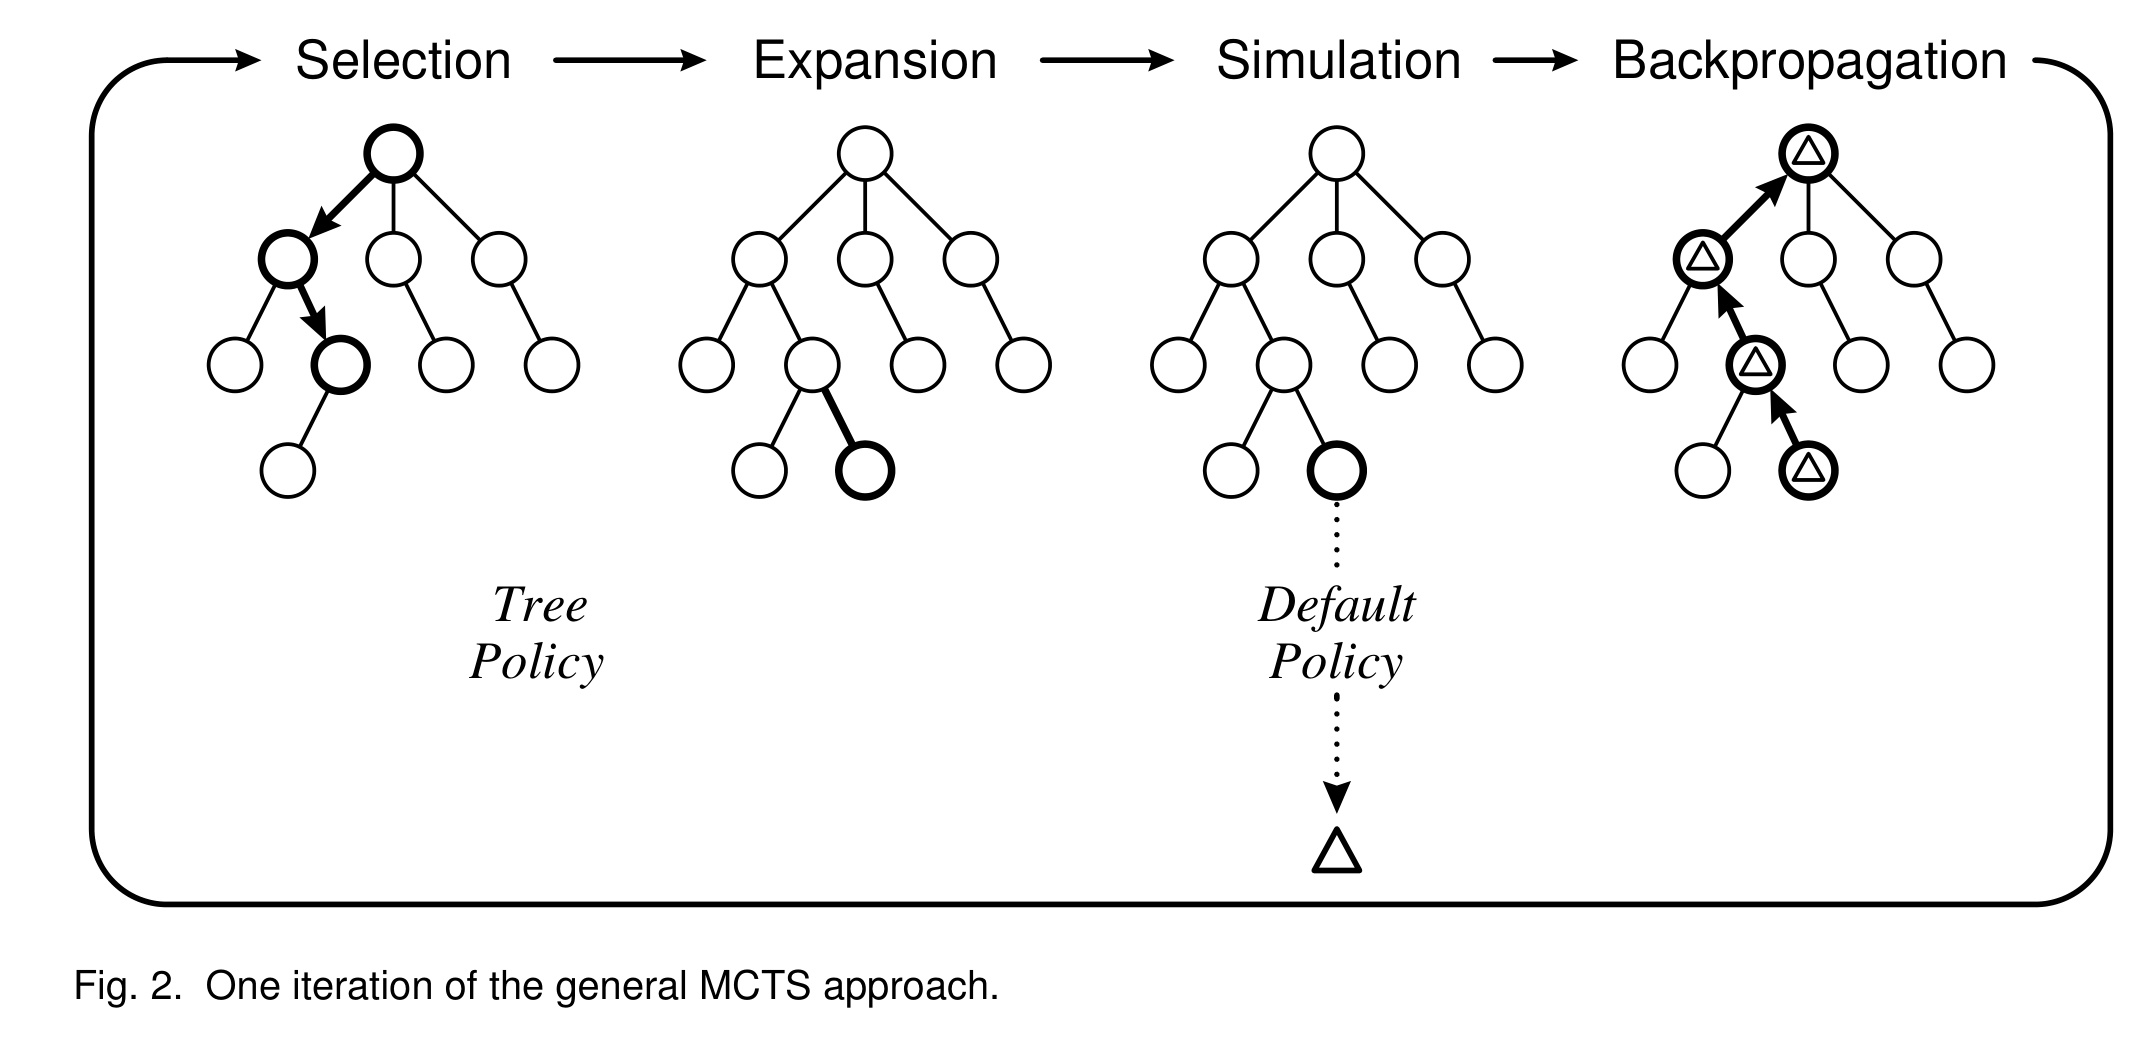
\includegraphics[height=7cm]{\rlroot/images/mcts_approach.jpg}
    \label{fig:mcts_approach}
\end{figure}

\end{enumerate}

上面描述的是UCT (UCB for Tree)算法,可以说是最经典的蒙特卡罗树搜索算法了。
但随着算法的发展,MCTS已经有了非常大的改变。
例如很多围棋AI都已经不再使用纯粹的UCB公式而改用效果更好的UCB1-Tuned了,而搜索方法上也有了非常多的改动了。

Reference:
\begin{itemize}
\item Browne C B, Powley E, Whitehouse D, et al. A Survey of Monte Carlo Tree Search Methods[J]. IEEE Transactions on Computational Intelligence \& Ai in Games, 2012, 4:1(1):1-43.
\item P. Auer, N. Cesa-Bianchi, and P. Fischer, “Finite-time Analysis  of the Multiarmed Bandit Problem,” Mach. Learn., vol. 47, no. 2,  pp. 235-256, 2002.
\end{itemize}

\section{GO}

\url{https://github.com/ardanlabs/gotraining}

\href{https://www.tastehit.com/blog/google-deepmind-alphago-how-it-works/}{Google DeepMind's AlphaGo: How it works}

\href{http://gopherdata.io/post/build_ml_powered_game_ai_tensorflow/}{Building an ML-Powered Game AI using TensorFlow in Go}

\href{https://github.com/TheDuck314/go-NN}{Go-playing neural network in Python using TensorFlow}

\begin{itemize}
\item \href{https://arxiv.org/pdf/1704.03732.pdf}{Learning from Demonstrations for Real World Reinforcement Learning}
\item \href{https://arxiv.org/abs/1312.5602}{Playing Atari with Deep Reinforcement Learning}
\item \href{https://www.intelnervana.com/demystifying-deep-reinforcement-learning/}{Guest Post (Part I): Demystifying Deep Reinforcement Learning}
\item \href{https://storage.googleapis.com/deepmind-media/dqn/DQNNaturePaper.pdf}{Human-level control through deep reinforcement learning}
\item \href{http://simplecore-dev.intel.com/nervana/wp-content/uploads/sites/55/2015/12/ProofQlearning.pdf}{Convergence of Q-learning: a simple proof}
\end{itemize}

$<s, a, r, s'>$

\subsection{贝尔曼方程(Bellman Equation)}
\href{https://zhuanlan.zhihu.com/p/21340755?refer=intelligentunit}{DQN 从入门到放弃3 价值函数与Bellman方程}

\subsection{bandit老虎机}
多臂老虎机

\ifx\mlnotes\undefined
    \bibliography{\notesroot/reference/reference.bib}
\end{document}

\fi


\chapter{图像处理}

\chapter{语音识别}

\ifx\notes\undefined
    \bibliography{\notesroot/reference/reference.bib}
\end{document}

\fi


\part{算法与数据结构}

\bibliography{\notesroot/reference/reference.bib}
\end{document}

